\documentclass[a4paper,10pt]{article}\usepackage[]{graphicx}\usepackage[]{color}
%% maxwidth is the original width if it is less than linewidth
%% otherwise use linewidth (to make sure the graphics do not exceed the margin)
\makeatletter
\def\maxwidth{ %
  \ifdim\Gin@nat@width>\linewidth
    \linewidth
  \else
    \Gin@nat@width
  \fi
}
\makeatother

\definecolor{fgcolor}{rgb}{0.345, 0.345, 0.345}
\newcommand{\hlnum}[1]{\textcolor[rgb]{0.686,0.059,0.569}{#1}}%
\newcommand{\hlstr}[1]{\textcolor[rgb]{0.192,0.494,0.8}{#1}}%
\newcommand{\hlcom}[1]{\textcolor[rgb]{0.678,0.584,0.686}{\textit{#1}}}%
\newcommand{\hlopt}[1]{\textcolor[rgb]{0,0,0}{#1}}%
\newcommand{\hlstd}[1]{\textcolor[rgb]{0.345,0.345,0.345}{#1}}%
\newcommand{\hlkwa}[1]{\textcolor[rgb]{0.161,0.373,0.58}{\textbf{#1}}}%
\newcommand{\hlkwb}[1]{\textcolor[rgb]{0.69,0.353,0.396}{#1}}%
\newcommand{\hlkwc}[1]{\textcolor[rgb]{0.333,0.667,0.333}{#1}}%
\newcommand{\hlkwd}[1]{\textcolor[rgb]{0.737,0.353,0.396}{\textbf{#1}}}%

\usepackage{framed}
\makeatletter
\newenvironment{kframe}{%
 \def\at@end@of@kframe{}%
 \ifinner\ifhmode%
  \def\at@end@of@kframe{\end{minipage}}%
  \begin{minipage}{\columnwidth}%
 \fi\fi%
 \def\FrameCommand##1{\hskip\@totalleftmargin \hskip-\fboxsep
 \colorbox{shadecolor}{##1}\hskip-\fboxsep
     % There is no \\@totalrightmargin, so:
     \hskip-\linewidth \hskip-\@totalleftmargin \hskip\columnwidth}%
 \MakeFramed {\advance\hsize-\width
   \@totalleftmargin\z@ \linewidth\hsize
   \@setminipage}}%
 {\par\unskip\endMakeFramed%
 \at@end@of@kframe}
\makeatother

\definecolor{shadecolor}{rgb}{.97, .97, .97}
\definecolor{messagecolor}{rgb}{0, 0, 0}
\definecolor{warningcolor}{rgb}{1, 0, 1}
\definecolor{errorcolor}{rgb}{1, 0, 0}
\newenvironment{knitrout}{}{} % an empty environment to be redefined in TeX

\usepackage{alltt}

\usepackage{booktabs}
\usepackage{dcolumn} 
\usepackage{epstopdf}
\usepackage{fourier}
\usepackage{fullpage}
\usepackage{graphicx}
\usepackage{hyperref}
\usepackage{longtable} 
\usepackage{natbib}
\usepackage{rotating}
\usepackage{tabularx}
\usepackage{amsmath}

\hypersetup{
  colorlinks=TRUE,
  citecolor=blue,
  linkcolor=red,
  urlcolor=blue
}

\usepackage[left=2cm,right=1.5cm,top=2cm,bottom=2cm]{geometry}
\IfFileExists{upquote.sty}{\usepackage{upquote}}{}

\begin{document}

\title{Occupations Report}
\date{\today}
\maketitle





\section{Retail Salespersons}\textbf{Occupation code:} 41-2030\newline\textbf{Typical entry education:} Less than high school\newline\textbf{Detailed occupations:}\newline1. (41-2031)  \href{http://www.bls.gov/oes/current/oes412031.htm}{Retail Salespersons}\newline% latex table generated in R 3.0.2 by xtable 1.7-1 package
% Sun Nov 24 09:11:36 2013
\begin{table}[ht]
\centering
{\footnotesize
\begin{tabular}{ll|rrr}
 \textbf{Variable} & \textbf{Levels} & $\mathbf{n}$ & $\mathbf{\%}$ & $\mathbf{\sum \%}$ \\ 
  \hline
know.job &  & 0 & 0.0 & 0.0 \\ 
   & Maybe & 0 & 0.0 & 0.0 \\ 
   & No & 0 & 0.0 & 0.0 \\ 
   & Yes & 30 & 100.0 & 100.0 \\ 
   \hline
 & all & 30 & 100.0 &  \\ 
   \hline
\hline
social.knowledge & 0 & 5 & 16.7 & 16.7 \\ 
   & 1 & 4 & 13.3 & 30.0 \\ 
   & 2 & 5 & 16.7 & 46.7 \\ 
   & 3-10 & 13 & 43.3 & 90.0 \\ 
   & 10-plus & 3 & 10.0 & 100.0 \\ 
   \hline
 & all & 30 & 100.0 &  \\ 
   \hline
\hline
Answer.volume\_trend &  & 0 & 0.0 & 0.0 \\ 
   & GoDown & 4 & 13.3 & 13.3 \\ 
   & GoUp & 15 & 50.0 & 63.3 \\ 
   & StayTheSame & 11 & 36.7 & 100.0 \\ 
   \hline
 & all & 30 & 100.0 &  \\ 
   \hline
\hline
Answer.wage\_trend &  & 0 & 0.0 & 0.0 \\ 
   & GoDown & 2 & 6.7 & 6.7 \\ 
   & GoUp & 18 & 60.0 & 66.7 \\ 
   & StayTheSame & 10 & 33.3 & 100.0 \\ 
   \hline
 & all & 30 & 100.0 &  \\ 
   \hline
\hline
\end{tabular}
}
\caption{Summary statistics, nominal variables (MTurk data)} 
\label{tab1:41-2030}
\end{table}
% latex table generated in R 3.0.2 by xtable 1.7-1 package
% Sun Nov 24 09:11:36 2013
\begin{table}[ht]
\centering
{\footnotesize
\begin{tabular}{lrrrrrrrrrr}
 \textbf{Variable} & $\mathbf{n}$ & \textbf{Min} & $\mathbf{q_1}$ & $\mathbf{\widetilde{x}}$ & $\mathbf{\bar{x}}$ & $\mathbf{q_3}$ & \textbf{Max} & $\mathbf{s}$ & \textbf{IQR} & \textbf{\#NA} \\ 
  \hline
wage & 30 & 5 & 8 & 9 & 9.9 & 10 & 20 & 2.8 & 2 & 0 \\ 
  \end{tabular}
}
\caption{Summary statistics, continuous variables (MTurk data)} 
\label{tab2:41-2030}
\end{table}


{\centering 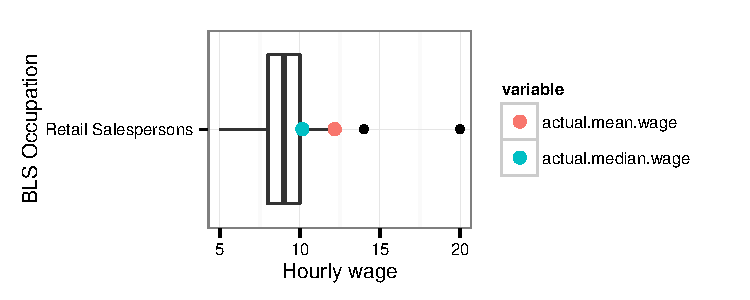
\includegraphics[width=\maxwidth]{figure/unnamed-chunk-21} 

}


\newpage\section{Secretaries and Administrative Assistants}\textbf{Occupation code:} 43-6010\newline\textbf{Typical entry education:} High school diploma or equivalent\newline\textbf{Detailed occupations:}\newline1. (43-6011)  \href{http://www.bls.gov/oes/current/oes436011.htm}{Executive Secretaries and Executive Administrative Assistants}\newline2. (43-6012)  \href{http://www.bls.gov/oes/current/oes436012.htm}{Legal Secretaries}\newline3. (43-6013)  \href{http://www.bls.gov/oes/current/oes436013.htm}{Medical Secretaries}\newline4. (43-6014)  \href{http://www.bls.gov/oes/current/oes436014.htm}{Secretaries and Administrative Assistants, Except Legal, Medical, and Executive}\newline% latex table generated in R 3.0.2 by xtable 1.7-1 package
% Sun Nov 24 09:11:37 2013
\begin{table}[ht]
\centering
{\footnotesize
\begin{tabular}{ll|rrr}
 \textbf{Variable} & \textbf{Levels} & $\mathbf{n}$ & $\mathbf{\%}$ & $\mathbf{\sum \%}$ \\ 
  \hline
know.job &  & 0 & 0.0 & 0.0 \\ 
   & Maybe & 2 & 6.7 & 6.7 \\ 
   & No & 0 & 0.0 & 6.7 \\ 
   & Yes & 28 & 93.3 & 100.0 \\ 
   \hline
 & all & 30 & 100.0 &  \\ 
   \hline
\hline
social.knowledge & 0 & 5 & 16.7 & 16.7 \\ 
   & 1 & 6 & 20.0 & 36.7 \\ 
   & 2 & 9 & 30.0 & 66.7 \\ 
   & 3-10 & 8 & 26.7 & 93.3 \\ 
   & 10-plus & 2 & 6.7 & 100.0 \\ 
   \hline
 & all & 30 & 100.0 &  \\ 
   \hline
\hline
Answer.volume\_trend &  & 0 & 0.0 & 0.0 \\ 
   & GoDown & 5 & 16.7 & 16.7 \\ 
   & GoUp & 11 & 36.7 & 53.3 \\ 
   & StayTheSame & 14 & 46.7 & 100.0 \\ 
   \hline
 & all & 30 & 100.0 &  \\ 
   \hline
\hline
Answer.wage\_trend &  & 0 & 0.0 & 0.0 \\ 
   & GoDown & 4 & 13.3 & 13.3 \\ 
   & GoUp & 15 & 50.0 & 63.3 \\ 
   & StayTheSame & 11 & 36.7 & 100.0 \\ 
   \hline
 & all & 30 & 100.0 &  \\ 
   \hline
\hline
\end{tabular}
}
\caption{Summary statistics, nominal variables (MTurk data)} 
\label{tab1:43-6010}
\end{table}
% latex table generated in R 3.0.2 by xtable 1.7-1 package
% Sun Nov 24 09:11:37 2013
\begin{table}[ht]
\centering
{\footnotesize
\begin{tabular}{lrrrrrrrrrr}
 \textbf{Variable} & $\mathbf{n}$ & \textbf{Min} & $\mathbf{q_1}$ & $\mathbf{\widetilde{x}}$ & $\mathbf{\bar{x}}$ & $\mathbf{q_3}$ & \textbf{Max} & $\mathbf{s}$ & \textbf{IQR} & \textbf{\#NA} \\ 
  \hline
wage & 30 & 10 & 12 & 14 & 13.7 & 15.5 & 20 & 2.9 & 3.5 & 0 \\ 
  \end{tabular}
}
\caption{Summary statistics, continuous variables (MTurk data)} 
\label{tab2:43-6010}
\end{table}


{\centering 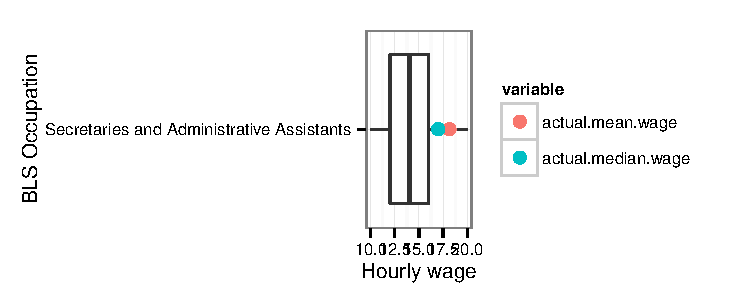
\includegraphics[width=\maxwidth]{figure/unnamed-chunk-22} 

}


\newpage\section{Fast Food and Counter Workers}\textbf{Occupation code:} 35-3020\newline\textbf{Typical entry education:} Less than high school\newline\textbf{Detailed occupations:}\newline1. (35-3021)  \href{http://www.bls.gov/oes/current/oes353021.htm}{Combined Food Preparation and Serving Workers, Including Fast Food}\newline2. (35-3022)  \href{http://www.bls.gov/oes/current/oes353022.htm}{Counter Attendants, Cafeteria, Food Concession, and Coffee Shop}\newline% latex table generated in R 3.0.2 by xtable 1.7-1 package
% Sun Nov 24 09:11:37 2013
\begin{table}[ht]
\centering
{\footnotesize
\begin{tabular}{ll|rrr}
 \textbf{Variable} & \textbf{Levels} & $\mathbf{n}$ & $\mathbf{\%}$ & $\mathbf{\sum \%}$ \\ 
  \hline
know.job &  & 0 & 0.0 & 0.0 \\ 
   & Maybe & 0 & 0.0 & 0.0 \\ 
   & No & 0 & 0.0 & 0.0 \\ 
   & Yes & 30 & 100.0 & 100.0 \\ 
   \hline
 & all & 30 & 100.0 &  \\ 
   \hline
\hline
social.knowledge & 0 & 12 & 40.0 & 40.0 \\ 
   & 1 & 5 & 16.7 & 56.7 \\ 
   & 2 & 6 & 20.0 & 76.7 \\ 
   & 3-10 & 5 & 16.7 & 93.3 \\ 
   & 10-plus & 2 & 6.7 & 100.0 \\ 
   \hline
 & all & 30 & 100.0 &  \\ 
   \hline
\hline
Answer.volume\_trend &  & 0 & 0.0 & 0.0 \\ 
   & GoDown & 4 & 13.3 & 13.3 \\ 
   & GoUp & 13 & 43.3 & 56.7 \\ 
   & StayTheSame & 13 & 43.3 & 100.0 \\ 
   \hline
 & all & 30 & 100.0 &  \\ 
   \hline
\hline
Answer.wage\_trend &  & 0 & 0.0 & 0.0 \\ 
   & GoDown & 1 & 3.3 & 3.3 \\ 
   & GoUp & 13 & 43.3 & 46.7 \\ 
   & StayTheSame & 16 & 53.3 & 100.0 \\ 
   \hline
 & all & 30 & 100.0 &  \\ 
   \hline
\hline
\end{tabular}
}
\caption{Summary statistics, nominal variables (MTurk data)} 
\label{tab1:35-3020}
\end{table}
% latex table generated in R 3.0.2 by xtable 1.7-1 package
% Sun Nov 24 09:11:37 2013
\begin{table}[ht]
\centering
{\footnotesize
\begin{tabular}{lrrrrrrrrrr}
 \textbf{Variable} & $\mathbf{n}$ & \textbf{Min} & $\mathbf{q_1}$ & $\mathbf{\widetilde{x}}$ & $\mathbf{\bar{x}}$ & $\mathbf{q_3}$ & \textbf{Max} & $\mathbf{s}$ & \textbf{IQR} & \textbf{\#NA} \\ 
  \hline
wage & 30 & 5 & 5 & 8 & 7 & 8 & 10 & 1.7 & 3 & 0 \\ 
  \end{tabular}
}
\caption{Summary statistics, continuous variables (MTurk data)} 
\label{tab2:35-3020}
\end{table}


{\centering 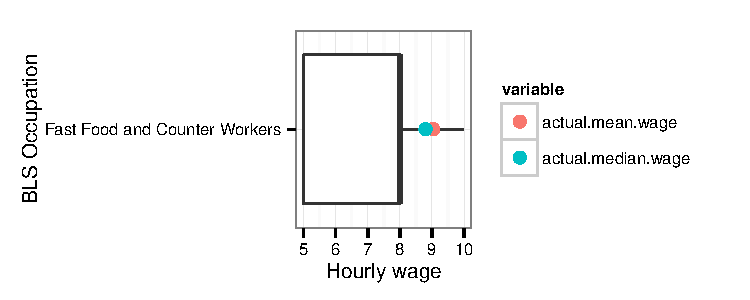
\includegraphics[width=\maxwidth]{figure/unnamed-chunk-23} 

}


\newpage\section{Cashiers}\textbf{Occupation code:} 41-2010\newline\textbf{Typical entry education:} Less than high school\newline\textbf{Detailed occupations:}\newline1. (41-2011)  \href{http://www.bls.gov/oes/current/oes412011.htm}{Cashiers}\newline2. (41-2012)  \href{http://www.bls.gov/oes/current/oes412012.htm}{Gaming Change Persons and Booth Cashiers}\newline% latex table generated in R 3.0.2 by xtable 1.7-1 package
% Sun Nov 24 09:11:38 2013
\begin{table}[ht]
\centering
{\footnotesize
\begin{tabular}{ll|rrr}
 \textbf{Variable} & \textbf{Levels} & $\mathbf{n}$ & $\mathbf{\%}$ & $\mathbf{\sum \%}$ \\ 
  \hline
know.job &  & 0 & 0.0 & 0.0 \\ 
   & Maybe & 0 & 0.0 & 0.0 \\ 
   & No & 0 & 0.0 & 0.0 \\ 
   & Yes & 30 & 100.0 & 100.0 \\ 
   \hline
 & all & 30 & 100.0 &  \\ 
   \hline
\hline
social.knowledge & 0 & 10 & 34.5 & 34.5 \\ 
   & 1 & 7 & 24.1 & 58.6 \\ 
   & 2 & 4 & 13.8 & 72.4 \\ 
   & 3-10 & 5 & 17.2 & 89.6 \\ 
   & 10-plus & 3 & 10.3 & 100.0 \\ 
   \hline
 & all & 29 & 100.0 &  \\ 
   \hline
\hline
Answer.volume\_trend &  & 0 & 0.0 & 0.0 \\ 
   & GoDown & 9 & 30.0 & 30.0 \\ 
   & GoUp & 9 & 30.0 & 60.0 \\ 
   & StayTheSame & 12 & 40.0 & 100.0 \\ 
   \hline
 & all & 30 & 100.0 &  \\ 
   \hline
\hline
Answer.wage\_trend &  & 0 & 0.0 & 0.0 \\ 
   & GoDown & 5 & 16.7 & 16.7 \\ 
   & GoUp & 13 & 43.3 & 60.0 \\ 
   & StayTheSame & 12 & 40.0 & 100.0 \\ 
   \hline
 & all & 30 & 100.0 &  \\ 
   \hline
\hline
\end{tabular}
}
\caption{Summary statistics, nominal variables (MTurk data)} 
\label{tab1:41-2010}
\end{table}
% latex table generated in R 3.0.2 by xtable 1.7-1 package
% Sun Nov 24 09:11:38 2013
\begin{table}[ht]
\centering
{\footnotesize
\begin{tabular}{lrrrrrrrrrr}
 \textbf{Variable} & $\mathbf{n}$ & \textbf{Min} & $\mathbf{q_1}$ & $\mathbf{\widetilde{x}}$ & $\mathbf{\bar{x}}$ & $\mathbf{q_3}$ & \textbf{Max} & $\mathbf{s}$ & \textbf{IQR} & \textbf{\#NA} \\ 
  \hline
wage & 30 & 5 & 8 & 9 & 9.0 & 10 & 16 & 2.0 & 2 & 0 \\ 
  \end{tabular}
}
\caption{Summary statistics, continuous variables (MTurk data)} 
\label{tab2:41-2010}
\end{table}


{\centering 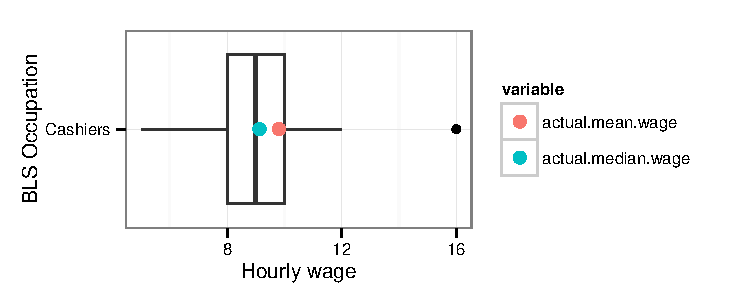
\includegraphics[width=\maxwidth]{figure/unnamed-chunk-24} 

}


\newpage\section{Laborers and Material Movers, Hand}\textbf{Occupation code:} 53-7060\newline\textbf{Typical entry education:} Less than high school\newline\textbf{Detailed occupations:}\newline1. (53-7061)  \href{http://www.bls.gov/oes/current/oes537061.htm}{Cleaners of Vehicles and Equipment}\newline2. (53-7062)  \href{http://www.bls.gov/oes/current/oes537062.htm}{Laborers and Freight, Stock, and Material Movers, Hand}\newline3. (53-7063)  \href{http://www.bls.gov/oes/current/oes537063.htm}{Machine Feeders and Offbearers}\newline4. (53-7064)  \href{http://www.bls.gov/oes/current/oes537064.htm}{Packers and Packagers, Hand}\newline% latex table generated in R 3.0.2 by xtable 1.7-1 package
% Sun Nov 24 09:11:38 2013
\begin{table}[ht]
\centering
{\footnotesize
\begin{tabular}{ll|rrr}
 \textbf{Variable} & \textbf{Levels} & $\mathbf{n}$ & $\mathbf{\%}$ & $\mathbf{\sum \%}$ \\ 
  \hline
know.job &  & 0 & 0.0 & 0.0 \\ 
   & Maybe & 4 & 13.3 & 13.3 \\ 
   & No & 2 & 6.7 & 20.0 \\ 
   & Yes & 24 & 80.0 & 100.0 \\ 
   \hline
 & all & 30 & 100.0 &  \\ 
   \hline
\hline
social.knowledge & 0 & 20 & 66.7 & 66.7 \\ 
   & 1 & 5 & 16.7 & 83.3 \\ 
   & 2 & 2 & 6.7 & 90.0 \\ 
   & 3-10 & 3 & 10.0 & 100.0 \\ 
   & 10-plus & 0 & 0.0 & 100.0 \\ 
   \hline
 & all & 30 & 100.0 &  \\ 
   \hline
\hline
Answer.volume\_trend &  & 0 & 0.0 & 0.0 \\ 
   & GoDown & 7 & 23.3 & 23.3 \\ 
   & GoUp & 11 & 36.7 & 60.0 \\ 
   & StayTheSame & 12 & 40.0 & 100.0 \\ 
   \hline
 & all & 30 & 100.0 &  \\ 
   \hline
\hline
Answer.wage\_trend &  & 0 & 0.0 & 0.0 \\ 
   & GoDown & 5 & 16.7 & 16.7 \\ 
   & GoUp & 9 & 30.0 & 46.7 \\ 
   & StayTheSame & 16 & 53.3 & 100.0 \\ 
   \hline
 & all & 30 & 100.0 &  \\ 
   \hline
\hline
\end{tabular}
}
\caption{Summary statistics, nominal variables (MTurk data)} 
\label{tab1:53-7060}
\end{table}
% latex table generated in R 3.0.2 by xtable 1.7-1 package
% Sun Nov 24 09:11:38 2013
\begin{table}[ht]
\centering
{\footnotesize
\begin{tabular}{lrrrrrrrrrr}
 \textbf{Variable} & $\mathbf{n}$ & \textbf{Min} & $\mathbf{q_1}$ & $\mathbf{\widetilde{x}}$ & $\mathbf{\bar{x}}$ & $\mathbf{q_3}$ & \textbf{Max} & $\mathbf{s}$ & \textbf{IQR} & \textbf{\#NA} \\ 
  \hline
wage & 30 & 8 & 10 & 11 & 12.5 & 14 & 24 & 4.0 & 4 & 0 \\ 
  \end{tabular}
}
\caption{Summary statistics, continuous variables (MTurk data)} 
\label{tab2:53-7060}
\end{table}


{\centering 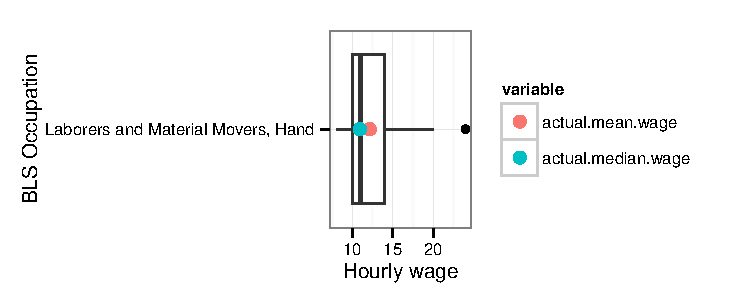
\includegraphics[width=\maxwidth]{figure/unnamed-chunk-25} 

}


\newpage\section{Building Cleaning Workers}\textbf{Occupation code:} 37-2010\newline\textbf{Typical entry education:} Less than high school\newline\textbf{Detailed occupations:}\newline1. (37-2011)  \href{http://www.bls.gov/oes/current/oes372011.htm}{Janitors and Cleaners, Except Maids and Housekeeping Cleaners}\newline2. (37-2012)  \href{http://www.bls.gov/oes/current/oes372012.htm}{Maids and Housekeeping Cleaners}\newline3. (37-2019)  \href{http://www.bls.gov/oes/current/oes372019.htm}{Building Cleaning Workers, All Other}\newline% latex table generated in R 3.0.2 by xtable 1.7-1 package
% Sun Nov 24 09:11:39 2013
\begin{table}[ht]
\centering
{\footnotesize
\begin{tabular}{ll|rrr}
 \textbf{Variable} & \textbf{Levels} & $\mathbf{n}$ & $\mathbf{\%}$ & $\mathbf{\sum \%}$ \\ 
  \hline
know.job &  & 0 & 0.0 & 0.0 \\ 
   & Maybe & 1 & 3.3 & 3.3 \\ 
   & No & 0 & 0.0 & 3.3 \\ 
   & Yes & 29 & 96.7 & 100.0 \\ 
   \hline
 & all & 30 & 100.0 &  \\ 
   \hline
\hline
social.knowledge & 0 & 17 & 56.7 & 56.7 \\ 
   & 1 & 10 & 33.3 & 90.0 \\ 
   & 2 & 2 & 6.7 & 96.7 \\ 
   & 3-10 & 1 & 3.3 & 100.0 \\ 
   & 10-plus & 0 & 0.0 & 100.0 \\ 
   \hline
 & all & 30 & 100.0 &  \\ 
   \hline
\hline
Answer.volume\_trend &  & 0 & 0.0 & 0.0 \\ 
   & GoDown & 2 & 6.7 & 6.7 \\ 
   & GoUp & 10 & 33.3 & 40.0 \\ 
   & StayTheSame & 18 & 60.0 & 100.0 \\ 
   \hline
 & all & 30 & 100.0 &  \\ 
   \hline
\hline
Answer.wage\_trend &  & 0 & 0.0 & 0.0 \\ 
   & GoDown & 4 & 13.3 & 13.3 \\ 
   & GoUp & 9 & 30.0 & 43.3 \\ 
   & StayTheSame & 17 & 56.7 & 100.0 \\ 
   \hline
 & all & 30 & 100.0 &  \\ 
   \hline
\hline
\end{tabular}
}
\caption{Summary statistics, nominal variables (MTurk data)} 
\label{tab1:37-2010}
\end{table}
% latex table generated in R 3.0.2 by xtable 1.7-1 package
% Sun Nov 24 09:11:39 2013
\begin{table}[ht]
\centering
{\footnotesize
\begin{tabular}{lrrrrrrrrrr}
 \textbf{Variable} & $\mathbf{n}$ & \textbf{Min} & $\mathbf{q_1}$ & $\mathbf{\widetilde{x}}$ & $\mathbf{\bar{x}}$ & $\mathbf{q_3}$ & \textbf{Max} & $\mathbf{s}$ & \textbf{IQR} & \textbf{\#NA} \\ 
  \hline
wage & 30 & 5 & 8 & 9.5 & 9.3 & 10 & 16 & 2.9 & 2 & 0 \\ 
  \end{tabular}
}
\caption{Summary statistics, continuous variables (MTurk data)} 
\label{tab2:37-2010}
\end{table}


{\centering 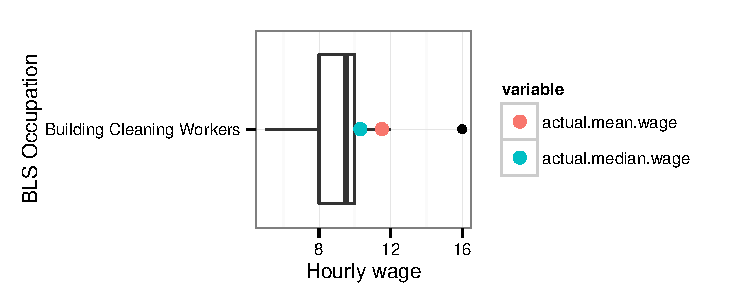
\includegraphics[width=\maxwidth]{figure/unnamed-chunk-26} 

}


\newpage\section{Office Clerks, General}\textbf{Occupation code:} 43-9060\newline\textbf{Typical entry education:} High school diploma or equivalent\newline\textbf{Detailed occupations:}\newline1. (43-9061)  \href{http://www.bls.gov/oes/current/oes439061.htm}{Office Clerks, General}\newline% latex table generated in R 3.0.2 by xtable 1.7-1 package
% Sun Nov 24 09:11:39 2013
\begin{table}[ht]
\centering
{\footnotesize
\begin{tabular}{ll|rrr}
 \textbf{Variable} & \textbf{Levels} & $\mathbf{n}$ & $\mathbf{\%}$ & $\mathbf{\sum \%}$ \\ 
  \hline
know.job &  & 0 & 0.0 & 0.0 \\ 
   & Maybe & 4 & 13.3 & 13.3 \\ 
   & No & 1 & 3.3 & 16.7 \\ 
   & Yes & 25 & 83.3 & 100.0 \\ 
   \hline
 & all & 30 & 100.0 &  \\ 
   \hline
\hline
social.knowledge & 0 & 10 & 33.3 & 33.3 \\ 
   & 1 & 11 & 36.7 & 70.0 \\ 
   & 2 & 5 & 16.7 & 86.7 \\ 
   & 3-10 & 4 & 13.3 & 100.0 \\ 
   & 10-plus & 0 & 0.0 & 100.0 \\ 
   \hline
 & all & 30 & 100.0 &  \\ 
   \hline
\hline
Answer.volume\_trend &  & 0 & 0.0 & 0.0 \\ 
   & GoDown & 5 & 16.7 & 16.7 \\ 
   & GoUp & 9 & 30.0 & 46.7 \\ 
   & StayTheSame & 16 & 53.3 & 100.0 \\ 
   \hline
 & all & 30 & 100.0 &  \\ 
   \hline
\hline
Answer.wage\_trend &  & 0 & 0.0 & 0.0 \\ 
   & GoDown & 4 & 13.3 & 13.3 \\ 
   & GoUp & 11 & 36.7 & 50.0 \\ 
   & StayTheSame & 15 & 50.0 & 100.0 \\ 
   \hline
 & all & 30 & 100.0 &  \\ 
   \hline
\hline
\end{tabular}
}
\caption{Summary statistics, nominal variables (MTurk data)} 
\label{tab1:43-9060}
\end{table}
% latex table generated in R 3.0.2 by xtable 1.7-1 package
% Sun Nov 24 09:11:39 2013
\begin{table}[ht]
\centering
{\footnotesize
\begin{tabular}{lrrrrrrrrrr}
 \textbf{Variable} & $\mathbf{n}$ & \textbf{Min} & $\mathbf{q_1}$ & $\mathbf{\widetilde{x}}$ & $\mathbf{\bar{x}}$ & $\mathbf{q_3}$ & \textbf{Max} & $\mathbf{s}$ & \textbf{IQR} & \textbf{\#NA} \\ 
  \hline
wage & 30 & 9 & 10 & 12 & 12.6 & 14 & 28 & 3.7 & 4 & 0 \\ 
  \end{tabular}
}
\caption{Summary statistics, continuous variables (MTurk data)} 
\label{tab2:43-9060}
\end{table}


{\centering 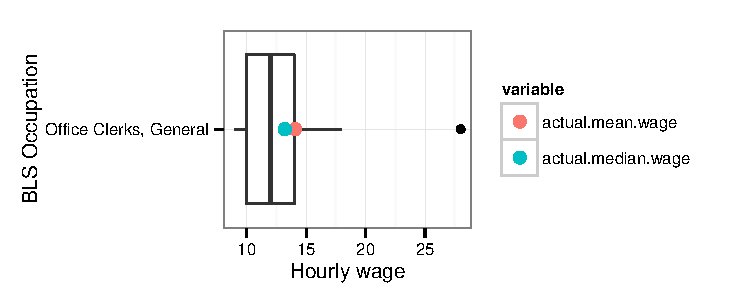
\includegraphics[width=\maxwidth]{figure/unnamed-chunk-27} 

}


\newpage\section{Driver/Sales Workers and Truck Drivers}\textbf{Occupation code:} 53-3030\newline\textbf{Typical entry education:} High school diploma or equivalent\newline\textbf{Detailed occupations:}\newline1. (53-3031)  \href{http://www.bls.gov/oes/current/oes533031.htm}{Driver/Sales Workers}\newline2. (53-3032)  \href{http://www.bls.gov/oes/current/oes533032.htm}{Heavy and Tractor-Trailer Truck Drivers}\newline3. (53-3033)  \href{http://www.bls.gov/oes/current/oes533033.htm}{Light Truck or Delivery Services Drivers}\newline% latex table generated in R 3.0.2 by xtable 1.7-1 package
% Sun Nov 24 09:11:39 2013
\begin{table}[ht]
\centering
{\footnotesize
\begin{tabular}{ll|rrr}
 \textbf{Variable} & \textbf{Levels} & $\mathbf{n}$ & $\mathbf{\%}$ & $\mathbf{\sum \%}$ \\ 
  \hline
know.job &  & 0 & 0.0 & 0.0 \\ 
   & Maybe & 0 & 0.0 & 0.0 \\ 
   & No & 0 & 0.0 & 0.0 \\ 
   & Yes & 30 & 100.0 & 100.0 \\ 
   \hline
 & all & 30 & 100.0 &  \\ 
   \hline
\hline
social.knowledge & 0 & 13 & 43.3 & 43.3 \\ 
   & 1 & 11 & 36.7 & 80.0 \\ 
   & 2 & 4 & 13.3 & 93.3 \\ 
   & 3-10 & 2 & 6.7 & 100.0 \\ 
   & 10-plus & 0 & 0.0 & 100.0 \\ 
   \hline
 & all & 30 & 100.0 &  \\ 
   \hline
\hline
Answer.volume\_trend &  & 0 & 0.0 & 0.0 \\ 
   & GoDown & 10 & 33.3 & 33.3 \\ 
   & GoUp & 9 & 30.0 & 63.3 \\ 
   & StayTheSame & 11 & 36.7 & 100.0 \\ 
   \hline
 & all & 30 & 100.0 &  \\ 
   \hline
\hline
Answer.wage\_trend &  & 0 & 0.0 & 0.0 \\ 
   & GoDown & 1 & 3.3 & 3.3 \\ 
   & GoUp & 16 & 53.3 & 56.7 \\ 
   & StayTheSame & 13 & 43.3 & 100.0 \\ 
   \hline
 & all & 30 & 100.0 &  \\ 
   \hline
\hline
\end{tabular}
}
\caption{Summary statistics, nominal variables (MTurk data)} 
\label{tab1:53-3030}
\end{table}
% latex table generated in R 3.0.2 by xtable 1.7-1 package
% Sun Nov 24 09:11:39 2013
\begin{table}[ht]
\centering
{\footnotesize
\begin{tabular}{lrrrrrrrrrr}
 \textbf{Variable} & $\mathbf{n}$ & \textbf{Min} & $\mathbf{q_1}$ & $\mathbf{\widetilde{x}}$ & $\mathbf{\bar{x}}$ & $\mathbf{q_3}$ & \textbf{Max} & $\mathbf{s}$ & \textbf{IQR} & \textbf{\#NA} \\ 
  \hline
wage & 30 & 9 & 12 & 16 & 17.6 & 23 & 36 & 6.3 & 11 & 0 \\ 
  \end{tabular}
}
\caption{Summary statistics, continuous variables (MTurk data)} 
\label{tab2:53-3030}
\end{table}


{\centering 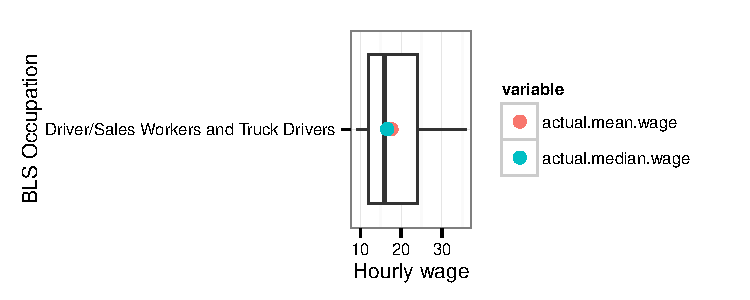
\includegraphics[width=\maxwidth]{figure/unnamed-chunk-28} 

}


\newpage\section{Registered Nurses}\textbf{Occupation code:} 29-1140\newline\textbf{Typical entry education:} Doctoral or professional degree\newline\textbf{Detailed occupations:}\newline1. (29-1141)  \href{http://www.bls.gov/oes/current/oes291141.htm}{Registered Nurses}\newline% latex table generated in R 3.0.2 by xtable 1.7-1 package
% Sun Nov 24 09:11:40 2013
\begin{table}[ht]
\centering
{\footnotesize
\begin{tabular}{ll|rrr}
 \textbf{Variable} & \textbf{Levels} & $\mathbf{n}$ & $\mathbf{\%}$ & $\mathbf{\sum \%}$ \\ 
  \hline
know.job &  & 0 & 0.0 & 0.0 \\ 
   & Maybe & 2 & 6.7 & 6.7 \\ 
   & No & 0 & 0.0 & 6.7 \\ 
   & Yes & 28 & 93.3 & 100.0 \\ 
   \hline
 & all & 30 & 100.0 &  \\ 
   \hline
\hline
social.knowledge & 0 & 7 & 23.3 & 23.3 \\ 
   & 1 & 9 & 30.0 & 53.3 \\ 
   & 2 & 7 & 23.3 & 76.7 \\ 
   & 3-10 & 5 & 16.7 & 93.3 \\ 
   & 10-plus & 2 & 6.7 & 100.0 \\ 
   \hline
 & all & 30 & 100.0 &  \\ 
   \hline
\hline
Answer.volume\_trend &  & 0 & 0.0 & 0.0 \\ 
   & GoDown & 0 & 0.0 & 0.0 \\ 
   & GoUp & 27 & 90.0 & 90.0 \\ 
   & StayTheSame & 3 & 10.0 & 100.0 \\ 
   \hline
 & all & 30 & 100.0 &  \\ 
   \hline
\hline
Answer.wage\_trend &  & 0 & 0.0 & 0.0 \\ 
   & GoDown & 1 & 3.3 & 3.3 \\ 
   & GoUp & 23 & 76.7 & 80.0 \\ 
   & StayTheSame & 6 & 20.0 & 100.0 \\ 
   \hline
 & all & 30 & 100.0 &  \\ 
   \hline
\hline
\end{tabular}
}
\caption{Summary statistics, nominal variables (MTurk data)} 
\label{tab1:29-1140}
\end{table}
% latex table generated in R 3.0.2 by xtable 1.7-1 package
% Sun Nov 24 09:11:40 2013
\begin{table}[ht]
\centering
{\footnotesize
\begin{tabular}{lrrrrrrrrrr}
 \textbf{Variable} & $\mathbf{n}$ & \textbf{Min} & $\mathbf{q_1}$ & $\mathbf{\widetilde{x}}$ & $\mathbf{\bar{x}}$ & $\mathbf{q_3}$ & \textbf{Max} & $\mathbf{s}$ & \textbf{IQR} & \textbf{\#NA} \\ 
  \hline
wage & 30 & 16 & 20 & 26 & 27.3 & 31 & 70 & 9.9 & 11 & 0 \\ 
  \end{tabular}
}
\caption{Summary statistics, continuous variables (MTurk data)} 
\label{tab2:29-1140}
\end{table}


{\centering 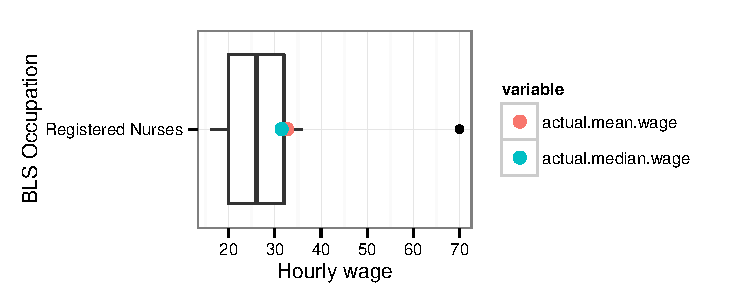
\includegraphics[width=\maxwidth]{figure/unnamed-chunk-29} 

}


\newpage\section{Nursing, Psychiatric, and Home Health Aides}\textbf{Occupation code:} 31-1010\newline\textbf{Typical entry education:} Less than high school\newline\textbf{Detailed occupations:}\newline1. (31-1011)  \href{http://www.bls.gov/oes/current/oes311011.htm}{Home Health Aides}\newline2. (31-1013)  \href{http://www.bls.gov/oes/current/oes311013.htm}{Psychiatric Aides}\newline3. (31-1014)  \href{http://www.bls.gov/oes/current/oes311014.htm}{Nursing Assistants}\newline4. (31-1015)  \href{http://www.bls.gov/oes/current/oes311015.htm}{Orderlies}\newline% latex table generated in R 3.0.2 by xtable 1.7-1 package
% Sun Nov 24 09:11:40 2013
\begin{table}[ht]
\centering
{\footnotesize
\begin{tabular}{ll|rrr}
 \textbf{Variable} & \textbf{Levels} & $\mathbf{n}$ & $\mathbf{\%}$ & $\mathbf{\sum \%}$ \\ 
  \hline
know.job &  & 0 & 0.0 & 0.0 \\ 
   & Maybe & 2 & 6.7 & 6.7 \\ 
   & No & 0 & 0.0 & 6.7 \\ 
   & Yes & 28 & 93.3 & 100.0 \\ 
   \hline
 & all & 30 & 100.0 &  \\ 
   \hline
\hline
social.knowledge & 0 & 12 & 40.0 & 40.0 \\ 
   & 1 & 10 & 33.3 & 73.3 \\ 
   & 2 & 5 & 16.7 & 90.0 \\ 
   & 3-10 & 3 & 10.0 & 100.0 \\ 
   & 10-plus & 0 & 0.0 & 100.0 \\ 
   \hline
 & all & 30 & 100.0 &  \\ 
   \hline
\hline
Answer.volume\_trend &  & 0 & 0.0 & 0.0 \\ 
   & GoDown & 3 & 10.0 & 10.0 \\ 
   & GoUp & 19 & 63.3 & 73.3 \\ 
   & StayTheSame & 8 & 26.7 & 100.0 \\ 
   \hline
 & all & 30 & 100.0 &  \\ 
   \hline
\hline
Answer.wage\_trend &  & 0 & 0.0 & 0.0 \\ 
   & GoDown & 1 & 3.3 & 3.3 \\ 
   & GoUp & 22 & 73.3 & 76.7 \\ 
   & StayTheSame & 7 & 23.3 & 100.0 \\ 
   \hline
 & all & 30 & 100.0 &  \\ 
   \hline
\hline
\end{tabular}
}
\caption{Summary statistics, nominal variables (MTurk data)} 
\label{tab1:31-1010}
\end{table}
% latex table generated in R 3.0.2 by xtable 1.7-1 package
% Sun Nov 24 09:11:40 2013
\begin{table}[ht]
\centering
{\footnotesize
\begin{tabular}{lrrrrrrrrrr}
 \textbf{Variable} & $\mathbf{n}$ & \textbf{Min} & $\mathbf{q_1}$ & $\mathbf{\widetilde{x}}$ & $\mathbf{\bar{x}}$ & $\mathbf{q_3}$ & \textbf{Max} & $\mathbf{s}$ & \textbf{IQR} & \textbf{\#NA} \\ 
  \hline
wage & 30 & 9 & 14.5 & 18 & 21.5 & 24 & 70 & 13.0 & 9.5 & 0 \\ 
  \end{tabular}
}
\caption{Summary statistics, continuous variables (MTurk data)} 
\label{tab2:31-1010}
\end{table}


{\centering 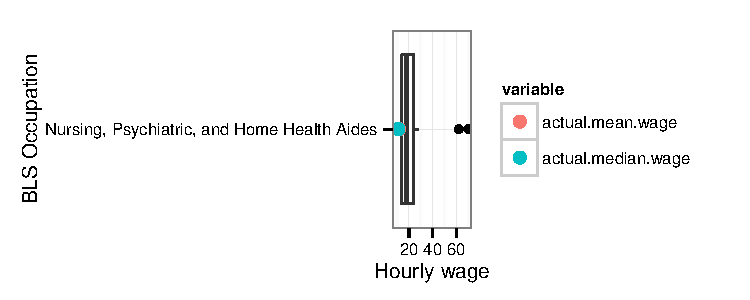
\includegraphics[width=\maxwidth]{figure/unnamed-chunk-210} 

}


\newpage\section{Waiters and Waitresses}\textbf{Occupation code:} 35-3030\newline\textbf{Typical entry education:} Less than high school\newline\textbf{Detailed occupations:}\newline1. (35-3031)  \href{http://www.bls.gov/oes/current/oes353031.htm}{Waiters and Waitresses}\newline% latex table generated in R 3.0.2 by xtable 1.7-1 package
% Sun Nov 24 09:11:41 2013
\begin{table}[ht]
\centering
{\footnotesize
\begin{tabular}{ll|rrr}
 \textbf{Variable} & \textbf{Levels} & $\mathbf{n}$ & $\mathbf{\%}$ & $\mathbf{\sum \%}$ \\ 
  \hline
know.job &  & 0 & 0.0 & 0.0 \\ 
   & Maybe & 0 & 0.0 & 0.0 \\ 
   & No & 0 & 0.0 & 0.0 \\ 
   & Yes & 30 & 100.0 & 100.0 \\ 
   \hline
 & all & 30 & 100.0 &  \\ 
   \hline
\hline
social.knowledge & 0 & 7 & 23.3 & 23.3 \\ 
   & 1 & 5 & 16.7 & 40.0 \\ 
   & 2 & 4 & 13.3 & 53.3 \\ 
   & 3-10 & 7 & 23.3 & 76.7 \\ 
   & 10-plus & 7 & 23.3 & 100.0 \\ 
   \hline
 & all & 30 & 100.0 &  \\ 
   \hline
\hline
Answer.volume\_trend &  & 0 & 0.0 & 0.0 \\ 
   & GoDown & 2 & 6.7 & 6.7 \\ 
   & GoUp & 17 & 56.7 & 63.3 \\ 
   & StayTheSame & 11 & 36.7 & 100.0 \\ 
   \hline
 & all & 30 & 100.0 &  \\ 
   \hline
\hline
Answer.wage\_trend &  & 0 & 0.0 & 0.0 \\ 
   & GoDown & 3 & 10.0 & 10.0 \\ 
   & GoUp & 14 & 46.7 & 56.7 \\ 
   & StayTheSame & 13 & 43.3 & 100.0 \\ 
   \hline
 & all & 30 & 100.0 &  \\ 
   \hline
\hline
\end{tabular}
}
\caption{Summary statistics, nominal variables (MTurk data)} 
\label{tab1:35-3030}
\end{table}
% latex table generated in R 3.0.2 by xtable 1.7-1 package
% Sun Nov 24 09:11:41 2013
\begin{table}[ht]
\centering
{\footnotesize
\begin{tabular}{lrrrrrrrrrr}
 \textbf{Variable} & $\mathbf{n}$ & \textbf{Min} & $\mathbf{q_1}$ & $\mathbf{\widetilde{x}}$ & $\mathbf{\bar{x}}$ & $\mathbf{q_3}$ & \textbf{Max} & $\mathbf{s}$ & \textbf{IQR} & \textbf{\#NA} \\ 
  \hline
wage & 30 & 5 & 5 & 6.5 & 8 & 9.8 & 20 & 3.9 & 4.8 & 0 \\ 
  \end{tabular}
}
\caption{Summary statistics, continuous variables (MTurk data)} 
\label{tab2:35-3030}
\end{table}


{\centering 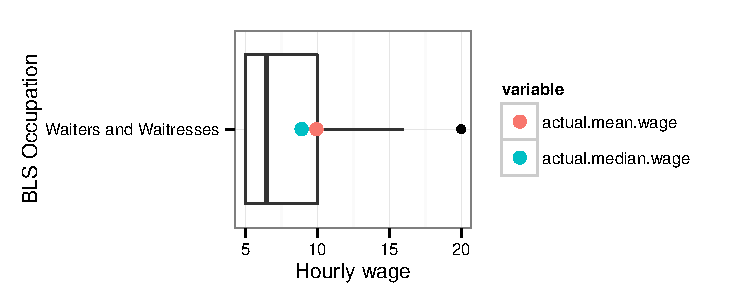
\includegraphics[width=\maxwidth]{figure/unnamed-chunk-211} 

}


\newpage\section{Customer Service Representatives}\textbf{Occupation code:} 43-4050\newline\textbf{Typical entry education:} High school diploma or equivalent\newline\textbf{Detailed occupations:}\newline1. (43-4051)  \href{http://www.bls.gov/oes/current/oes434051.htm}{Customer Service Representatives}\newline% latex table generated in R 3.0.2 by xtable 1.7-1 package
% Sun Nov 24 09:11:41 2013
\begin{table}[ht]
\centering
{\footnotesize
\begin{tabular}{ll|rrr}
 \textbf{Variable} & \textbf{Levels} & $\mathbf{n}$ & $\mathbf{\%}$ & $\mathbf{\sum \%}$ \\ 
  \hline
know.job &  & 0 & 0.0 & 0.0 \\ 
   & Maybe & 0 & 0.0 & 0.0 \\ 
   & No & 0 & 0.0 & 0.0 \\ 
   & Yes & 30 & 100.0 & 100.0 \\ 
   \hline
 & all & 30 & 100.0 &  \\ 
   \hline
\hline
social.knowledge & 0 & 10 & 33.3 & 33.3 \\ 
   & 1 & 5 & 16.7 & 50.0 \\ 
   & 2 & 2 & 6.7 & 56.7 \\ 
   & 3-10 & 8 & 26.7 & 83.3 \\ 
   & 10-plus & 5 & 16.7 & 100.0 \\ 
   \hline
 & all & 30 & 100.0 &  \\ 
   \hline
\hline
Answer.volume\_trend &  & 0 & 0.0 & 0.0 \\ 
   & GoDown & 6 & 20.0 & 20.0 \\ 
   & GoUp & 12 & 40.0 & 60.0 \\ 
   & StayTheSame & 12 & 40.0 & 100.0 \\ 
   \hline
 & all & 30 & 100.0 &  \\ 
   \hline
\hline
Answer.wage\_trend &  & 0 & 0.0 & 0.0 \\ 
   & GoDown & 4 & 13.3 & 13.3 \\ 
   & GoUp & 12 & 40.0 & 53.3 \\ 
   & StayTheSame & 14 & 46.7 & 100.0 \\ 
   \hline
 & all & 30 & 100.0 &  \\ 
   \hline
\hline
\end{tabular}
}
\caption{Summary statistics, nominal variables (MTurk data)} 
\label{tab1:43-4050}
\end{table}
% latex table generated in R 3.0.2 by xtable 1.7-1 package
% Sun Nov 24 09:11:41 2013
\begin{table}[ht]
\centering
{\footnotesize
\begin{tabular}{lrrrrrrrrrr}
 \textbf{Variable} & $\mathbf{n}$ & \textbf{Min} & $\mathbf{q_1}$ & $\mathbf{\widetilde{x}}$ & $\mathbf{\bar{x}}$ & $\mathbf{q_3}$ & \textbf{Max} & $\mathbf{s}$ & \textbf{IQR} & \textbf{\#NA} \\ 
  \hline
wage & 30 & 8 & 10 & 10 & 11.2 & 12 & 16 & 2.2 & 2 & 0 \\ 
  \end{tabular}
}
\caption{Summary statistics, continuous variables (MTurk data)} 
\label{tab2:43-4050}
\end{table}


{\centering 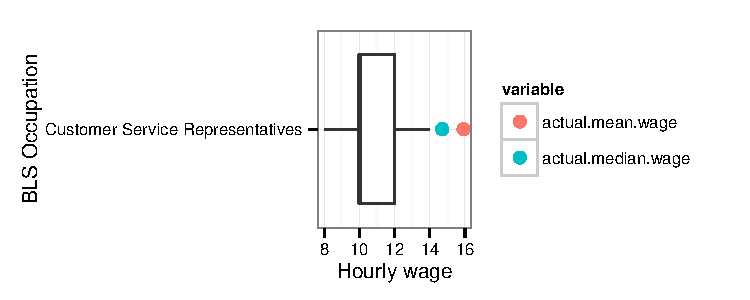
\includegraphics[width=\maxwidth]{figure/unnamed-chunk-212} 

}


\newpage\section{Cooks}\textbf{Occupation code:} 35-2010\newline\textbf{Typical entry education:} Less than high school\newline\textbf{Detailed occupations:}\newline1. (35-2011)  \href{http://www.bls.gov/oes/current/oes352011.htm}{Cooks, Fast Food}\newline2. (35-2012)  \href{http://www.bls.gov/oes/current/oes352012.htm}{Cooks, Institution and Cafeteria}\newline3. (35-2013)  \href{http://www.bls.gov/oes/current/oes352013.htm}{Cooks, Private Household}\newline4. (35-2014)  \href{http://www.bls.gov/oes/current/oes352014.htm}{Cooks, Restaurant}\newline5. (35-2015)  \href{http://www.bls.gov/oes/current/oes352015.htm}{Cooks, Short Order}\newline6. (35-2019)  \href{http://www.bls.gov/oes/current/oes352019.htm}{Cooks, All Other}\newline% latex table generated in R 3.0.2 by xtable 1.7-1 package
% Sun Nov 24 09:11:42 2013
\begin{table}[ht]
\centering
{\footnotesize
\begin{tabular}{ll|rrr}
 \textbf{Variable} & \textbf{Levels} & $\mathbf{n}$ & $\mathbf{\%}$ & $\mathbf{\sum \%}$ \\ 
  \hline
know.job &  & 0 & 0.0 & 0.0 \\ 
   & Maybe & 0 & 0.0 & 0.0 \\ 
   & No & 0 & 0.0 & 0.0 \\ 
   & Yes & 30 & 100.0 & 100.0 \\ 
   \hline
 & all & 30 & 100.0 &  \\ 
   \hline
\hline
social.knowledge & 0 & 8 & 26.7 & 26.7 \\ 
   & 1 & 7 & 23.3 & 50.0 \\ 
   & 2 & 10 & 33.3 & 83.3 \\ 
   & 3-10 & 5 & 16.7 & 100.0 \\ 
   & 10-plus & 0 & 0.0 & 100.0 \\ 
   \hline
 & all & 30 & 100.0 &  \\ 
   \hline
\hline
Answer.volume\_trend &  & 0 & 0.0 & 0.0 \\ 
   & GoDown & 3 & 10.0 & 10.0 \\ 
   & GoUp & 17 & 56.7 & 66.7 \\ 
   & StayTheSame & 10 & 33.3 & 100.0 \\ 
   \hline
 & all & 30 & 100.0 &  \\ 
   \hline
\hline
Answer.wage\_trend &  & 1 & 3.3 & 3.3 \\ 
   & GoDown & 2 & 6.7 & 10.0 \\ 
   & GoUp & 17 & 56.7 & 66.7 \\ 
   & StayTheSame & 10 & 33.3 & 100.0 \\ 
   \hline
 & all & 30 & 100.0 &  \\ 
   \hline
\hline
\end{tabular}
}
\caption{Summary statistics, nominal variables (MTurk data)} 
\label{tab1:35-2010}
\end{table}
% latex table generated in R 3.0.2 by xtable 1.7-1 package
% Sun Nov 24 09:11:42 2013
\begin{table}[ht]
\centering
{\footnotesize
\begin{tabular}{lrrrrrrrrrr}
 \textbf{Variable} & $\mathbf{n}$ & \textbf{Min} & $\mathbf{q_1}$ & $\mathbf{\widetilde{x}}$ & $\mathbf{\bar{x}}$ & $\mathbf{q_3}$ & \textbf{Max} & $\mathbf{s}$ & \textbf{IQR} & \textbf{\#NA} \\ 
  \hline
wage & 30 & 8 & 10 & 12 & 13.2 & 16 & 20 & 3.8 & 6 & 0 \\ 
  \end{tabular}
}
\caption{Summary statistics, continuous variables (MTurk data)} 
\label{tab2:35-2010}
\end{table}


{\centering 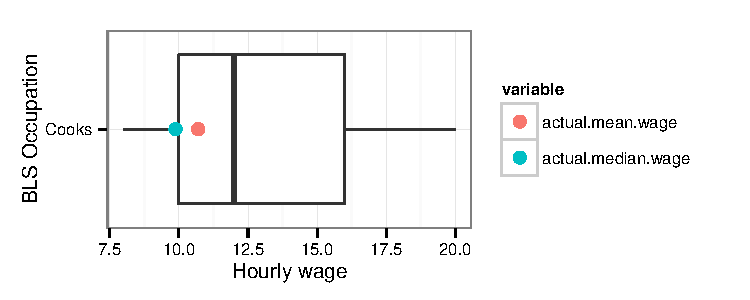
\includegraphics[width=\maxwidth]{figure/unnamed-chunk-213} 

}


\newpage\section{Elementary and Middle School Teachers}\textbf{Occupation code:} 25-2020\newline\textbf{Typical entry education:} Bachelor's degree\newline\textbf{Detailed occupations:}\newline1. (25-2021)  \href{http://www.bls.gov/oes/current/oes252021.htm}{Elementary School Teachers, Except Special Education}\newline2. (25-2022)  \href{http://www.bls.gov/oes/current/oes252022.htm}{Middle School Teachers, Except Special and Career/Technical Education}\newline3. (25-2023)  \href{http://www.bls.gov/oes/current/oes252023.htm}{Career/Technical Education Teachers, Middle School}\newline% latex table generated in R 3.0.2 by xtable 1.7-1 package
% Sun Nov 24 09:11:42 2013
\begin{table}[ht]
\centering
{\footnotesize
\begin{tabular}{ll|rrr}
 \textbf{Variable} & \textbf{Levels} & $\mathbf{n}$ & $\mathbf{\%}$ & $\mathbf{\sum \%}$ \\ 
  \hline
know.job &  & 0 & 0.0 & 0.0 \\ 
   & Maybe & 1 & 3.3 & 3.3 \\ 
   & No & 0 & 0.0 & 3.3 \\ 
   & Yes & 29 & 96.7 & 100.0 \\ 
   \hline
 & all & 30 & 100.0 &  \\ 
   \hline
\hline
social.knowledge & 0 & 3 & 10.0 & 10.0 \\ 
   & 1 & 12 & 40.0 & 50.0 \\ 
   & 2 & 5 & 16.7 & 66.7 \\ 
   & 3-10 & 6 & 20.0 & 86.7 \\ 
   & 10-plus & 4 & 13.3 & 100.0 \\ 
   \hline
 & all & 30 & 100.0 &  \\ 
   \hline
\hline
Answer.volume\_trend &  & 0 & 0.0 & 0.0 \\ 
   & GoDown & 3 & 10.0 & 10.0 \\ 
   & GoUp & 21 & 70.0 & 80.0 \\ 
   & StayTheSame & 6 & 20.0 & 100.0 \\ 
   \hline
 & all & 30 & 100.0 &  \\ 
   \hline
\hline
Answer.wage\_trend &  & 0 & 0.0 & 0.0 \\ 
   & GoDown & 5 & 16.7 & 16.7 \\ 
   & GoUp & 19 & 63.3 & 80.0 \\ 
   & StayTheSame & 6 & 20.0 & 100.0 \\ 
   \hline
 & all & 30 & 100.0 &  \\ 
   \hline
\hline
\end{tabular}
}
\caption{Summary statistics, nominal variables (MTurk data)} 
\label{tab1:25-2020}
\end{table}
% latex table generated in R 3.0.2 by xtable 1.7-1 package
% Sun Nov 24 09:11:42 2013
\begin{table}[ht]
\centering
{\footnotesize
\begin{tabular}{lrrrrrrrrrr}
 \textbf{Variable} & $\mathbf{n}$ & \textbf{Min} & $\mathbf{q_1}$ & $\mathbf{\widetilde{x}}$ & $\mathbf{\bar{x}}$ & $\mathbf{q_3}$ & \textbf{Max} & $\mathbf{s}$ & \textbf{IQR} & \textbf{\#NA} \\ 
  \hline
wage & 30 & 12 & 16 & 18 & 19.9 & 23 & 50 & 7.6 & 7 & 0 \\ 
  \end{tabular}
}
\caption{Summary statistics, continuous variables (MTurk data)} 
\label{tab2:25-2020}
\end{table}


{\centering 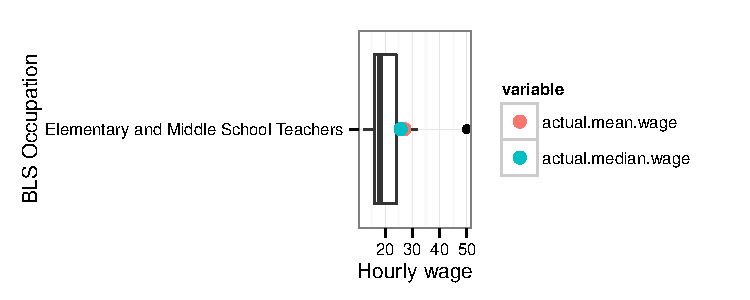
\includegraphics[width=\maxwidth]{figure/unnamed-chunk-214} 

}


\newpage\section{General and Operations Managers}\textbf{Occupation code:} 11-1020\newline\textbf{Typical entry education:} Associate's degree\newline\textbf{Detailed occupations:}\newline1. (11-1021)  \href{http://www.bls.gov/oes/current/oes111021.htm}{General and Operations Managers}\newline% latex table generated in R 3.0.2 by xtable 1.7-1 package
% Sun Nov 24 09:11:42 2013
\begin{table}[ht]
\centering
{\footnotesize
\begin{tabular}{ll|rrr}
 \textbf{Variable} & \textbf{Levels} & $\mathbf{n}$ & $\mathbf{\%}$ & $\mathbf{\sum \%}$ \\ 
  \hline
know.job &  & 0 & 0.0 & 0.0 \\ 
   & Maybe & 7 & 23.3 & 23.3 \\ 
   & No & 2 & 6.7 & 30.0 \\ 
   & Yes & 21 & 70.0 & 100.0 \\ 
   \hline
 & all & 30 & 100.0 &  \\ 
   \hline
\hline
social.knowledge & 0 & 14 & 46.7 & 46.7 \\ 
   & 1 & 12 & 40.0 & 86.7 \\ 
   & 2 & 1 & 3.3 & 90.0 \\ 
   & 3-10 & 3 & 10.0 & 100.0 \\ 
   & 10-plus & 0 & 0.0 & 100.0 \\ 
   \hline
 & all & 30 & 100.0 &  \\ 
   \hline
\hline
Answer.volume\_trend &  & 0 & 0.0 & 0.0 \\ 
   & GoDown & 3 & 10.0 & 10.0 \\ 
   & GoUp & 8 & 26.7 & 36.7 \\ 
   & StayTheSame & 19 & 63.3 & 100.0 \\ 
   \hline
 & all & 30 & 100.0 &  \\ 
   \hline
\hline
Answer.wage\_trend &  & 0 & 0.0 & 0.0 \\ 
   & GoDown & 1 & 3.3 & 3.3 \\ 
   & GoUp & 15 & 50.0 & 53.3 \\ 
   & StayTheSame & 14 & 46.7 & 100.0 \\ 
   \hline
 & all & 30 & 100.0 &  \\ 
   \hline
\hline
\end{tabular}
}
\caption{Summary statistics, nominal variables (MTurk data)} 
\label{tab1:11-1020}
\end{table}
% latex table generated in R 3.0.2 by xtable 1.7-1 package
% Sun Nov 24 09:11:42 2013
\begin{table}[ht]
\centering
{\footnotesize
\begin{tabular}{lrrrrrrrrrr}
 \textbf{Variable} & $\mathbf{n}$ & \textbf{Min} & $\mathbf{q_1}$ & $\mathbf{\widetilde{x}}$ & $\mathbf{\bar{x}}$ & $\mathbf{q_3}$ & \textbf{Max} & $\mathbf{s}$ & \textbf{IQR} & \textbf{\#NA} \\ 
  \hline
wage & 30 & 12 & 18 & 20 & 22.1 & 24 & 36 & 6.0 & 6 & 0 \\ 
  \end{tabular}
}
\caption{Summary statistics, continuous variables (MTurk data)} 
\label{tab2:11-1020}
\end{table}


{\centering 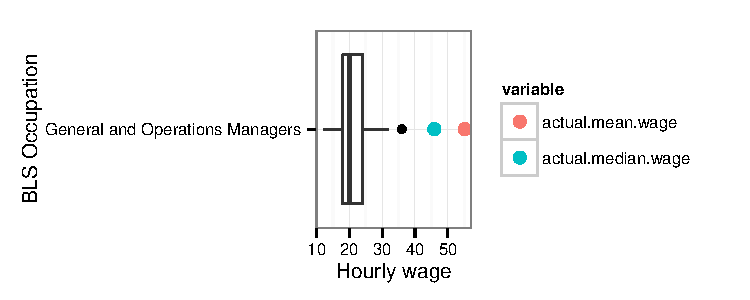
\includegraphics[width=\maxwidth]{figure/unnamed-chunk-215} 

}


\newpage\section{Stock Clerks and Order Fillers}\textbf{Occupation code:} 43-5080\newline\textbf{Typical entry education:} Less than high school\newline\textbf{Detailed occupations:}\newline1. (43-5081)  \href{http://www.bls.gov/oes/current/oes435081.htm}{Stock Clerks and Order Fillers}\newline% latex table generated in R 3.0.2 by xtable 1.7-1 package
% Sun Nov 24 09:11:43 2013
\begin{table}[ht]
\centering
{\footnotesize
\begin{tabular}{ll|rrr}
 \textbf{Variable} & \textbf{Levels} & $\mathbf{n}$ & $\mathbf{\%}$ & $\mathbf{\sum \%}$ \\ 
  \hline
know.job &  & 0 & 0.0 & 0.0 \\ 
   & Maybe & 4 & 13.3 & 13.3 \\ 
   & No & 1 & 3.3 & 16.7 \\ 
   & Yes & 25 & 83.3 & 100.0 \\ 
   \hline
 & all & 30 & 100.0 &  \\ 
   \hline
\hline
social.knowledge & 0 & 14 & 48.3 & 48.3 \\ 
   & 1 & 8 & 27.6 & 75.9 \\ 
   & 2 & 3 & 10.3 & 86.2 \\ 
   & 3-10 & 1 & 3.5 & 89.7 \\ 
   & 10-plus & 3 & 10.3 & 100.0 \\ 
   \hline
 & all & 29 & 100.0 &  \\ 
   \hline
\hline
Answer.volume\_trend &  & 0 & 0.0 & 0.0 \\ 
   & GoDown & 4 & 13.3 & 13.3 \\ 
   & GoUp & 14 & 46.7 & 60.0 \\ 
   & StayTheSame & 12 & 40.0 & 100.0 \\ 
   \hline
 & all & 30 & 100.0 &  \\ 
   \hline
\hline
Answer.wage\_trend &  & 0 & 0.0 & 0.0 \\ 
   & GoDown & 4 & 13.3 & 13.3 \\ 
   & GoUp & 12 & 40.0 & 53.3 \\ 
   & StayTheSame & 14 & 46.7 & 100.0 \\ 
   \hline
 & all & 30 & 100.0 &  \\ 
   \hline
\hline
\end{tabular}
}
\caption{Summary statistics, nominal variables (MTurk data)} 
\label{tab1:43-5080}
\end{table}
% latex table generated in R 3.0.2 by xtable 1.7-1 package
% Sun Nov 24 09:11:43 2013
\begin{table}[ht]
\centering
{\footnotesize
\begin{tabular}{lrrrrrrrrrr}
 \textbf{Variable} & $\mathbf{n}$ & \textbf{Min} & $\mathbf{q_1}$ & $\mathbf{\widetilde{x}}$ & $\mathbf{\bar{x}}$ & $\mathbf{q_3}$ & \textbf{Max} & $\mathbf{s}$ & \textbf{IQR} & \textbf{\#NA} \\ 
  \hline
wage & 30 & 5 & 8 & 10 & 9.5 & 10 & 16 & 2.6 & 2 & 0 \\ 
  \end{tabular}
}
\caption{Summary statistics, continuous variables (MTurk data)} 
\label{tab2:43-5080}
\end{table}


{\centering 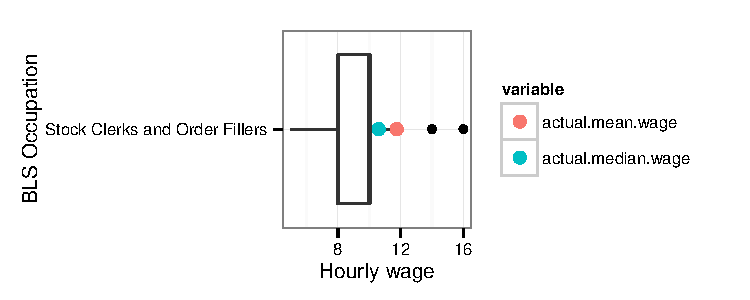
\includegraphics[width=\maxwidth]{figure/unnamed-chunk-216} 

}


\newpage\section{Sales Representatives, Wholesale and Manufacturing}\textbf{Occupation code:} 41-4010\newline\textbf{Typical entry education:} High school diploma or equivalent\newline\textbf{Detailed occupations:}\newline1. (41-4011)  \href{http://www.bls.gov/oes/current/oes414011.htm}{Sales Representatives, Wholesale and Manufacturing, Technical and Scientific Products}\newline2. (41-4012)  \href{http://www.bls.gov/oes/current/oes414012.htm}{Sales Representatives, Wholesale and Manufacturing, Except Technical and Scientific Products}\newline% latex table generated in R 3.0.2 by xtable 1.7-1 package
% Sun Nov 24 09:11:43 2013
\begin{table}[ht]
\centering
{\footnotesize
\begin{tabular}{ll|rrr}
 \textbf{Variable} & \textbf{Levels} & $\mathbf{n}$ & $\mathbf{\%}$ & $\mathbf{\sum \%}$ \\ 
  \hline
know.job &  & 0 & 0.0 & 0.0 \\ 
   & Maybe & 6 & 20.0 & 20.0 \\ 
   & No & 0 & 0.0 & 20.0 \\ 
   & Yes & 24 & 80.0 & 100.0 \\ 
   \hline
 & all & 30 & 100.0 &  \\ 
   \hline
\hline
social.knowledge & 0 & 11 & 36.7 & 36.7 \\ 
   & 1 & 7 & 23.3 & 60.0 \\ 
   & 2 & 6 & 20.0 & 80.0 \\ 
   & 3-10 & 4 & 13.3 & 93.3 \\ 
   & 10-plus & 2 & 6.7 & 100.0 \\ 
   \hline
 & all & 30 & 100.0 &  \\ 
   \hline
\hline
Answer.volume\_trend &  & 0 & 0.0 & 0.0 \\ 
   & GoDown & 9 & 30.0 & 30.0 \\ 
   & GoUp & 9 & 30.0 & 60.0 \\ 
   & StayTheSame & 12 & 40.0 & 100.0 \\ 
   \hline
 & all & 30 & 100.0 &  \\ 
   \hline
\hline
Answer.wage\_trend &  & 0 & 0.0 & 0.0 \\ 
   & GoDown & 2 & 6.7 & 6.7 \\ 
   & GoUp & 13 & 43.3 & 50.0 \\ 
   & StayTheSame & 15 & 50.0 & 100.0 \\ 
   \hline
 & all & 30 & 100.0 &  \\ 
   \hline
\hline
\end{tabular}
}
\caption{Summary statistics, nominal variables (MTurk data)} 
\label{tab1:41-4010}
\end{table}
% latex table generated in R 3.0.2 by xtable 1.7-1 package
% Sun Nov 24 09:11:43 2013
\begin{table}[ht]
\centering
{\footnotesize
\begin{tabular}{lrrrrrrrrrr}
 \textbf{Variable} & $\mathbf{n}$ & \textbf{Min} & $\mathbf{q_1}$ & $\mathbf{\widetilde{x}}$ & $\mathbf{\bar{x}}$ & $\mathbf{q_3}$ & \textbf{Max} & $\mathbf{s}$ & \textbf{IQR} & \textbf{\#NA} \\ 
  \hline
wage & 30 & 9 & 14 & 19 & 19.6 & 23 & 50 & 9.0 & 9 & 0 \\ 
  \end{tabular}
}
\caption{Summary statistics, continuous variables (MTurk data)} 
\label{tab2:41-4010}
\end{table}


{\centering 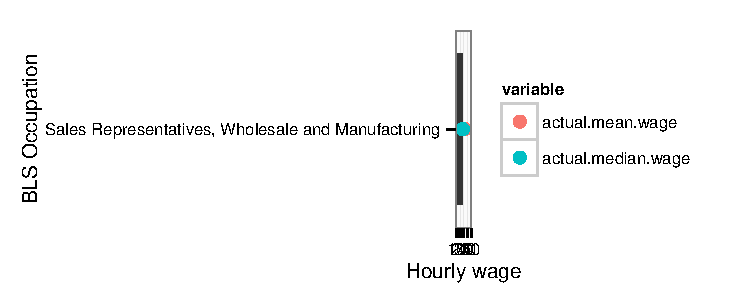
\includegraphics[width=\maxwidth]{figure/unnamed-chunk-217} 

}


\newpage\section{Bookkeeping, Accounting, and Auditing Clerks}\textbf{Occupation code:} 43-3030\newline\textbf{Typical entry education:} High school diploma or equivalent\newline\textbf{Detailed occupations:}\newline1. (43-3031)  \href{http://www.bls.gov/oes/current/oes433031.htm}{Bookkeeping, Accounting, and Auditing Clerks}\newline% latex table generated in R 3.0.2 by xtable 1.7-1 package
% Sun Nov 24 09:11:44 2013
\begin{table}[ht]
\centering
{\footnotesize
\begin{tabular}{ll|rrr}
 \textbf{Variable} & \textbf{Levels} & $\mathbf{n}$ & $\mathbf{\%}$ & $\mathbf{\sum \%}$ \\ 
  \hline
know.job &  & 0 & 0.0 & 0.0 \\ 
   & Maybe & 7 & 23.3 & 23.3 \\ 
   & No & 0 & 0.0 & 23.3 \\ 
   & Yes & 23 & 76.7 & 100.0 \\ 
   \hline
 & all & 30 & 100.0 &  \\ 
   \hline
\hline
social.knowledge & 0 & 15 & 50.0 & 50.0 \\ 
   & 1 & 5 & 16.7 & 66.7 \\ 
   & 2 & 6 & 20.0 & 86.7 \\ 
   & 3-10 & 4 & 13.3 & 100.0 \\ 
   & 10-plus & 0 & 0.0 & 100.0 \\ 
   \hline
 & all & 30 & 100.0 &  \\ 
   \hline
\hline
Answer.volume\_trend &  & 0 & 0.0 & 0.0 \\ 
   & GoDown & 8 & 26.7 & 26.7 \\ 
   & GoUp & 12 & 40.0 & 66.7 \\ 
   & StayTheSame & 10 & 33.3 & 100.0 \\ 
   \hline
 & all & 30 & 100.0 &  \\ 
   \hline
\hline
Answer.wage\_trend &  & 0 & 0.0 & 0.0 \\ 
   & GoDown & 2 & 6.7 & 6.7 \\ 
   & GoUp & 15 & 50.0 & 56.7 \\ 
   & StayTheSame & 13 & 43.3 & 100.0 \\ 
   \hline
 & all & 30 & 100.0 &  \\ 
   \hline
\hline
\end{tabular}
}
\caption{Summary statistics, nominal variables (MTurk data)} 
\label{tab1:43-3030}
\end{table}
% latex table generated in R 3.0.2 by xtable 1.7-1 package
% Sun Nov 24 09:11:44 2013
\begin{table}[ht]
\centering
{\footnotesize
\begin{tabular}{lrrrrrrrrrr}
 \textbf{Variable} & $\mathbf{n}$ & \textbf{Min} & $\mathbf{q_1}$ & $\mathbf{\widetilde{x}}$ & $\mathbf{\bar{x}}$ & $\mathbf{q_3}$ & \textbf{Max} & $\mathbf{s}$ & \textbf{IQR} & \textbf{\#NA} \\ 
  \hline
wage & 30 & 10 & 14 & 18 & 22 & 24 & 54 & 12.6 & 10 & 0 \\ 
  \end{tabular}
}
\caption{Summary statistics, continuous variables (MTurk data)} 
\label{tab2:43-3030}
\end{table}


{\centering 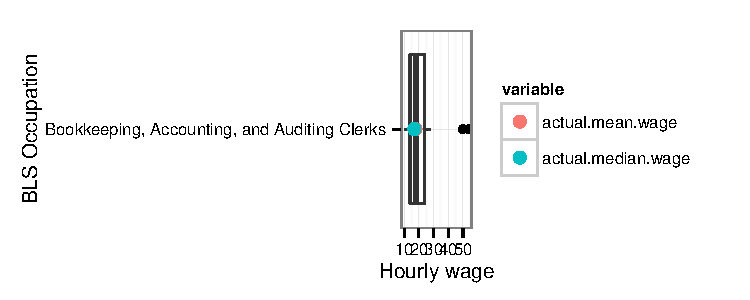
\includegraphics[width=\maxwidth]{figure/unnamed-chunk-218} 

}


\newpage\section{First-Line Supervisors of Sales Workers}\textbf{Occupation code:} 41-1010\newline\textbf{Typical entry education:} High school diploma or equivalent\newline\textbf{Detailed occupations:}\newline1. (41-1011)  \href{http://www.bls.gov/oes/current/oes411011.htm}{First-Line Supervisors of Retail Sales Workers}\newline2. (41-1012)  \href{http://www.bls.gov/oes/current/oes411012.htm}{First-Line Supervisors of Non-Retail Sales Workers}\newline% latex table generated in R 3.0.2 by xtable 1.7-1 package
% Sun Nov 24 09:11:44 2013
\begin{table}[ht]
\centering
{\footnotesize
\begin{tabular}{ll|rrr}
 \textbf{Variable} & \textbf{Levels} & $\mathbf{n}$ & $\mathbf{\%}$ & $\mathbf{\sum \%}$ \\ 
  \hline
know.job &  & 1 & 3.3 & 3.3 \\ 
   & Maybe & 6 & 20.0 & 23.3 \\ 
   & No & 0 & 0.0 & 23.3 \\ 
   & Yes & 23 & 76.7 & 100.0 \\ 
   \hline
 & all & 30 & 100.0 &  \\ 
   \hline
\hline
social.knowledge & 0 & 14 & 46.7 & 46.7 \\ 
   & 1 & 11 & 36.7 & 83.3 \\ 
   & 2 & 2 & 6.7 & 90.0 \\ 
   & 3-10 & 3 & 10.0 & 100.0 \\ 
   & 10-plus & 0 & 0.0 & 100.0 \\ 
   \hline
 & all & 30 & 100.0 &  \\ 
   \hline
\hline
Answer.volume\_trend &  & 0 & 0.0 & 0.0 \\ 
   & GoDown & 6 & 20.0 & 20.0 \\ 
   & GoUp & 9 & 30.0 & 50.0 \\ 
   & StayTheSame & 15 & 50.0 & 100.0 \\ 
   \hline
 & all & 30 & 100.0 &  \\ 
   \hline
\hline
Answer.wage\_trend &  & 0 & 0.0 & 0.0 \\ 
   & GoDown & 5 & 16.7 & 16.7 \\ 
   & GoUp & 13 & 43.3 & 60.0 \\ 
   & StayTheSame & 12 & 40.0 & 100.0 \\ 
   \hline
 & all & 30 & 100.0 &  \\ 
   \hline
\hline
\end{tabular}
}
\caption{Summary statistics, nominal variables (MTurk data)} 
\label{tab1:41-1010}
\end{table}
% latex table generated in R 3.0.2 by xtable 1.7-1 package
% Sun Nov 24 09:11:44 2013
\begin{table}[ht]
\centering
{\footnotesize
\begin{tabular}{lrrrrrrrrrr}
 \textbf{Variable} & $\mathbf{n}$ & \textbf{Min} & $\mathbf{q_1}$ & $\mathbf{\widetilde{x}}$ & $\mathbf{\bar{x}}$ & $\mathbf{q_3}$ & \textbf{Max} & $\mathbf{s}$ & \textbf{IQR} & \textbf{\#NA} \\ 
  \hline
wage & 30 & 10 & 14 & 16 & 16 & 19.5 & 24 & 3.5 & 5.5 & 0 \\ 
  \end{tabular}
}
\caption{Summary statistics, continuous variables (MTurk data)} 
\label{tab2:41-1010}
\end{table}


{\centering 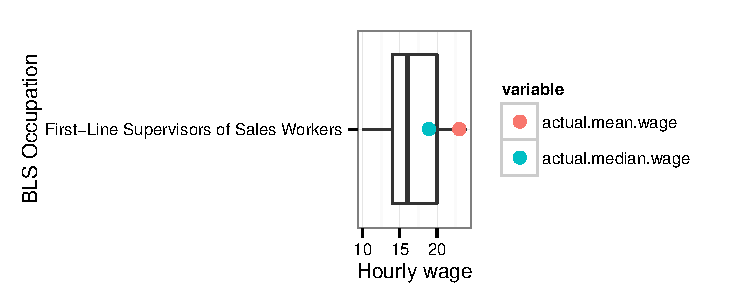
\includegraphics[width=\maxwidth]{figure/unnamed-chunk-219} 

}


\newpage\section{Software Developers and Programmers}\textbf{Occupation code:} 15-1130\newline\textbf{Typical entry education:} Bachelor's degree\newline\textbf{Detailed occupations:}\newline1. (15-1131)  \href{http://www.bls.gov/oes/current/oes151131.htm}{Computer Programmers}\newline2. (15-1132)  \href{http://www.bls.gov/oes/current/oes151132.htm}{Software Developers, Applications}\newline3. (15-1133)  \href{http://www.bls.gov/oes/current/oes151133.htm}{Software Developers, Systems Software}\newline4. (15-1134)  \href{http://www.bls.gov/oes/current/oes151134.htm}{Web Developers}\newline% latex table generated in R 3.0.2 by xtable 1.7-1 package
% Sun Nov 24 09:11:45 2013
\begin{table}[ht]
\centering
{\footnotesize
\begin{tabular}{ll|rrr}
 \textbf{Variable} & \textbf{Levels} & $\mathbf{n}$ & $\mathbf{\%}$ & $\mathbf{\sum \%}$ \\ 
  \hline
know.job &  & 0 & 0.0 & 0.0 \\ 
   & Maybe & 2 & 6.7 & 6.7 \\ 
   & No & 0 & 0.0 & 6.7 \\ 
   & Yes & 28 & 93.3 & 100.0 \\ 
   \hline
 & all & 30 & 100.0 &  \\ 
   \hline
\hline
social.knowledge & 0 & 11 & 36.7 & 36.7 \\ 
   & 1 & 9 & 30.0 & 66.7 \\ 
   & 2 & 3 & 10.0 & 76.7 \\ 
   & 3-10 & 6 & 20.0 & 96.7 \\ 
   & 10-plus & 1 & 3.3 & 100.0 \\ 
   \hline
 & all & 30 & 100.0 &  \\ 
   \hline
\hline
Answer.volume\_trend &  & 0 & 0.0 & 0.0 \\ 
   & GoDown & 1 & 3.3 & 3.3 \\ 
   & GoUp & 28 & 93.3 & 96.7 \\ 
   & StayTheSame & 1 & 3.3 & 100.0 \\ 
   \hline
 & all & 30 & 100.0 &  \\ 
   \hline
\hline
Answer.wage\_trend &  & 0 & 0.0 & 0.0 \\ 
   & GoDown & 2 & 6.7 & 6.7 \\ 
   & GoUp & 25 & 83.3 & 90.0 \\ 
   & StayTheSame & 3 & 10.0 & 100.0 \\ 
   \hline
 & all & 30 & 100.0 &  \\ 
   \hline
\hline
\end{tabular}
}
\caption{Summary statistics, nominal variables (MTurk data)} 
\label{tab1:15-1130}
\end{table}
% latex table generated in R 3.0.2 by xtable 1.7-1 package
% Sun Nov 24 09:11:45 2013
\begin{table}[ht]
\centering
{\footnotesize
\begin{tabular}{lrrrrrrrrrr}
 \textbf{Variable} & $\mathbf{n}$ & \textbf{Min} & $\mathbf{q_1}$ & $\mathbf{\widetilde{x}}$ & $\mathbf{\bar{x}}$ & $\mathbf{q_3}$ & \textbf{Max} & $\mathbf{s}$ & \textbf{IQR} & \textbf{\#NA} \\ 
  \hline
wage & 30 & 16 & 24 & 28 & 31.5 & 36 & 70 & 11.8 & 12 & 0 \\ 
  \end{tabular}
}
\caption{Summary statistics, continuous variables (MTurk data)} 
\label{tab2:15-1130}
\end{table}


{\centering 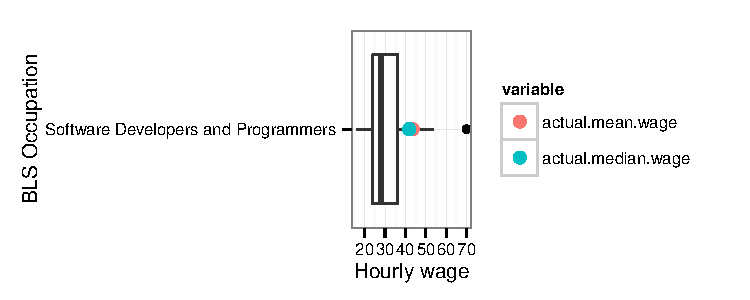
\includegraphics[width=\maxwidth]{figure/unnamed-chunk-220} 

}


\newpage\section{First-Line Supervisors of Office and Administrative Support Workers}\textbf{Occupation code:} 43-1010\newline\textbf{Typical entry education:} High school diploma or equivalent\newline\textbf{Detailed occupations:}\newline1. (43-1011)  \href{http://www.bls.gov/oes/current/oes431011.htm}{First-Line Supervisors of Office and Administrative Support Workers}\newline% latex table generated in R 3.0.2 by xtable 1.7-1 package
% Sun Nov 24 09:11:45 2013
\begin{table}[ht]
\centering
{\footnotesize
\begin{tabular}{ll|rrr}
 \textbf{Variable} & \textbf{Levels} & $\mathbf{n}$ & $\mathbf{\%}$ & $\mathbf{\sum \%}$ \\ 
  \hline
know.job &  & 2 & 6.7 & 6.7 \\ 
   & Maybe & 10 & 33.3 & 40.0 \\ 
   & No & 7 & 23.3 & 63.3 \\ 
   & Yes & 11 & 36.7 & 100.0 \\ 
   \hline
 & all & 30 & 100.0 &  \\ 
   \hline
\hline
social.knowledge & 0 & 20 & 66.7 & 66.7 \\ 
   & 1 & 4 & 13.3 & 80.0 \\ 
   & 2 & 4 & 13.3 & 93.3 \\ 
   & 3-10 & 2 & 6.7 & 100.0 \\ 
   & 10-plus & 0 & 0.0 & 100.0 \\ 
   \hline
 & all & 30 & 100.0 &  \\ 
   \hline
\hline
Answer.volume\_trend &  & 0 & 0.0 & 0.0 \\ 
   & GoDown & 5 & 16.7 & 16.7 \\ 
   & GoUp & 10 & 33.3 & 50.0 \\ 
   & StayTheSame & 15 & 50.0 & 100.0 \\ 
   \hline
 & all & 30 & 100.0 &  \\ 
   \hline
\hline
Answer.wage\_trend &  & 0 & 0.0 & 0.0 \\ 
   & GoDown & 3 & 10.0 & 10.0 \\ 
   & GoUp & 11 & 36.7 & 46.7 \\ 
   & StayTheSame & 16 & 53.3 & 100.0 \\ 
   \hline
 & all & 30 & 100.0 &  \\ 
   \hline
\hline
\end{tabular}
}
\caption{Summary statistics, nominal variables (MTurk data)} 
\label{tab1:43-1010}
\end{table}
% latex table generated in R 3.0.2 by xtable 1.7-1 package
% Sun Nov 24 09:11:45 2013
\begin{table}[ht]
\centering
{\footnotesize
\begin{tabular}{lrrrrrrrrrr}
 \textbf{Variable} & $\mathbf{n}$ & \textbf{Min} & $\mathbf{q_1}$ & $\mathbf{\widetilde{x}}$ & $\mathbf{\bar{x}}$ & $\mathbf{q_3}$ & \textbf{Max} & $\mathbf{s}$ & \textbf{IQR} & \textbf{\#NA} \\ 
  \hline
wage & 30 & 9 & 14 & 17 & 17.3 & 20 & 28 & 5.3 & 6 & 0 \\ 
  \end{tabular}
}
\caption{Summary statistics, continuous variables (MTurk data)} 
\label{tab2:43-1010}
\end{table}


{\centering 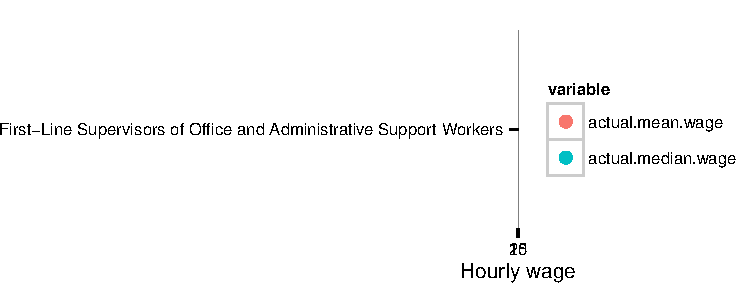
\includegraphics[width=\maxwidth]{figure/unnamed-chunk-221} 

}


\newpage\section{Miscellaneous Healthcare Support Occupations}\textbf{Occupation code:} 31-9090\newline\textbf{Typical entry education:} High school diploma or equivalent\newline\textbf{Detailed occupations:}\newline1. (31-9091)  \href{http://www.bls.gov/oes/current/oes319091.htm}{Dental Assistants}\newline2. (31-9092)  \href{http://www.bls.gov/oes/current/oes319092.htm}{Medical Assistants}\newline3. (31-9093)  \href{http://www.bls.gov/oes/current/oes319093.htm}{Medical Equipment Preparers}\newline4. (31-9094)  \href{http://www.bls.gov/oes/current/oes319094.htm}{Medical Transcriptionists}\newline5. (31-9095)  \href{http://www.bls.gov/oes/current/oes319095.htm}{Pharmacy Aides}\newline6. (31-9096)  \href{http://www.bls.gov/oes/current/oes319096.htm}{Veterinary Assistants and Laboratory Animal Caretakers}\newline7. (31-9097)  \href{http://www.bls.gov/oes/current/oes319097.htm}{Phlebotomists}\newline8. (31-9099)  \href{http://www.bls.gov/oes/current/oes319099.htm}{Healthcare Support Workers, All Other}\newline% latex table generated in R 3.0.2 by xtable 1.7-1 package
% Sun Nov 24 09:11:46 2013
\begin{table}[ht]
\centering
{\footnotesize
\begin{tabular}{ll|rrr}
 \textbf{Variable} & \textbf{Levels} & $\mathbf{n}$ & $\mathbf{\%}$ & $\mathbf{\sum \%}$ \\ 
  \hline
know.job &  & 0 & 0.0 & 0.0 \\ 
   & Maybe & 12 & 40.0 & 40.0 \\ 
   & No & 6 & 20.0 & 60.0 \\ 
   & Yes & 12 & 40.0 & 100.0 \\ 
   \hline
 & all & 30 & 100.0 &  \\ 
   \hline
\hline
social.knowledge & 0 & 18 & 62.1 & 62.1 \\ 
   & 1 & 2 & 6.9 & 69.0 \\ 
   & 2 & 4 & 13.8 & 82.8 \\ 
   & 3-10 & 4 & 13.8 & 96.5 \\ 
   & 10-plus & 1 & 3.5 & 100.0 \\ 
   \hline
 & all & 29 & 100.0 &  \\ 
   \hline
\hline
Answer.volume\_trend &  & 1 & 3.3 & 3.3 \\ 
   & GoDown & 1 & 3.3 & 6.7 \\ 
   & GoUp & 23 & 76.7 & 83.3 \\ 
   & StayTheSame & 5 & 16.7 & 100.0 \\ 
   \hline
 & all & 30 & 100.0 &  \\ 
   \hline
\hline
Answer.wage\_trend &  & 1 & 3.3 & 3.3 \\ 
   & GoDown & 1 & 3.3 & 6.7 \\ 
   & GoUp & 18 & 60.0 & 66.7 \\ 
   & StayTheSame & 10 & 33.3 & 100.0 \\ 
   \hline
 & all & 30 & 100.0 &  \\ 
   \hline
\hline
\end{tabular}
}
\caption{Summary statistics, nominal variables (MTurk data)} 
\label{tab1:31-9090}
\end{table}
% latex table generated in R 3.0.2 by xtable 1.7-1 package
% Sun Nov 24 09:11:46 2013
\begin{table}[ht]
\centering
{\footnotesize
\begin{tabular}{lrrrrrrrrrr}
 \textbf{Variable} & $\mathbf{n}$ & \textbf{Min} & $\mathbf{q_1}$ & $\mathbf{\widetilde{x}}$ & $\mathbf{\bar{x}}$ & $\mathbf{q_3}$ & \textbf{Max} & $\mathbf{s}$ & \textbf{IQR} & \textbf{\#NA} \\ 
  \hline
wage & 30 & 5 & 12.5 & 16 & 15.5 & 18 & 24 & 4.7 & 5.5 & 0 \\ 
  \end{tabular}
}
\caption{Summary statistics, continuous variables (MTurk data)} 
\label{tab2:31-9090}
\end{table}


{\centering 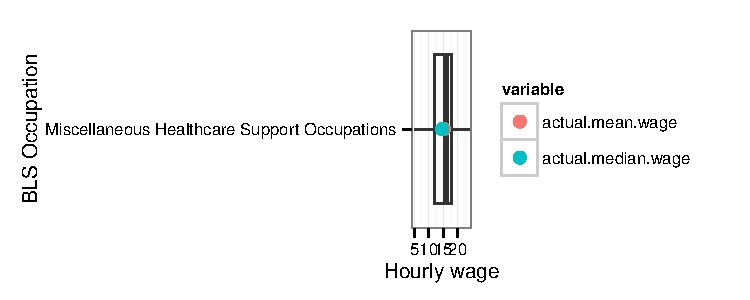
\includegraphics[width=\maxwidth]{figure/unnamed-chunk-222} 

}


\newpage\section{Miscellaneous Assemblers and Fabricators}\textbf{Occupation code:} 51-2090\newline\textbf{Typical entry education:} High school diploma or equivalent\newline\textbf{Detailed occupations:}\newline1. (51-2091)  \href{http://www.bls.gov/oes/current/oes512091.htm}{Fiberglass Laminators and Fabricators}\newline2. (51-2092)  \href{http://www.bls.gov/oes/current/oes512092.htm}{Team Assemblers}\newline3. (51-2093)  \href{http://www.bls.gov/oes/current/oes512093.htm}{Timing Device Assemblers and Adjusters}\newline4. (51-2099)  \href{http://www.bls.gov/oes/current/oes512099.htm}{Assemblers and Fabricators, All Other}\newline% latex table generated in R 3.0.2 by xtable 1.7-1 package
% Sun Nov 24 09:11:46 2013
\begin{table}[ht]
\centering
{\footnotesize
\begin{tabular}{ll|rrr}
 \textbf{Variable} & \textbf{Levels} & $\mathbf{n}$ & $\mathbf{\%}$ & $\mathbf{\sum \%}$ \\ 
  \hline
know.job &  & 0 & 0.0 & 0.0 \\ 
   & Maybe & 13 & 43.3 & 43.3 \\ 
   & No & 4 & 13.3 & 56.7 \\ 
   & Yes & 13 & 43.3 & 100.0 \\ 
   \hline
 & all & 30 & 100.0 &  \\ 
   \hline
\hline
social.knowledge & 0 & 21 & 70.0 & 70.0 \\ 
   & 1 & 3 & 10.0 & 80.0 \\ 
   & 2 & 0 & 0.0 & 80.0 \\ 
   & 3-10 & 3 & 10.0 & 90.0 \\ 
   & 10-plus & 3 & 10.0 & 100.0 \\ 
   \hline
 & all & 30 & 100.0 &  \\ 
   \hline
\hline
Answer.volume\_trend &  & 0 & 0.0 & 0.0 \\ 
   & GoDown & 17 & 56.7 & 56.7 \\ 
   & GoUp & 7 & 23.3 & 80.0 \\ 
   & StayTheSame & 6 & 20.0 & 100.0 \\ 
   \hline
 & all & 30 & 100.0 &  \\ 
   \hline
\hline
Answer.wage\_trend &  & 0 & 0.0 & 0.0 \\ 
   & GoDown & 4 & 13.3 & 13.3 \\ 
   & GoUp & 12 & 40.0 & 53.3 \\ 
   & StayTheSame & 14 & 46.7 & 100.0 \\ 
   \hline
 & all & 30 & 100.0 &  \\ 
   \hline
\hline
\end{tabular}
}
\caption{Summary statistics, nominal variables (MTurk data)} 
\label{tab1:51-2090}
\end{table}
% latex table generated in R 3.0.2 by xtable 1.7-1 package
% Sun Nov 24 09:11:46 2013
\begin{table}[ht]
\centering
{\footnotesize
\begin{tabular}{lrrrrrrrrrr}
 \textbf{Variable} & $\mathbf{n}$ & \textbf{Min} & $\mathbf{q_1}$ & $\mathbf{\widetilde{x}}$ & $\mathbf{\bar{x}}$ & $\mathbf{q_3}$ & \textbf{Max} & $\mathbf{s}$ & \textbf{IQR} & \textbf{\#NA} \\ 
  \hline
wage & 30 & 8 & 10 & 14 & 13.9 & 16 & 20 & 4.0 & 6 & 0 \\ 
  \end{tabular}
}
\caption{Summary statistics, continuous variables (MTurk data)} 
\label{tab2:51-2090}
\end{table}


{\centering 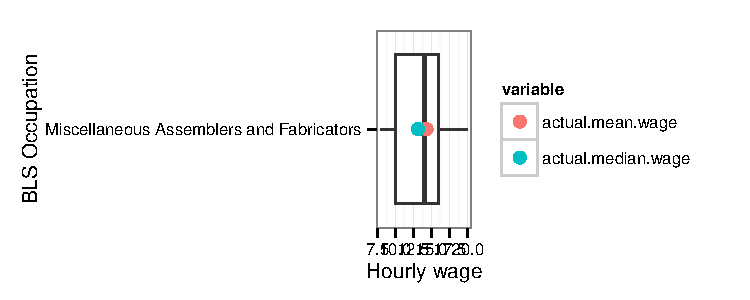
\includegraphics[width=\maxwidth]{figure/unnamed-chunk-223} 

}


\newpage\section{Maintenance and Repair Workers, General}\textbf{Occupation code:} 49-9070\newline\textbf{Typical entry education:} High school diploma or equivalent\newline\textbf{Detailed occupations:}\newline1. (49-9071)  \href{http://www.bls.gov/oes/current/oes499071.htm}{Maintenance and Repair Workers, General}\newline% latex table generated in R 3.0.2 by xtable 1.7-1 package
% Sun Nov 24 09:11:46 2013
\begin{table}[ht]
\centering
{\footnotesize
\begin{tabular}{ll|rrr}
 \textbf{Variable} & \textbf{Levels} & $\mathbf{n}$ & $\mathbf{\%}$ & $\mathbf{\sum \%}$ \\ 
  \hline
know.job &  & 0 & 0.0 & 0.0 \\ 
   & Maybe & 3 & 10.0 & 10.0 \\ 
   & No & 0 & 0.0 & 10.0 \\ 
   & Yes & 27 & 90.0 & 100.0 \\ 
   \hline
 & all & 30 & 100.0 &  \\ 
   \hline
\hline
social.knowledge & 0 & 16 & 53.3 & 53.3 \\ 
   & 1 & 6 & 20.0 & 73.3 \\ 
   & 2 & 4 & 13.3 & 86.7 \\ 
   & 3-10 & 3 & 10.0 & 96.7 \\ 
   & 10-plus & 1 & 3.3 & 100.0 \\ 
   \hline
 & all & 30 & 100.0 &  \\ 
   \hline
\hline
Answer.volume\_trend &  & 0 & 0.0 & 0.0 \\ 
   & GoDown & 1 & 3.3 & 3.3 \\ 
   & GoUp & 10 & 33.3 & 36.7 \\ 
   & StayTheSame & 19 & 63.3 & 100.0 \\ 
   \hline
 & all & 30 & 100.0 &  \\ 
   \hline
\hline
Answer.wage\_trend &  & 0 & 0.0 & 0.0 \\ 
   & GoDown & 0 & 0.0 & 0.0 \\ 
   & GoUp & 16 & 53.3 & 53.3 \\ 
   & StayTheSame & 14 & 46.7 & 100.0 \\ 
   \hline
 & all & 30 & 100.0 &  \\ 
   \hline
\hline
\end{tabular}
}
\caption{Summary statistics, nominal variables (MTurk data)} 
\label{tab1:49-9070}
\end{table}
% latex table generated in R 3.0.2 by xtable 1.7-1 package
% Sun Nov 24 09:11:46 2013
\begin{table}[ht]
\centering
{\footnotesize
\begin{tabular}{lrrrrrrrrrr}
 \textbf{Variable} & $\mathbf{n}$ & \textbf{Min} & $\mathbf{q_1}$ & $\mathbf{\widetilde{x}}$ & $\mathbf{\bar{x}}$ & $\mathbf{q_3}$ & \textbf{Max} & $\mathbf{s}$ & \textbf{IQR} & \textbf{\#NA} \\ 
  \hline
wage & 30 & 9 & 12 & 14 & 15.4 & 18 & 24 & 4.6 & 6 & 0 \\ 
  \end{tabular}
}
\caption{Summary statistics, continuous variables (MTurk data)} 
\label{tab2:49-9070}
\end{table}


{\centering 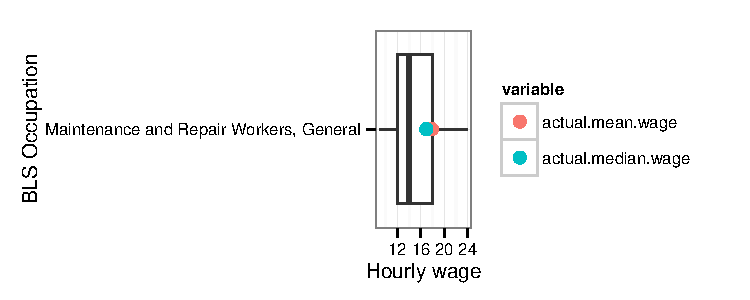
\includegraphics[width=\maxwidth]{figure/unnamed-chunk-224} 

}


\newpage\section{Teacher Assistants}\textbf{Occupation code:} 25-9040\newline\textbf{Typical entry education:} High school diploma or equivalent\newline\textbf{Detailed occupations:}\newline1. (25-9041)  \href{http://www.bls.gov/oes/current/oes259041.htm}{Teacher Assistants}\newline% latex table generated in R 3.0.2 by xtable 1.7-1 package
% Sun Nov 24 09:11:47 2013
\begin{table}[ht]
\centering
{\footnotesize
\begin{tabular}{ll|rrr}
 \textbf{Variable} & \textbf{Levels} & $\mathbf{n}$ & $\mathbf{\%}$ & $\mathbf{\sum \%}$ \\ 
  \hline
know.job &  & 0 & 0.0 & 0.0 \\ 
   & Maybe & 2 & 6.7 & 6.7 \\ 
   & No & 0 & 0.0 & 6.7 \\ 
   & Yes & 28 & 93.3 & 100.0 \\ 
   \hline
 & all & 30 & 100.0 &  \\ 
   \hline
\hline
social.knowledge & 0 & 15 & 50.0 & 50.0 \\ 
   & 1 & 10 & 33.3 & 83.3 \\ 
   & 2 & 3 & 10.0 & 93.3 \\ 
   & 3-10 & 0 & 0.0 & 93.3 \\ 
   & 10-plus & 2 & 6.7 & 100.0 \\ 
   \hline
 & all & 30 & 100.0 &  \\ 
   \hline
\hline
Answer.volume\_trend &  & 0 & 0.0 & 0.0 \\ 
   & GoDown & 11 & 36.7 & 36.7 \\ 
   & GoUp & 9 & 30.0 & 66.7 \\ 
   & StayTheSame & 10 & 33.3 & 100.0 \\ 
   \hline
 & all & 30 & 100.0 &  \\ 
   \hline
\hline
Answer.wage\_trend &  & 0 & 0.0 & 0.0 \\ 
   & GoDown & 2 & 6.7 & 6.7 \\ 
   & GoUp & 13 & 43.3 & 50.0 \\ 
   & StayTheSame & 15 & 50.0 & 100.0 \\ 
   \hline
 & all & 30 & 100.0 &  \\ 
   \hline
\hline
\end{tabular}
}
\caption{Summary statistics, nominal variables (MTurk data)} 
\label{tab1:25-9040}
\end{table}
% latex table generated in R 3.0.2 by xtable 1.7-1 package
% Sun Nov 24 09:11:47 2013
\begin{table}[ht]
\centering
{\footnotesize
\begin{tabular}{lrrrrrrrrrr}
 \textbf{Variable} & $\mathbf{n}$ & \textbf{Min} & $\mathbf{q_1}$ & $\mathbf{\widetilde{x}}$ & $\mathbf{\bar{x}}$ & $\mathbf{q_3}$ & \textbf{Max} & $\mathbf{s}$ & \textbf{IQR} & \textbf{\#NA} \\ 
  \hline
wage & 30 & 8 & 10 & 12 & 12.1 & 14 & 18 & 3.0 & 4 & 0 \\ 
  \end{tabular}
}
\caption{Summary statistics, continuous variables (MTurk data)} 
\label{tab2:25-9040}
\end{table}


{\centering 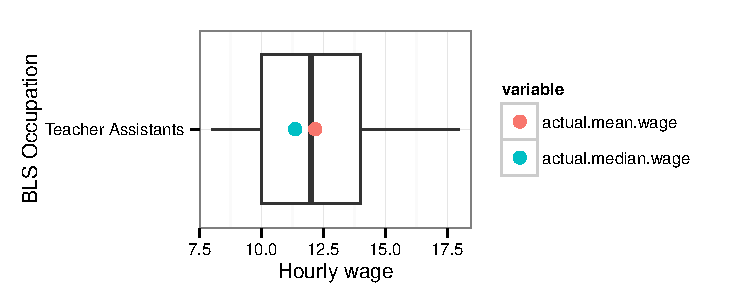
\includegraphics[width=\maxwidth]{figure/unnamed-chunk-225} 

}


\newpage\section{Accountants and Auditors}\textbf{Occupation code:} 13-2010\newline\textbf{Typical entry education:} Bachelor's degree\newline\textbf{Detailed occupations:}\newline1. (13-2011)  \href{http://www.bls.gov/oes/current/oes132011.htm}{Accountants and Auditors}\newline% latex table generated in R 3.0.2 by xtable 1.7-1 package
% Sun Nov 24 09:11:47 2013
\begin{table}[ht]
\centering
{\footnotesize
\begin{tabular}{ll|rrr}
 \textbf{Variable} & \textbf{Levels} & $\mathbf{n}$ & $\mathbf{\%}$ & $\mathbf{\sum \%}$ \\ 
  \hline
know.job &  & 1 & 3.3 & 3.3 \\ 
   & Maybe & 3 & 10.0 & 13.3 \\ 
   & No & 0 & 0.0 & 13.3 \\ 
   & Yes & 26 & 86.7 & 100.0 \\ 
   \hline
 & all & 30 & 100.0 &  \\ 
   \hline
\hline
social.knowledge & 0 & 15 & 51.7 & 51.7 \\ 
   & 1 & 9 & 31.0 & 82.8 \\ 
   & 2 & 2 & 6.9 & 89.7 \\ 
   & 3-10 & 1 & 3.5 & 93.1 \\ 
   & 10-plus & 2 & 6.9 & 100.0 \\ 
   \hline
 & all & 29 & 100.0 &  \\ 
   \hline
\hline
Answer.volume\_trend &  & 0 & 0.0 & 0.0 \\ 
   & GoDown & 3 & 10.0 & 10.0 \\ 
   & GoUp & 17 & 56.7 & 66.7 \\ 
   & StayTheSame & 10 & 33.3 & 100.0 \\ 
   \hline
 & all & 30 & 100.0 &  \\ 
   \hline
\hline
Answer.wage\_trend &  & 0 & 0.0 & 0.0 \\ 
   & GoDown & 1 & 3.3 & 3.3 \\ 
   & GoUp & 19 & 63.3 & 66.7 \\ 
   & StayTheSame & 10 & 33.3 & 100.0 \\ 
   \hline
 & all & 30 & 100.0 &  \\ 
   \hline
\hline
\end{tabular}
}
\caption{Summary statistics, nominal variables (MTurk data)} 
\label{tab1:13-2010}
\end{table}
% latex table generated in R 3.0.2 by xtable 1.7-1 package
% Sun Nov 24 09:11:47 2013
\begin{table}[ht]
\centering
{\footnotesize
\begin{tabular}{lrrrrrrrrrr}
 \textbf{Variable} & $\mathbf{n}$ & \textbf{Min} & $\mathbf{q_1}$ & $\mathbf{\widetilde{x}}$ & $\mathbf{\bar{x}}$ & $\mathbf{q_3}$ & \textbf{Max} & $\mathbf{s}$ & \textbf{IQR} & \textbf{\#NA} \\ 
  \hline
wage & 30 & 16 & 20 & 28 & 24.9 & 28 & 32 & 5.2 & 8 & 0 \\ 
  \end{tabular}
}
\caption{Summary statistics, continuous variables (MTurk data)} 
\label{tab2:13-2010}
\end{table}


{\centering 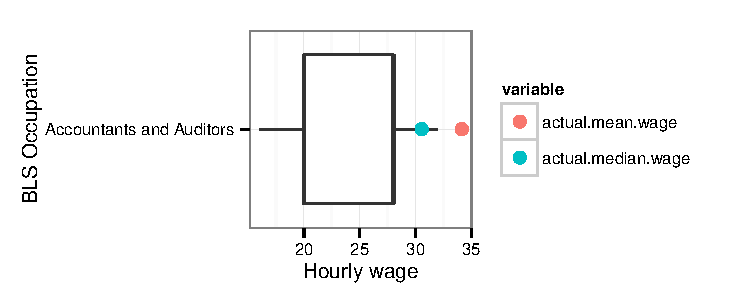
\includegraphics[width=\maxwidth]{figure/unnamed-chunk-226} 

}


\newpage\section{Security Guards and Gaming Surveillance Officers}\textbf{Occupation code:} 33-9030\newline\textbf{Typical entry education:} High school diploma or equivalent\newline\textbf{Detailed occupations:}\newline1. (33-9031)  \href{http://www.bls.gov/oes/current/oes339031.htm}{Gaming Surveillance Officers and Gaming Investigators}\newline2. (33-9032)  \href{http://www.bls.gov/oes/current/oes339032.htm}{Security Guards}\newline% latex table generated in R 3.0.2 by xtable 1.7-1 package
% Sun Nov 24 09:11:48 2013
\begin{table}[ht]
\centering
{\footnotesize
\begin{tabular}{ll|rrr}
 \textbf{Variable} & \textbf{Levels} & $\mathbf{n}$ & $\mathbf{\%}$ & $\mathbf{\sum \%}$ \\ 
  \hline
know.job &  & 0 & 0.0 & 0.0 \\ 
   & Maybe & 5 & 16.7 & 16.7 \\ 
   & No & 1 & 3.3 & 20.0 \\ 
   & Yes & 24 & 80.0 & 100.0 \\ 
   \hline
 & all & 30 & 100.0 &  \\ 
   \hline
\hline
social.knowledge & 0 & 23 & 76.7 & 76.7 \\ 
   & 1 & 5 & 16.7 & 93.3 \\ 
   & 2 & 2 & 6.7 & 100.0 \\ 
   & 3-10 & 0 & 0.0 & 100.0 \\ 
   & 10-plus & 0 & 0.0 & 100.0 \\ 
   \hline
 & all & 30 & 100.0 &  \\ 
   \hline
\hline
Answer.volume\_trend &  & 0 & 0.0 & 0.0 \\ 
   & GoDown & 3 & 10.0 & 10.0 \\ 
   & GoUp & 10 & 33.3 & 43.3 \\ 
   & StayTheSame & 17 & 56.7 & 100.0 \\ 
   \hline
 & all & 30 & 100.0 &  \\ 
   \hline
\hline
Answer.wage\_trend &  & 0 & 0.0 & 0.0 \\ 
   & GoDown & 1 & 3.3 & 3.3 \\ 
   & GoUp & 13 & 43.3 & 46.7 \\ 
   & StayTheSame & 16 & 53.3 & 100.0 \\ 
   \hline
 & all & 30 & 100.0 &  \\ 
   \hline
\hline
\end{tabular}
}
\caption{Summary statistics, nominal variables (MTurk data)} 
\label{tab1:33-9030}
\end{table}
% latex table generated in R 3.0.2 by xtable 1.7-1 package
% Sun Nov 24 09:11:48 2013
\begin{table}[ht]
\centering
{\footnotesize
\begin{tabular}{lrrrrrrrrrr}
 \textbf{Variable} & $\mathbf{n}$ & \textbf{Min} & $\mathbf{q_1}$ & $\mathbf{\widetilde{x}}$ & $\mathbf{\bar{x}}$ & $\mathbf{q_3}$ & \textbf{Max} & $\mathbf{s}$ & \textbf{IQR} & \textbf{\#NA} \\ 
  \hline
wage & 30 & 5 & 10 & 12 & 13.9 & 16 & 28 & 4.9 & 6 & 0 \\ 
  \end{tabular}
}
\caption{Summary statistics, continuous variables (MTurk data)} 
\label{tab2:33-9030}
\end{table}


{\centering 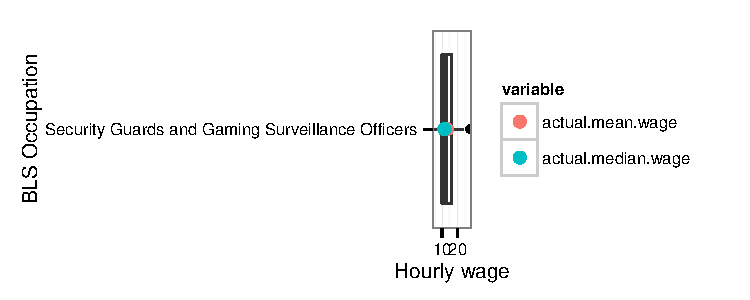
\includegraphics[width=\maxwidth]{figure/unnamed-chunk-227} 

}


\newpage\section{Secondary School Teachers}\textbf{Occupation code:} 25-2030\newline\textbf{Typical entry education:} Bachelor's degree\newline\textbf{Detailed occupations:}\newline1. (25-2031)  \href{http://www.bls.gov/oes/current/oes252031.htm}{Secondary School Teachers, Except Special and Career/Technical Education}\newline2. (25-2032)  \href{http://www.bls.gov/oes/current/oes252032.htm}{Career/Technical Education Teachers, Secondary School}\newline% latex table generated in R 3.0.2 by xtable 1.7-1 package
% Sun Nov 24 09:11:48 2013
\begin{table}[ht]
\centering
{\footnotesize
\begin{tabular}{ll|rrr}
 \textbf{Variable} & \textbf{Levels} & $\mathbf{n}$ & $\mathbf{\%}$ & $\mathbf{\sum \%}$ \\ 
  \hline
know.job &  & 1 & 3.3 & 3.3 \\ 
   & Maybe & 2 & 6.7 & 10.0 \\ 
   & No & 0 & 0.0 & 10.0 \\ 
   & Yes & 27 & 90.0 & 100.0 \\ 
   \hline
 & all & 30 & 100.0 &  \\ 
   \hline
\hline
social.knowledge & 0 & 12 & 40.0 & 40.0 \\ 
   & 1 & 3 & 10.0 & 50.0 \\ 
   & 2 & 6 & 20.0 & 70.0 \\ 
   & 3-10 & 6 & 20.0 & 90.0 \\ 
   & 10-plus & 3 & 10.0 & 100.0 \\ 
   \hline
 & all & 30 & 100.0 &  \\ 
   \hline
\hline
Answer.volume\_trend &  & 0 & 0.0 & 0.0 \\ 
   & GoDown & 4 & 13.3 & 13.3 \\ 
   & GoUp & 15 & 50.0 & 63.3 \\ 
   & StayTheSame & 11 & 36.7 & 100.0 \\ 
   \hline
 & all & 30 & 100.0 &  \\ 
   \hline
\hline
Answer.wage\_trend &  & 0 & 0.0 & 0.0 \\ 
   & GoDown & 2 & 6.7 & 6.7 \\ 
   & GoUp & 20 & 66.7 & 73.3 \\ 
   & StayTheSame & 8 & 26.7 & 100.0 \\ 
   \hline
 & all & 30 & 100.0 &  \\ 
   \hline
\hline
\end{tabular}
}
\caption{Summary statistics, nominal variables (MTurk data)} 
\label{tab1:25-2030}
\end{table}
% latex table generated in R 3.0.2 by xtable 1.7-1 package
% Sun Nov 24 09:11:48 2013
\begin{table}[ht]
\centering
{\footnotesize
\begin{tabular}{lrrrrrrrrrr}
 \textbf{Variable} & $\mathbf{n}$ & \textbf{Min} & $\mathbf{q_1}$ & $\mathbf{\widetilde{x}}$ & $\mathbf{\bar{x}}$ & $\mathbf{q_3}$ & \textbf{Max} & $\mathbf{s}$ & \textbf{IQR} & \textbf{\#NA} \\ 
  \hline
wage & 30 & 12 & 16 & 18 & 20.1 & 24 & 54 & 8.1 & 8 & 0 \\ 
  \end{tabular}
}
\caption{Summary statistics, continuous variables (MTurk data)} 
\label{tab2:25-2030}
\end{table}


{\centering 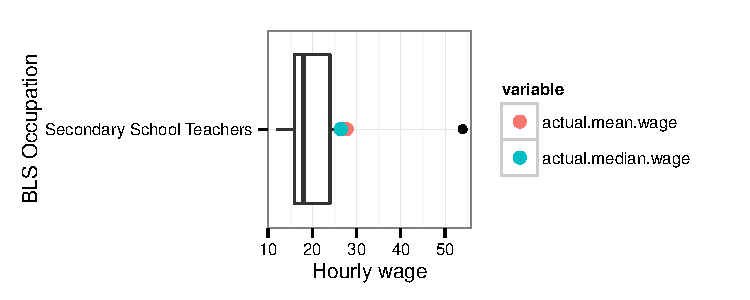
\includegraphics[width=\maxwidth]{figure/unnamed-chunk-228} 

}


\newpage\section{Personal Care Aides}\textbf{Occupation code:} 39-9020\newline\textbf{Typical entry education:} Less than high school\newline\textbf{Detailed occupations:}\newline1. (39-9021)  \href{http://www.bls.gov/oes/current/oes399021.htm}{Personal Care Aides}\newline% latex table generated in R 3.0.2 by xtable 1.7-1 package
% Sun Nov 24 09:11:49 2013
\begin{table}[ht]
\centering
{\footnotesize
\begin{tabular}{ll|rrr}
 \textbf{Variable} & \textbf{Levels} & $\mathbf{n}$ & $\mathbf{\%}$ & $\mathbf{\sum \%}$ \\ 
  \hline
know.job &  & 0 & 0.0 & 0.0 \\ 
   & Maybe & 5 & 16.7 & 16.7 \\ 
   & No & 3 & 10.0 & 26.7 \\ 
   & Yes & 22 & 73.3 & 100.0 \\ 
   \hline
 & all & 30 & 100.0 &  \\ 
   \hline
\hline
social.knowledge & 0 & 20 & 66.7 & 66.7 \\ 
   & 1 & 4 & 13.3 & 80.0 \\ 
   & 2 & 5 & 16.7 & 96.7 \\ 
   & 3-10 & 1 & 3.3 & 100.0 \\ 
   & 10-plus & 0 & 0.0 & 100.0 \\ 
   \hline
 & all & 30 & 100.0 &  \\ 
   \hline
\hline
Answer.volume\_trend &  & 0 & 0.0 & 0.0 \\ 
   & GoDown & 2 & 6.7 & 6.7 \\ 
   & GoUp & 17 & 56.7 & 63.3 \\ 
   & StayTheSame & 11 & 36.7 & 100.0 \\ 
   \hline
 & all & 30 & 100.0 &  \\ 
   \hline
\hline
Answer.wage\_trend &  & 0 & 0.0 & 0.0 \\ 
   & GoDown & 2 & 6.7 & 6.7 \\ 
   & GoUp & 16 & 53.3 & 60.0 \\ 
   & StayTheSame & 12 & 40.0 & 100.0 \\ 
   \hline
 & all & 30 & 100.0 &  \\ 
   \hline
\hline
\end{tabular}
}
\caption{Summary statistics, nominal variables (MTurk data)} 
\label{tab1:39-9020}
\end{table}
% latex table generated in R 3.0.2 by xtable 1.7-1 package
% Sun Nov 24 09:11:49 2013
\begin{table}[ht]
\centering
{\footnotesize
\begin{tabular}{lrrrrrrrrrr}
 \textbf{Variable} & $\mathbf{n}$ & \textbf{Min} & $\mathbf{q_1}$ & $\mathbf{\widetilde{x}}$ & $\mathbf{\bar{x}}$ & $\mathbf{q_3}$ & \textbf{Max} & $\mathbf{s}$ & \textbf{IQR} & \textbf{\#NA} \\ 
  \hline
wage & 30 & 9 & 12 & 14 & 14.5 & 16 & 32 & 4.6 & 4 & 0 \\ 
  \end{tabular}
}
\caption{Summary statistics, continuous variables (MTurk data)} 
\label{tab2:39-9020}
\end{table}


{\centering 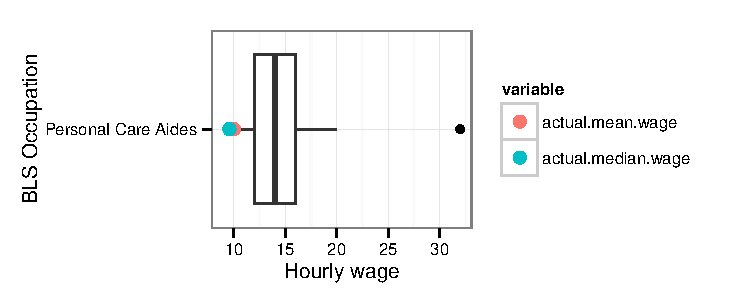
\includegraphics[width=\maxwidth]{figure/unnamed-chunk-229} 

}


\newpage\section{Receptionists and Information Clerks}\textbf{Occupation code:} 43-4170\newline\textbf{Typical entry education:} High school diploma or equivalent\newline\textbf{Detailed occupations:}\newline1. (43-4171)  \href{http://www.bls.gov/oes/current/oes434171.htm}{Receptionists and Information Clerks}\newline% latex table generated in R 3.0.2 by xtable 1.7-1 package
% Sun Nov 24 09:11:49 2013
\begin{table}[ht]
\centering
{\footnotesize
\begin{tabular}{ll|rrr}
 \textbf{Variable} & \textbf{Levels} & $\mathbf{n}$ & $\mathbf{\%}$ & $\mathbf{\sum \%}$ \\ 
  \hline
know.job &  & 0 & 0.0 & 0.0 \\ 
   & Maybe & 1 & 3.3 & 3.3 \\ 
   & No & 0 & 0.0 & 3.3 \\ 
   & Yes & 29 & 96.7 & 100.0 \\ 
   \hline
 & all & 30 & 100.0 &  \\ 
   \hline
\hline
social.knowledge & 0 & 9 & 30.0 & 30.0 \\ 
   & 1 & 7 & 23.3 & 53.3 \\ 
   & 2 & 10 & 33.3 & 86.7 \\ 
   & 3-10 & 4 & 13.3 & 100.0 \\ 
   & 10-plus & 0 & 0.0 & 100.0 \\ 
   \hline
 & all & 30 & 100.0 &  \\ 
   \hline
\hline
Answer.volume\_trend &  & 0 & 0.0 & 0.0 \\ 
   & GoDown & 7 & 23.3 & 23.3 \\ 
   & GoUp & 7 & 23.3 & 46.7 \\ 
   & StayTheSame & 16 & 53.3 & 100.0 \\ 
   \hline
 & all & 30 & 100.0 &  \\ 
   \hline
\hline
Answer.wage\_trend &  & 0 & 0.0 & 0.0 \\ 
   & GoDown & 4 & 13.3 & 13.3 \\ 
   & GoUp & 10 & 33.3 & 46.7 \\ 
   & StayTheSame & 16 & 53.3 & 100.0 \\ 
   \hline
 & all & 30 & 100.0 &  \\ 
   \hline
\hline
\end{tabular}
}
\caption{Summary statistics, nominal variables (MTurk data)} 
\label{tab1:43-4170}
\end{table}
% latex table generated in R 3.0.2 by xtable 1.7-1 package
% Sun Nov 24 09:11:49 2013
\begin{table}[ht]
\centering
{\footnotesize
\begin{tabular}{lrrrrrrrrrr}
 \textbf{Variable} & $\mathbf{n}$ & \textbf{Min} & $\mathbf{q_1}$ & $\mathbf{\widetilde{x}}$ & $\mathbf{\bar{x}}$ & $\mathbf{q_3}$ & \textbf{Max} & $\mathbf{s}$ & \textbf{IQR} & \textbf{\#NA} \\ 
  \hline
wage & 30 & 8 & 10 & 10 & 11.3 & 12 & 18 & 2.2 & 2 & 0 \\ 
  \end{tabular}
}
\caption{Summary statistics, continuous variables (MTurk data)} 
\label{tab2:43-4170}
\end{table}


{\centering 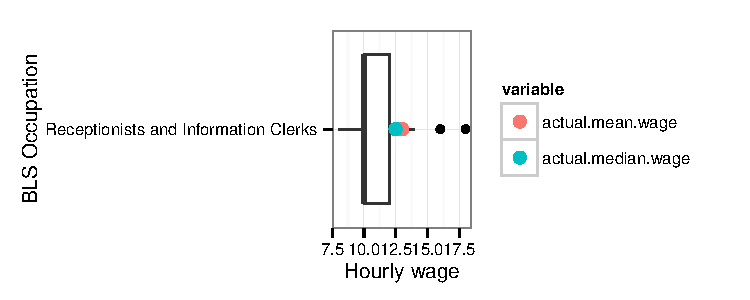
\includegraphics[width=\maxwidth]{figure/unnamed-chunk-230} 

}


\newpage\section{Miscellaneous Business Operations Specialists}\textbf{Occupation code:} 13-1190\newline\textbf{Typical entry education:} High school diploma or equivalent\newline\textbf{Detailed occupations:}\newline1. (13-1199)  \href{http://www.bls.gov/oes/current/oes131199.htm}{Business Operations Specialists, All Other}\newline% latex table generated in R 3.0.2 by xtable 1.7-1 package
% Sun Nov 24 09:11:50 2013
\begin{table}[ht]
\centering
{\footnotesize
\begin{tabular}{ll|rrr}
 \textbf{Variable} & \textbf{Levels} & $\mathbf{n}$ & $\mathbf{\%}$ & $\mathbf{\sum \%}$ \\ 
  \hline
know.job &  & 0 & 0.0 & 0.0 \\ 
   & Maybe & 10 & 33.3 & 33.3 \\ 
   & No & 20 & 66.7 & 100.0 \\ 
   & Yes & 0 & 0.0 & 100.0 \\ 
   \hline
 & all & 30 & 100.0 &  \\ 
   \hline
\hline
social.knowledge & 0 & 29 & 96.7 & 96.7 \\ 
   & 1 & 1 & 3.3 & 100.0 \\ 
   & 2 & 0 & 0.0 & 100.0 \\ 
   & 3-10 & 0 & 0.0 & 100.0 \\ 
   & 10-plus & 0 & 0.0 & 100.0 \\ 
   \hline
 & all & 30 & 100.0 &  \\ 
   \hline
\hline
Answer.volume\_trend &  & 0 & 0.0 & 0.0 \\ 
   & GoDown & 2 & 6.7 & 6.7 \\ 
   & GoUp & 6 & 20.0 & 26.7 \\ 
   & StayTheSame & 22 & 73.3 & 100.0 \\ 
   \hline
 & all & 30 & 100.0 &  \\ 
   \hline
\hline
Answer.wage\_trend &  & 0 & 0.0 & 0.0 \\ 
   & GoDown & 2 & 6.7 & 6.7 \\ 
   & GoUp & 11 & 36.7 & 43.3 \\ 
   & StayTheSame & 17 & 56.7 & 100.0 \\ 
   \hline
 & all & 30 & 100.0 &  \\ 
   \hline
\hline
\end{tabular}
}
\caption{Summary statistics, nominal variables (MTurk data)} 
\label{tab1:13-1190}
\end{table}
% latex table generated in R 3.0.2 by xtable 1.7-1 package
% Sun Nov 24 09:11:50 2013
\begin{table}[ht]
\centering
{\footnotesize
\begin{tabular}{lrrrrrrrrrr}
 \textbf{Variable} & $\mathbf{n}$ & \textbf{Min} & $\mathbf{q_1}$ & $\mathbf{\widetilde{x}}$ & $\mathbf{\bar{x}}$ & $\mathbf{q_3}$ & \textbf{Max} & $\mathbf{s}$ & \textbf{IQR} & \textbf{\#NA} \\ 
  \hline
wage & 30 & 10 & 16 & 20 & 20.5 & 24 & 54 & 8.1 & 8 & 0 \\ 
  \end{tabular}
}
\caption{Summary statistics, continuous variables (MTurk data)} 
\label{tab2:13-1190}
\end{table}


{\centering 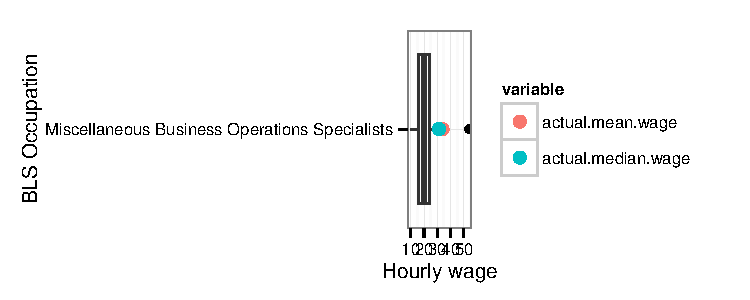
\includegraphics[width=\maxwidth]{figure/unnamed-chunk-231} 

}


\newpage\section{Supervisors of Food Preparation and Serving Workers}\textbf{Occupation code:} 35-1010\newline\textbf{Typical entry education:} High school diploma or equivalent\newline\textbf{Detailed occupations:}\newline1. (35-1011)  \href{http://www.bls.gov/oes/current/oes351011.htm}{Chefs and Head Cooks}\newline2. (35-1012)  \href{http://www.bls.gov/oes/current/oes351012.htm}{First-Line Supervisors of Food Preparation and Serving Workers}\newline% latex table generated in R 3.0.2 by xtable 1.7-1 package
% Sun Nov 24 09:11:50 2013
\begin{table}[ht]
\centering
{\footnotesize
\begin{tabular}{ll|rrr}
 \textbf{Variable} & \textbf{Levels} & $\mathbf{n}$ & $\mathbf{\%}$ & $\mathbf{\sum \%}$ \\ 
  \hline
know.job &  & 0 & 0.0 & 0.0 \\ 
   & Maybe & 3 & 10.0 & 10.0 \\ 
   & No & 0 & 0.0 & 10.0 \\ 
   & Yes & 27 & 90.0 & 100.0 \\ 
   \hline
 & all & 30 & 100.0 &  \\ 
   \hline
\hline
social.knowledge & 0 & 17 & 56.7 & 56.7 \\ 
   & 1 & 4 & 13.3 & 70.0 \\ 
   & 2 & 5 & 16.7 & 86.7 \\ 
   & 3-10 & 3 & 10.0 & 96.7 \\ 
   & 10-plus & 1 & 3.3 & 100.0 \\ 
   \hline
 & all & 30 & 100.0 &  \\ 
   \hline
\hline
Answer.volume\_trend &  & 0 & 0.0 & 0.0 \\ 
   & GoDown & 1 & 3.3 & 3.3 \\ 
   & GoUp & 10 & 33.3 & 36.7 \\ 
   & StayTheSame & 19 & 63.3 & 100.0 \\ 
   \hline
 & all & 30 & 100.0 &  \\ 
   \hline
\hline
Answer.wage\_trend &  & 0 & 0.0 & 0.0 \\ 
   & GoDown & 0 & 0.0 & 0.0 \\ 
   & GoUp & 12 & 40.0 & 40.0 \\ 
   & StayTheSame & 18 & 60.0 & 100.0 \\ 
   \hline
 & all & 30 & 100.0 &  \\ 
   \hline
\hline
\end{tabular}
}
\caption{Summary statistics, nominal variables (MTurk data)} 
\label{tab1:35-1010}
\end{table}
% latex table generated in R 3.0.2 by xtable 1.7-1 package
% Sun Nov 24 09:11:50 2013
\begin{table}[ht]
\centering
{\footnotesize
\begin{tabular}{lrrrrrrrrrr}
 \textbf{Variable} & $\mathbf{n}$ & \textbf{Min} & $\mathbf{q_1}$ & $\mathbf{\widetilde{x}}$ & $\mathbf{\bar{x}}$ & $\mathbf{q_3}$ & \textbf{Max} & $\mathbf{s}$ & \textbf{IQR} & \textbf{\#NA} \\ 
  \hline
wage & 30 & 5 & 10 & 12 & 12.9 & 14 & 24 & 3.8 & 4 & 0 \\ 
  \end{tabular}
}
\caption{Summary statistics, continuous variables (MTurk data)} 
\label{tab2:35-1010}
\end{table}


{\centering 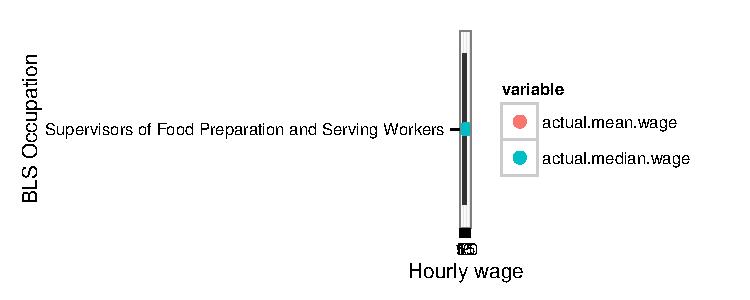
\includegraphics[width=\maxwidth]{figure/unnamed-chunk-232} 

}


\newpage\section{Grounds Maintenance Workers}\textbf{Occupation code:} 37-3010\newline\textbf{Typical entry education:} Less than high school\newline\textbf{Detailed occupations:}\newline1. (37-3011)  \href{http://www.bls.gov/oes/current/oes373011.htm}{Landscaping and Groundskeeping Workers}\newline2. (37-3012)  \href{http://www.bls.gov/oes/current/oes373012.htm}{Pesticide Handlers, Sprayers, and Applicators, Vegetation}\newline3. (37-3013)  \href{http://www.bls.gov/oes/current/oes373013.htm}{Tree Trimmers and Pruners}\newline4. (37-3019)  \href{http://www.bls.gov/oes/current/oes373019.htm}{Grounds Maintenance Workers, All Other}\newline% latex table generated in R 3.0.2 by xtable 1.7-1 package
% Sun Nov 24 09:11:51 2013
\begin{table}[ht]
\centering
{\footnotesize
\begin{tabular}{ll|rrr}
 \textbf{Variable} & \textbf{Levels} & $\mathbf{n}$ & $\mathbf{\%}$ & $\mathbf{\sum \%}$ \\ 
  \hline
know.job &  & 0 & 0.0 & 0.0 \\ 
   & Maybe & 1 & 3.3 & 3.3 \\ 
   & No & 0 & 0.0 & 3.3 \\ 
   & Yes & 29 & 96.7 & 100.0 \\ 
   \hline
 & all & 30 & 100.0 &  \\ 
   \hline
\hline
social.knowledge & 0 & 10 & 34.5 & 34.5 \\ 
   & 1 & 12 & 41.4 & 75.9 \\ 
   & 2 & 2 & 6.9 & 82.8 \\ 
   & 3-10 & 5 & 17.2 & 100.0 \\ 
   & 10-plus & 0 & 0.0 & 100.0 \\ 
   \hline
 & all & 29 & 100.0 &  \\ 
   \hline
\hline
Answer.volume\_trend &  & 0 & 0.0 & 0.0 \\ 
   & GoDown & 2 & 6.7 & 6.7 \\ 
   & GoUp & 8 & 26.7 & 33.3 \\ 
   & StayTheSame & 20 & 66.7 & 100.0 \\ 
   \hline
 & all & 30 & 100.0 &  \\ 
   \hline
\hline
Answer.wage\_trend &  & 0 & 0.0 & 0.0 \\ 
   & GoDown & 3 & 10.0 & 10.0 \\ 
   & GoUp & 16 & 53.3 & 63.3 \\ 
   & StayTheSame & 11 & 36.7 & 100.0 \\ 
   \hline
 & all & 30 & 100.0 &  \\ 
   \hline
\hline
\end{tabular}
}
\caption{Summary statistics, nominal variables (MTurk data)} 
\label{tab1:37-3010}
\end{table}
% latex table generated in R 3.0.2 by xtable 1.7-1 package
% Sun Nov 24 09:11:51 2013
\begin{table}[ht]
\centering
{\footnotesize
\begin{tabular}{lrrrrrrrrrr}
 \textbf{Variable} & $\mathbf{n}$ & \textbf{Min} & $\mathbf{q_1}$ & $\mathbf{\widetilde{x}}$ & $\mathbf{\bar{x}}$ & $\mathbf{q_3}$ & \textbf{Max} & $\mathbf{s}$ & \textbf{IQR} & \textbf{\#NA} \\ 
  \hline
wage & 30 & 8 & 10 & 10 & 11.8 & 14 & 20 & 3.4 & 4 & 0 \\ 
  \end{tabular}
}
\caption{Summary statistics, continuous variables (MTurk data)} 
\label{tab2:37-3010}
\end{table}


{\centering 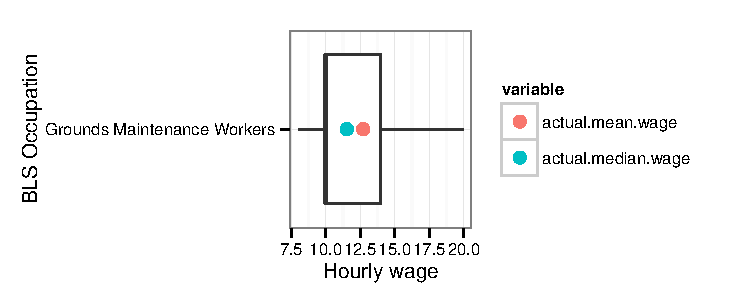
\includegraphics[width=\maxwidth]{figure/unnamed-chunk-233} 

}


\newpage\section{Miscellaneous Teachers and Instructors}\textbf{Occupation code:} 25-3090\newline\textbf{Typical entry education:} Bachelor's degree\newline\textbf{Detailed occupations:}\newline1. (25-3098)  \href{http://www.bls.gov/oes/current/oes253098.htm}{Substitute Teachers}\newline2. (25-3099)  \href{http://www.bls.gov/oes/current/oes253099.htm}{Teachers and Instructors, All Other, Except Substitute Teachers}\newline% latex table generated in R 3.0.2 by xtable 1.7-1 package
% Sun Nov 24 09:11:51 2013
\begin{table}[ht]
\centering
{\footnotesize
\begin{tabular}{ll|rrr}
 \textbf{Variable} & \textbf{Levels} & $\mathbf{n}$ & $\mathbf{\%}$ & $\mathbf{\sum \%}$ \\ 
  \hline
know.job &  & 0 & 0.0 & 0.0 \\ 
   & Maybe & 4 & 13.3 & 13.3 \\ 
   & No & 1 & 3.3 & 16.7 \\ 
   & Yes & 25 & 83.3 & 100.0 \\ 
   \hline
 & all & 30 & 100.0 &  \\ 
   \hline
\hline
social.knowledge & 0 & 8 & 26.7 & 26.7 \\ 
   & 1 & 9 & 30.0 & 56.7 \\ 
   & 2 & 2 & 6.7 & 63.3 \\ 
   & 3-10 & 10 & 33.3 & 96.7 \\ 
   & 10-plus & 1 & 3.3 & 100.0 \\ 
   \hline
 & all & 30 & 100.0 &  \\ 
   \hline
\hline
Answer.volume\_trend &  & 0 & 0.0 & 0.0 \\ 
   & GoDown & 7 & 23.3 & 23.3 \\ 
   & GoUp & 18 & 60.0 & 83.3 \\ 
   & StayTheSame & 5 & 16.7 & 100.0 \\ 
   \hline
 & all & 30 & 100.0 &  \\ 
   \hline
\hline
Answer.wage\_trend &  & 0 & 0.0 & 0.0 \\ 
   & GoDown & 5 & 16.7 & 16.7 \\ 
   & GoUp & 20 & 66.7 & 83.3 \\ 
   & StayTheSame & 5 & 16.7 & 100.0 \\ 
   \hline
 & all & 30 & 100.0 &  \\ 
   \hline
\hline
\end{tabular}
}
\caption{Summary statistics, nominal variables (MTurk data)} 
\label{tab1:25-3090}
\end{table}
% latex table generated in R 3.0.2 by xtable 1.7-1 package
% Sun Nov 24 09:11:51 2013
\begin{table}[ht]
\centering
{\footnotesize
\begin{tabular}{lrrrrrrrrrr}
 \textbf{Variable} & $\mathbf{n}$ & \textbf{Min} & $\mathbf{q_1}$ & $\mathbf{\widetilde{x}}$ & $\mathbf{\bar{x}}$ & $\mathbf{q_3}$ & \textbf{Max} & $\mathbf{s}$ & \textbf{IQR} & \textbf{\#NA} \\ 
  \hline
wage & 30 & 10 & 14 & 18 & 17.5 & 20 & 28 & 4.6 & 6 & 0 \\ 
  \end{tabular}
}
\caption{Summary statistics, continuous variables (MTurk data)} 
\label{tab2:25-3090}
\end{table}


{\centering 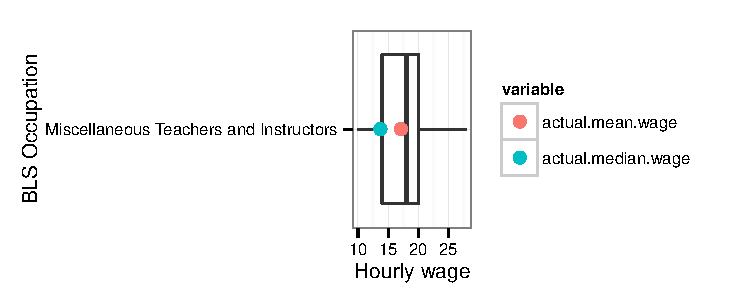
\includegraphics[width=\maxwidth]{figure/unnamed-chunk-234} 

}


\newpage\section{Miscellaneous Production Workers}\textbf{Occupation code:} 51-9190\newline\textbf{Typical entry education:} Less than high school\newline\textbf{Detailed occupations:}\newline1. (51-9191)  \href{http://www.bls.gov/oes/current/oes519191.htm}{Adhesive Bonding Machine Operators and Tenders}\newline2. (51-9192)  \href{http://www.bls.gov/oes/current/oes519192.htm}{Cleaning, Washing, and Metal Pickling Equipment Operators and Tenders}\newline3. (51-9193)  \href{http://www.bls.gov/oes/current/oes519193.htm}{Cooling and Freezing Equipment Operators and Tenders}\newline4. (51-9194)  \href{http://www.bls.gov/oes/current/oes519194.htm}{Etchers and Engravers}\newline5. (51-9195)  \href{http://www.bls.gov/oes/current/oes519195.htm}{Molders, Shapers, and Casters, Except Metal and Plastic}\newline6. (51-9196)  \href{http://www.bls.gov/oes/current/oes519196.htm}{Paper Goods Machine Setters, Operators, and Tenders}\newline7. (51-9197)  \href{http://www.bls.gov/oes/current/oes519197.htm}{Tire Builders}\newline8. (51-9198)  \href{http://www.bls.gov/oes/current/oes519198.htm}{Helpers--Production Workers}\newline9. (51-9199)  \href{http://www.bls.gov/oes/current/oes519199.htm}{Production Workers, All Other}\newline% latex table generated in R 3.0.2 by xtable 1.7-1 package
% Sun Nov 24 09:11:52 2013
\begin{table}[ht]
\centering
{\footnotesize
\begin{tabular}{ll|rrr}
 \textbf{Variable} & \textbf{Levels} & $\mathbf{n}$ & $\mathbf{\%}$ & $\mathbf{\sum \%}$ \\ 
  \hline
know.job &  & 0 & 0.0 & 0.0 \\ 
   & Maybe & 15 & 50.0 & 50.0 \\ 
   & No & 4 & 13.3 & 63.3 \\ 
   & Yes & 11 & 36.7 & 100.0 \\ 
   \hline
 & all & 30 & 100.0 &  \\ 
   \hline
\hline
social.knowledge & 0 & 18 & 60.0 & 60.0 \\ 
   & 1 & 5 & 16.7 & 76.7 \\ 
   & 2 & 4 & 13.3 & 90.0 \\ 
   & 3-10 & 3 & 10.0 & 100.0 \\ 
   & 10-plus & 0 & 0.0 & 100.0 \\ 
   \hline
 & all & 30 & 100.0 &  \\ 
   \hline
\hline
Answer.volume\_trend &  & 0 & 0.0 & 0.0 \\ 
   & GoDown & 15 & 50.0 & 50.0 \\ 
   & GoUp & 8 & 26.7 & 76.7 \\ 
   & StayTheSame & 7 & 23.3 & 100.0 \\ 
   \hline
 & all & 30 & 100.0 &  \\ 
   \hline
\hline
Answer.wage\_trend &  & 0 & 0.0 & 0.0 \\ 
   & GoDown & 5 & 16.7 & 16.7 \\ 
   & GoUp & 10 & 33.3 & 50.0 \\ 
   & StayTheSame & 15 & 50.0 & 100.0 \\ 
   \hline
 & all & 30 & 100.0 &  \\ 
   \hline
\hline
\end{tabular}
}
\caption{Summary statistics, nominal variables (MTurk data)} 
\label{tab1:51-9190}
\end{table}
% latex table generated in R 3.0.2 by xtable 1.7-1 package
% Sun Nov 24 09:11:52 2013
\begin{table}[ht]
\centering
{\footnotesize
\begin{tabular}{lrrrrrrrrrr}
 \textbf{Variable} & $\mathbf{n}$ & \textbf{Min} & $\mathbf{q_1}$ & $\mathbf{\widetilde{x}}$ & $\mathbf{\bar{x}}$ & $\mathbf{q_3}$ & \textbf{Max} & $\mathbf{s}$ & \textbf{IQR} & \textbf{\#NA} \\ 
  \hline
wage & 30 & 5 & 9 & 10 & 10.6 & 11.5 & 28 & 4.3 & 2.5 & 0 \\ 
  \end{tabular}
}
\caption{Summary statistics, continuous variables (MTurk data)} 
\label{tab2:51-9190}
\end{table}


{\centering 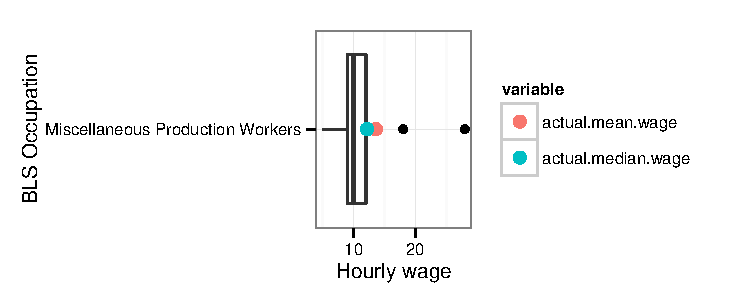
\includegraphics[width=\maxwidth]{figure/unnamed-chunk-235} 

}


\newpage\section{Construction Laborers}\textbf{Occupation code:} 47-2060\newline\textbf{Typical entry education:} Less than high school\newline\textbf{Detailed occupations:}\newline1. (47-2061)  \href{http://www.bls.gov/oes/current/oes472061.htm}{Construction Laborers}\newline% latex table generated in R 3.0.2 by xtable 1.7-1 package
% Sun Nov 24 09:11:52 2013
\begin{table}[ht]
\centering
{\footnotesize
\begin{tabular}{ll|rrr}
 \textbf{Variable} & \textbf{Levels} & $\mathbf{n}$ & $\mathbf{\%}$ & $\mathbf{\sum \%}$ \\ 
  \hline
know.job &  & 0 & 0.0 & 0.0 \\ 
   & Maybe & 1 & 3.3 & 3.3 \\ 
   & No & 0 & 0.0 & 3.3 \\ 
   & Yes & 29 & 96.7 & 100.0 \\ 
   \hline
 & all & 30 & 100.0 &  \\ 
   \hline
\hline
social.knowledge & 0 & 11 & 36.7 & 36.7 \\ 
   & 1 & 8 & 26.7 & 63.3 \\ 
   & 2 & 3 & 10.0 & 73.3 \\ 
   & 3-10 & 7 & 23.3 & 96.7 \\ 
   & 10-plus & 1 & 3.3 & 100.0 \\ 
   \hline
 & all & 30 & 100.0 &  \\ 
   \hline
\hline
Answer.volume\_trend &  & 0 & 0.0 & 0.0 \\ 
   & GoDown & 2 & 6.7 & 6.7 \\ 
   & GoUp & 15 & 50.0 & 56.7 \\ 
   & StayTheSame & 13 & 43.3 & 100.0 \\ 
   \hline
 & all & 30 & 100.0 &  \\ 
   \hline
\hline
Answer.wage\_trend &  & 0 & 0.0 & 0.0 \\ 
   & GoDown & 4 & 13.3 & 13.3 \\ 
   & GoUp & 16 & 53.3 & 66.7 \\ 
   & StayTheSame & 10 & 33.3 & 100.0 \\ 
   \hline
 & all & 30 & 100.0 &  \\ 
   \hline
\hline
\end{tabular}
}
\caption{Summary statistics, nominal variables (MTurk data)} 
\label{tab1:47-2060}
\end{table}
% latex table generated in R 3.0.2 by xtable 1.7-1 package
% Sun Nov 24 09:11:52 2013
\begin{table}[ht]
\centering
{\footnotesize
\begin{tabular}{lrrrrrrrrrr}
 \textbf{Variable} & $\mathbf{n}$ & \textbf{Min} & $\mathbf{q_1}$ & $\mathbf{\widetilde{x}}$ & $\mathbf{\bar{x}}$ & $\mathbf{q_3}$ & \textbf{Max} & $\mathbf{s}$ & \textbf{IQR} & \textbf{\#NA} \\ 
  \hline
wage & 30 & 9 & 12 & 16 & 17.6 & 20 & 36 & 7.2 & 8 & 0 \\ 
  \end{tabular}
}
\caption{Summary statistics, continuous variables (MTurk data)} 
\label{tab2:47-2060}
\end{table}


{\centering 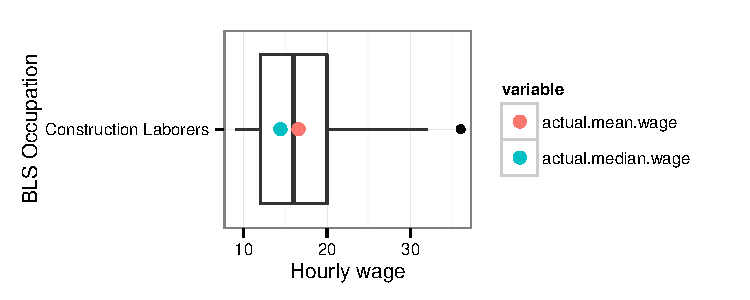
\includegraphics[width=\maxwidth]{figure/unnamed-chunk-236} 

}


\newpage\section{Food Preparation Workers}\textbf{Occupation code:} 35-2020\newline\textbf{Typical entry education:} Less than high school\newline\textbf{Detailed occupations:}\newline1. (35-2021)  \href{http://www.bls.gov/oes/current/oes352021.htm}{Food Preparation Workers}\newline% latex table generated in R 3.0.2 by xtable 1.7-1 package
% Sun Nov 24 09:11:52 2013
\begin{table}[ht]
\centering
{\footnotesize
\begin{tabular}{ll|rrr}
 \textbf{Variable} & \textbf{Levels} & $\mathbf{n}$ & $\mathbf{\%}$ & $\mathbf{\sum \%}$ \\ 
  \hline
know.job &  & 0 & 0.0 & 0.0 \\ 
   & Maybe & 2 & 6.7 & 6.7 \\ 
   & No & 0 & 0.0 & 6.7 \\ 
   & Yes & 28 & 93.3 & 100.0 \\ 
   \hline
 & all & 30 & 100.0 &  \\ 
   \hline
\hline
social.knowledge & 0 & 17 & 56.7 & 56.7 \\ 
   & 1 & 3 & 10.0 & 66.7 \\ 
   & 2 & 5 & 16.7 & 83.3 \\ 
   & 3-10 & 2 & 6.7 & 90.0 \\ 
   & 10-plus & 3 & 10.0 & 100.0 \\ 
   \hline
 & all & 30 & 100.0 &  \\ 
   \hline
\hline
Answer.volume\_trend &  & 0 & 0.0 & 0.0 \\ 
   & GoDown & 1 & 3.3 & 3.3 \\ 
   & GoUp & 15 & 50.0 & 53.3 \\ 
   & StayTheSame & 14 & 46.7 & 100.0 \\ 
   \hline
 & all & 30 & 100.0 &  \\ 
   \hline
\hline
Answer.wage\_trend &  & 0 & 0.0 & 0.0 \\ 
   & GoDown & 1 & 3.3 & 3.3 \\ 
   & GoUp & 13 & 43.3 & 46.7 \\ 
   & StayTheSame & 16 & 53.3 & 100.0 \\ 
   \hline
 & all & 30 & 100.0 &  \\ 
   \hline
\hline
\end{tabular}
}
\caption{Summary statistics, nominal variables (MTurk data)} 
\label{tab1:35-2020}
\end{table}
% latex table generated in R 3.0.2 by xtable 1.7-1 package
% Sun Nov 24 09:11:52 2013
\begin{table}[ht]
\centering
{\footnotesize
\begin{tabular}{lrrrrrrrrrr}
 \textbf{Variable} & $\mathbf{n}$ & \textbf{Min} & $\mathbf{q_1}$ & $\mathbf{\widetilde{x}}$ & $\mathbf{\bar{x}}$ & $\mathbf{q_3}$ & \textbf{Max} & $\mathbf{s}$ & \textbf{IQR} & \textbf{\#NA} \\ 
  \hline
wage & 30 & 5 & 8 & 9 & 9.2 & 10 & 18 & 2.9 & 2 & 0 \\ 
  \end{tabular}
}
\caption{Summary statistics, continuous variables (MTurk data)} 
\label{tab2:35-2020}
\end{table}


{\centering 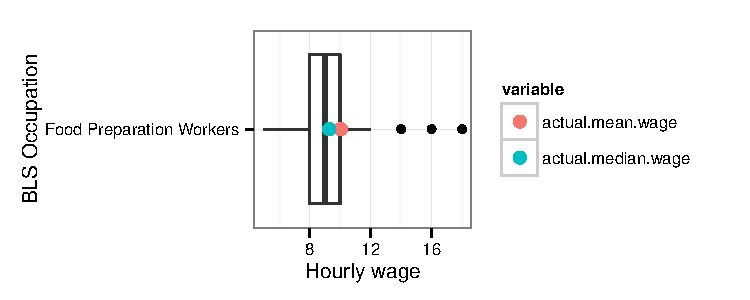
\includegraphics[width=\maxwidth]{figure/unnamed-chunk-237} 

}


\newpage\section{Automotive Technicians and Repairers}\textbf{Occupation code:} 49-3020\newline\textbf{Typical entry education:} High school diploma or equivalent\newline\textbf{Detailed occupations:}\newline1. (49-3021)  \href{http://www.bls.gov/oes/current/oes493021.htm}{Automotive Body and Related Repairers}\newline2. (49-3022)  \href{http://www.bls.gov/oes/current/oes493022.htm}{Automotive Glass Installers and Repairers}\newline3. (49-3023)  \href{http://www.bls.gov/oes/current/oes493023.htm}{Automotive Service Technicians and Mechanics}\newline% latex table generated in R 3.0.2 by xtable 1.7-1 package
% Sun Nov 24 09:11:53 2013
\begin{table}[ht]
\centering
{\footnotesize
\begin{tabular}{ll|rrr}
 \textbf{Variable} & \textbf{Levels} & $\mathbf{n}$ & $\mathbf{\%}$ & $\mathbf{\sum \%}$ \\ 
  \hline
know.job &  & 0 & 0.0 & 0.0 \\ 
   & Maybe & 1 & 3.3 & 3.3 \\ 
   & No & 0 & 0.0 & 3.3 \\ 
   & Yes & 29 & 96.7 & 100.0 \\ 
   \hline
 & all & 30 & 100.0 &  \\ 
   \hline
\hline
social.knowledge & 0 & 11 & 36.7 & 36.7 \\ 
   & 1 & 11 & 36.7 & 73.3 \\ 
   & 2 & 4 & 13.3 & 86.7 \\ 
   & 3-10 & 4 & 13.3 & 100.0 \\ 
   & 10-plus & 0 & 0.0 & 100.0 \\ 
   \hline
 & all & 30 & 100.0 &  \\ 
   \hline
\hline
Answer.volume\_trend &  & 0 & 0.0 & 0.0 \\ 
   & GoDown & 6 & 20.0 & 20.0 \\ 
   & GoUp & 11 & 36.7 & 56.7 \\ 
   & StayTheSame & 13 & 43.3 & 100.0 \\ 
   \hline
 & all & 30 & 100.0 &  \\ 
   \hline
\hline
Answer.wage\_trend &  & 0 & 0.0 & 0.0 \\ 
   & GoDown & 3 & 10.0 & 10.0 \\ 
   & GoUp & 18 & 60.0 & 70.0 \\ 
   & StayTheSame & 9 & 30.0 & 100.0 \\ 
   \hline
 & all & 30 & 100.0 &  \\ 
   \hline
\hline
\end{tabular}
}
\caption{Summary statistics, nominal variables (MTurk data)} 
\label{tab1:49-3020}
\end{table}
% latex table generated in R 3.0.2 by xtable 1.7-1 package
% Sun Nov 24 09:11:53 2013
\begin{table}[ht]
\centering
{\footnotesize
\begin{tabular}{lrrrrrrrrrr}
 \textbf{Variable} & $\mathbf{n}$ & \textbf{Min} & $\mathbf{q_1}$ & $\mathbf{\widetilde{x}}$ & $\mathbf{\bar{x}}$ & $\mathbf{q_3}$ & \textbf{Max} & $\mathbf{s}$ & \textbf{IQR} & \textbf{\#NA} \\ 
  \hline
wage & 30 & 5 & 14 & 16 & 19.7 & 24 & 70 & 11.7 & 10 & 0 \\ 
  \end{tabular}
}
\caption{Summary statistics, continuous variables (MTurk data)} 
\label{tab2:49-3020}
\end{table}


{\centering 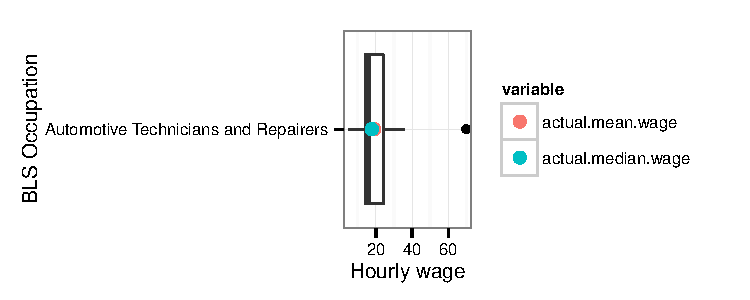
\includegraphics[width=\maxwidth]{figure/unnamed-chunk-238} 

}


\newpage\section{Licensed Practical and Licensed Vocational Nurses}\textbf{Occupation code:} 29-2060\newline\textbf{Typical entry education:} Postsecondary non-degree award\newline\textbf{Detailed occupations:}\newline1. (29-2061)  \href{http://www.bls.gov/oes/current/oes292061.htm}{Licensed Practical and Licensed Vocational Nurses}\newline% latex table generated in R 3.0.2 by xtable 1.7-1 package
% Sun Nov 24 09:11:53 2013
\begin{table}[ht]
\centering
{\footnotesize
\begin{tabular}{ll|rrr}
 \textbf{Variable} & \textbf{Levels} & $\mathbf{n}$ & $\mathbf{\%}$ & $\mathbf{\sum \%}$ \\ 
  \hline
know.job &  & 0 & 0.0 & 0.0 \\ 
   & Maybe & 7 & 24.1 & 24.1 \\ 
   & No & 0 & 0.0 & 24.1 \\ 
   & Yes & 22 & 75.9 & 100.0 \\ 
   \hline
 & all & 29 & 100.0 &  \\ 
   \hline
\hline
social.knowledge & 0 & 11 & 37.9 & 37.9 \\ 
   & 1 & 8 & 27.6 & 65.5 \\ 
   & 2 & 5 & 17.2 & 82.8 \\ 
   & 3-10 & 3 & 10.3 & 93.1 \\ 
   & 10-plus & 2 & 6.9 & 100.0 \\ 
   \hline
 & all & 29 & 100.0 &  \\ 
   \hline
\hline
Answer.volume\_trend &  & 0 & 0.0 & 0.0 \\ 
   & GoDown & 1 & 3.5 & 3.5 \\ 
   & GoUp & 22 & 75.9 & 79.3 \\ 
   & StayTheSame & 6 & 20.7 & 100.0 \\ 
   \hline
 & all & 29 & 100.0 &  \\ 
   \hline
\hline
Answer.wage\_trend &  & 0 & 0.0 & 0.0 \\ 
   & GoDown & 2 & 6.9 & 6.9 \\ 
   & GoUp & 21 & 72.4 & 79.3 \\ 
   & StayTheSame & 6 & 20.7 & 100.0 \\ 
   \hline
 & all & 29 & 100.0 &  \\ 
   \hline
\hline
\end{tabular}
}
\caption{Summary statistics, nominal variables (MTurk data)} 
\label{tab1:29-2060}
\end{table}
% latex table generated in R 3.0.2 by xtable 1.7-1 package
% Sun Nov 24 09:11:53 2013
\begin{table}[ht]
\centering
{\footnotesize
\begin{tabular}{lrrrrrrrrrr}
 \textbf{Variable} & $\mathbf{n}$ & \textbf{Min} & $\mathbf{q_1}$ & $\mathbf{\widetilde{x}}$ & $\mathbf{\bar{x}}$ & $\mathbf{q_3}$ & \textbf{Max} & $\mathbf{s}$ & \textbf{IQR} & \textbf{\#NA} \\ 
  \hline
wage & 29 & 10 & 20 & 24 & 24.4 & 28 & 50 & 7.4 & 8 & 0 \\ 
  \end{tabular}
}
\caption{Summary statistics, continuous variables (MTurk data)} 
\label{tab2:29-2060}
\end{table}


{\centering 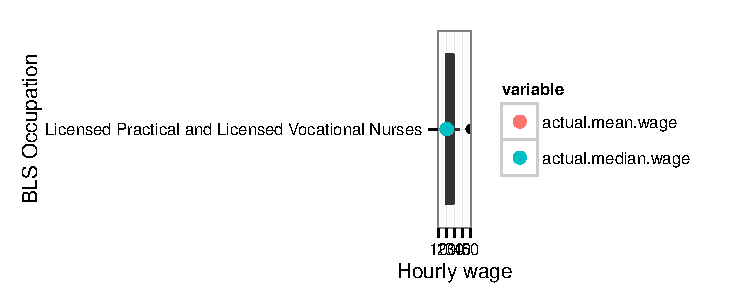
\includegraphics[width=\maxwidth]{figure/unnamed-chunk-239} 

}


\newpage\section{Computer Support Specialists}\textbf{Occupation code:} 15-1150\newline\textbf{Typical entry education:} Some college, no degree\newline\textbf{Detailed occupations:}\newline1. (15-1151)  \href{http://www.bls.gov/oes/current/oes151151.htm}{Computer User Support Specialists}\newline2. (15-1152)  \href{http://www.bls.gov/oes/current/oes151152.htm}{Computer Network Support Specialists}\newline% latex table generated in R 3.0.2 by xtable 1.7-1 package
% Sun Nov 24 09:11:54 2013
\begin{table}[ht]
\centering
{\footnotesize
\begin{tabular}{ll|rrr}
 \textbf{Variable} & \textbf{Levels} & $\mathbf{n}$ & $\mathbf{\%}$ & $\mathbf{\sum \%}$ \\ 
  \hline
know.job &  & 0 & 0.0 & 0.0 \\ 
   & Maybe & 5 & 16.7 & 16.7 \\ 
   & No & 0 & 0.0 & 16.7 \\ 
   & Yes & 25 & 83.3 & 100.0 \\ 
   \hline
 & all & 30 & 100.0 &  \\ 
   \hline
\hline
social.knowledge & 0 & 12 & 40.0 & 40.0 \\ 
   & 1 & 10 & 33.3 & 73.3 \\ 
   & 2 & 2 & 6.7 & 80.0 \\ 
   & 3-10 & 5 & 16.7 & 96.7 \\ 
   & 10-plus & 1 & 3.3 & 100.0 \\ 
   \hline
 & all & 30 & 100.0 &  \\ 
   \hline
\hline
Answer.volume\_trend &  & 0 & 0.0 & 0.0 \\ 
   & GoDown & 1 & 3.3 & 3.3 \\ 
   & GoUp & 28 & 93.3 & 96.7 \\ 
   & StayTheSame & 1 & 3.3 & 100.0 \\ 
   \hline
 & all & 30 & 100.0 &  \\ 
   \hline
\hline
Answer.wage\_trend &  & 0 & 0.0 & 0.0 \\ 
   & GoDown & 5 & 16.7 & 16.7 \\ 
   & GoUp & 23 & 76.7 & 93.3 \\ 
   & StayTheSame & 2 & 6.7 & 100.0 \\ 
   \hline
 & all & 30 & 100.0 &  \\ 
   \hline
\hline
\end{tabular}
}
\caption{Summary statistics, nominal variables (MTurk data)} 
\label{tab1:15-1150}
\end{table}
% latex table generated in R 3.0.2 by xtable 1.7-1 package
% Sun Nov 24 09:11:54 2013
\begin{table}[ht]
\centering
{\footnotesize
\begin{tabular}{lrrrrrrrrrr}
 \textbf{Variable} & $\mathbf{n}$ & \textbf{Min} & $\mathbf{q_1}$ & $\mathbf{\widetilde{x}}$ & $\mathbf{\bar{x}}$ & $\mathbf{q_3}$ & \textbf{Max} & $\mathbf{s}$ & \textbf{IQR} & \textbf{\#NA} \\ 
  \hline
wage & 30 & 12 & 14.5 & 19 & 18.6 & 20 & 28 & 4.8 & 5.5 & 0 \\ 
  \end{tabular}
}
\caption{Summary statistics, continuous variables (MTurk data)} 
\label{tab2:15-1150}
\end{table}


{\centering 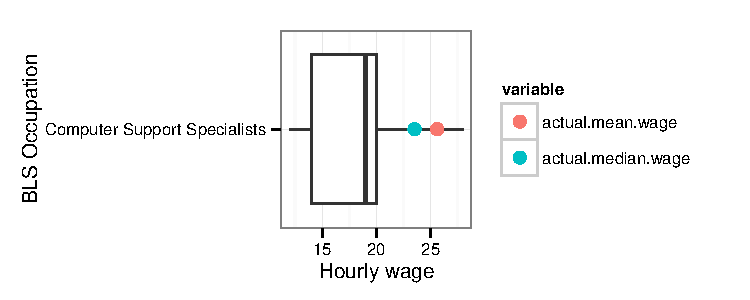
\includegraphics[width=\maxwidth]{figure/unnamed-chunk-240} 

}


\newpage\section{Shipping, Receiving, and Traffic Clerks}\textbf{Occupation code:} 43-5070\newline\textbf{Typical entry education:} High school diploma or equivalent\newline\textbf{Detailed occupations:}\newline1. (43-5071)  \href{http://www.bls.gov/oes/current/oes435071.htm}{Shipping, Receiving, and Traffic Clerks}\newline% latex table generated in R 3.0.2 by xtable 1.7-1 package
% Sun Nov 24 09:11:54 2013
\begin{table}[ht]
\centering
{\footnotesize
\begin{tabular}{ll|rrr}
 \textbf{Variable} & \textbf{Levels} & $\mathbf{n}$ & $\mathbf{\%}$ & $\mathbf{\sum \%}$ \\ 
  \hline
know.job &  & 1 & 3.3 & 3.3 \\ 
   & Maybe & 8 & 26.7 & 30.0 \\ 
   & No & 2 & 6.7 & 36.7 \\ 
   & Yes & 19 & 63.3 & 100.0 \\ 
   \hline
 & all & 30 & 100.0 &  \\ 
   \hline
\hline
social.knowledge & 0 & 21 & 70.0 & 70.0 \\ 
   & 1 & 5 & 16.7 & 86.7 \\ 
   & 2 & 1 & 3.3 & 90.0 \\ 
   & 3-10 & 3 & 10.0 & 100.0 \\ 
   & 10-plus & 0 & 0.0 & 100.0 \\ 
   \hline
 & all & 30 & 100.0 &  \\ 
   \hline
\hline
Answer.volume\_trend &  & 0 & 0.0 & 0.0 \\ 
   & GoDown & 7 & 23.3 & 23.3 \\ 
   & GoUp & 10 & 33.3 & 56.7 \\ 
   & StayTheSame & 13 & 43.3 & 100.0 \\ 
   \hline
 & all & 30 & 100.0 &  \\ 
   \hline
\hline
Answer.wage\_trend &  & 0 & 0.0 & 0.0 \\ 
   & GoDown & 2 & 6.7 & 6.7 \\ 
   & GoUp & 10 & 33.3 & 40.0 \\ 
   & StayTheSame & 18 & 60.0 & 100.0 \\ 
   \hline
 & all & 30 & 100.0 &  \\ 
   \hline
\hline
\end{tabular}
}
\caption{Summary statistics, nominal variables (MTurk data)} 
\label{tab1:43-5070}
\end{table}
% latex table generated in R 3.0.2 by xtable 1.7-1 package
% Sun Nov 24 09:11:54 2013
\begin{table}[ht]
\centering
{\footnotesize
\begin{tabular}{lrrrrrrrrrr}
 \textbf{Variable} & $\mathbf{n}$ & \textbf{Min} & $\mathbf{q_1}$ & $\mathbf{\widetilde{x}}$ & $\mathbf{\bar{x}}$ & $\mathbf{q_3}$ & \textbf{Max} & $\mathbf{s}$ & \textbf{IQR} & \textbf{\#NA} \\ 
  \hline
wage & 30 & 9 & 12 & 12 & 13.1 & 15.5 & 20 & 2.9 & 3.5 & 0 \\ 
  \end{tabular}
}
\caption{Summary statistics, continuous variables (MTurk data)} 
\label{tab2:43-5070}
\end{table}


{\centering 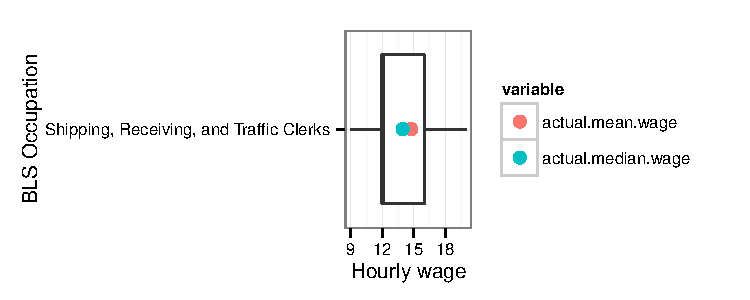
\includegraphics[width=\maxwidth]{figure/unnamed-chunk-241} 

}


\newpage\section{Miscellaneous Sales Representatives, Services}\textbf{Occupation code:} 41-3090\newline\textbf{Typical entry education:} High school diploma or equivalent\newline\textbf{Detailed occupations:}\newline1. (41-3099)  \href{http://www.bls.gov/oes/current/oes413099.htm}{Sales Representatives, Services, All Other}\newline% latex table generated in R 3.0.2 by xtable 1.7-1 package
% Sun Nov 24 09:11:55 2013
\begin{table}[ht]
\centering
{\footnotesize
\begin{tabular}{ll|rrr}
 \textbf{Variable} & \textbf{Levels} & $\mathbf{n}$ & $\mathbf{\%}$ & $\mathbf{\sum \%}$ \\ 
  \hline
know.job &  & 0 & 0.0 & 0.0 \\ 
   & Maybe & 10 & 33.3 & 33.3 \\ 
   & No & 0 & 0.0 & 33.3 \\ 
   & Yes & 20 & 66.7 & 100.0 \\ 
   \hline
 & all & 30 & 100.0 &  \\ 
   \hline
\hline
social.knowledge & 0 & 16 & 53.3 & 53.3 \\ 
   & 1 & 4 & 13.3 & 66.7 \\ 
   & 2 & 5 & 16.7 & 83.3 \\ 
   & 3-10 & 4 & 13.3 & 96.7 \\ 
   & 10-plus & 1 & 3.3 & 100.0 \\ 
   \hline
 & all & 30 & 100.0 &  \\ 
   \hline
\hline
Answer.volume\_trend &  & 0 & 0.0 & 0.0 \\ 
   & GoDown & 4 & 13.3 & 13.3 \\ 
   & GoUp & 10 & 33.3 & 46.7 \\ 
   & StayTheSame & 16 & 53.3 & 100.0 \\ 
   \hline
 & all & 30 & 100.0 &  \\ 
   \hline
\hline
Answer.wage\_trend &  & 0 & 0.0 & 0.0 \\ 
   & GoDown & 4 & 13.3 & 13.3 \\ 
   & GoUp & 7 & 23.3 & 36.7 \\ 
   & StayTheSame & 19 & 63.3 & 100.0 \\ 
   \hline
 & all & 30 & 100.0 &  \\ 
   \hline
\hline
\end{tabular}
}
\caption{Summary statistics, nominal variables (MTurk data)} 
\label{tab1:41-3090}
\end{table}
% latex table generated in R 3.0.2 by xtable 1.7-1 package
% Sun Nov 24 09:11:55 2013
\begin{table}[ht]
\centering
{\footnotesize
\begin{tabular}{lrrrrrrrrrr}
 \textbf{Variable} & $\mathbf{n}$ & \textbf{Min} & $\mathbf{q_1}$ & $\mathbf{\widetilde{x}}$ & $\mathbf{\bar{x}}$ & $\mathbf{q_3}$ & \textbf{Max} & $\mathbf{s}$ & \textbf{IQR} & \textbf{\#NA} \\ 
  \hline
wage & 30 & 5 & 10.5 & 14 & 14.2 & 16 & 28 & 5.0 & 5.5 & 0 \\ 
  \end{tabular}
}
\caption{Summary statistics, continuous variables (MTurk data)} 
\label{tab2:41-3090}
\end{table}


{\centering 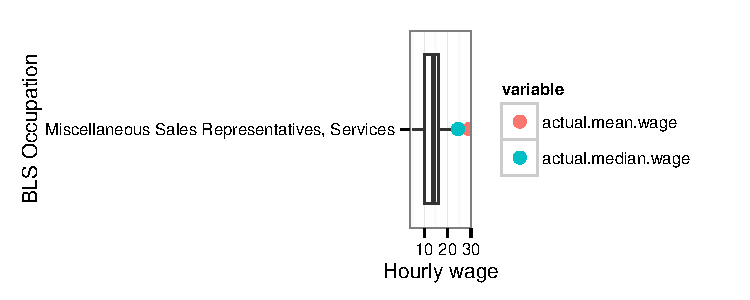
\includegraphics[width=\maxwidth]{figure/unnamed-chunk-242} 

}


\newpage\section{Health Practitioner Support Technologists and Technicians}\textbf{Occupation code:} 29-2050\newline\textbf{Typical entry education:} High school diploma or equivalent\newline\textbf{Detailed occupations:}\newline1. (29-2051)  \href{http://www.bls.gov/oes/current/oes292051.htm}{Dietetic Technicians}\newline2. (29-2052)  \href{http://www.bls.gov/oes/current/oes292052.htm}{Pharmacy Technicians}\newline3. (29-2053)  \href{http://www.bls.gov/oes/current/oes292053.htm}{Psychiatric Technicians}\newline4. (29-2054)  \href{http://www.bls.gov/oes/current/oes292054.htm}{Respiratory Therapy Technicians}\newline5. (29-2055)  \href{http://www.bls.gov/oes/current/oes292055.htm}{Surgical Technologists}\newline6. (29-2056)  \href{http://www.bls.gov/oes/current/oes292056.htm}{Veterinary Technologists and Technicians}\newline7. (29-2057)  \href{http://www.bls.gov/oes/current/oes292057.htm}{Ophthalmic Medical Technicians}\newline% latex table generated in R 3.0.2 by xtable 1.7-1 package
% Sun Nov 24 09:11:55 2013
\begin{table}[ht]
\centering
{\footnotesize
\begin{tabular}{ll|rrr}
 \textbf{Variable} & \textbf{Levels} & $\mathbf{n}$ & $\mathbf{\%}$ & $\mathbf{\sum \%}$ \\ 
  \hline
know.job &  & 0 & 0.0 & 0.0 \\ 
   & Maybe & 11 & 36.7 & 36.7 \\ 
   & No & 2 & 6.7 & 43.3 \\ 
   & Yes & 17 & 56.7 & 100.0 \\ 
   \hline
 & all & 30 & 100.0 &  \\ 
   \hline
\hline
social.knowledge & 0 & 20 & 66.7 & 66.7 \\ 
   & 1 & 7 & 23.3 & 90.0 \\ 
   & 2 & 1 & 3.3 & 93.3 \\ 
   & 3-10 & 1 & 3.3 & 96.7 \\ 
   & 10-plus & 1 & 3.3 & 100.0 \\ 
   \hline
 & all & 30 & 100.0 &  \\ 
   \hline
\hline
Answer.volume\_trend &  & 0 & 0.0 & 0.0 \\ 
   & GoDown & 4 & 13.3 & 13.3 \\ 
   & GoUp & 19 & 63.3 & 76.7 \\ 
   & StayTheSame & 7 & 23.3 & 100.0 \\ 
   \hline
 & all & 30 & 100.0 &  \\ 
   \hline
\hline
Answer.wage\_trend &  & 0 & 0.0 & 0.0 \\ 
   & GoDown & 4 & 13.3 & 13.3 \\ 
   & GoUp & 21 & 70.0 & 83.3 \\ 
   & StayTheSame & 5 & 16.7 & 100.0 \\ 
   \hline
 & all & 30 & 100.0 &  \\ 
   \hline
\hline
\end{tabular}
}
\caption{Summary statistics, nominal variables (MTurk data)} 
\label{tab1:29-2050}
\end{table}
% latex table generated in R 3.0.2 by xtable 1.7-1 package
% Sun Nov 24 09:11:55 2013
\begin{table}[ht]
\centering
{\footnotesize
\begin{tabular}{lrrrrrrrrrr}
 \textbf{Variable} & $\mathbf{n}$ & \textbf{Min} & $\mathbf{q_1}$ & $\mathbf{\widetilde{x}}$ & $\mathbf{\bar{x}}$ & $\mathbf{q_3}$ & \textbf{Max} & $\mathbf{s}$ & \textbf{IQR} & \textbf{\#NA} \\ 
  \hline
wage & 30 & 12 & 16 & 20 & 21.8 & 27 & 50 & 8.5 & 11 & 0 \\ 
  \end{tabular}
}
\caption{Summary statistics, continuous variables (MTurk data)} 
\label{tab2:29-2050}
\end{table}


{\centering 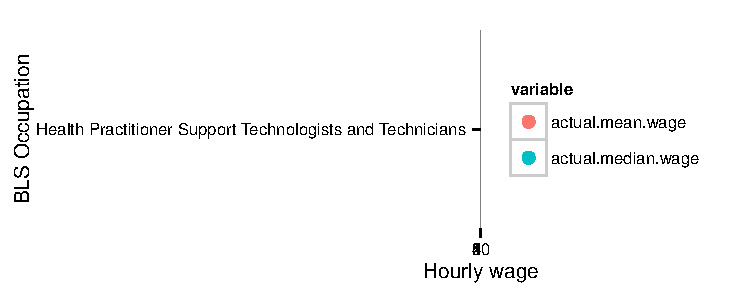
\includegraphics[width=\maxwidth]{figure/unnamed-chunk-243} 

}


\newpage\section{Bus Drivers}\textbf{Occupation code:} 53-3020\newline\textbf{Typical entry education:} High school diploma or equivalent\newline\textbf{Detailed occupations:}\newline1. (53-3021)  \href{http://www.bls.gov/oes/current/oes533021.htm}{Bus Drivers, Transit and Intercity}\newline2. (53-3022)  \href{http://www.bls.gov/oes/current/oes533022.htm}{Bus Drivers, School or Special Client}\newline% latex table generated in R 3.0.2 by xtable 1.7-1 package
% Sun Nov 24 09:11:56 2013
\begin{table}[ht]
\centering
{\footnotesize
\begin{tabular}{ll|rrr}
 \textbf{Variable} & \textbf{Levels} & $\mathbf{n}$ & $\mathbf{\%}$ & $\mathbf{\sum \%}$ \\ 
  \hline
know.job &  & 0 & 0.0 & 0.0 \\ 
   & Maybe & 0 & 0.0 & 0.0 \\ 
   & No & 0 & 0.0 & 0.0 \\ 
   & Yes & 30 & 100.0 & 100.0 \\ 
   \hline
 & all & 30 & 100.0 &  \\ 
   \hline
\hline
social.knowledge & 0 & 19 & 63.3 & 63.3 \\ 
   & 1 & 7 & 23.3 & 86.7 \\ 
   & 2 & 3 & 10.0 & 96.7 \\ 
   & 3-10 & 1 & 3.3 & 100.0 \\ 
   & 10-plus & 0 & 0.0 & 100.0 \\ 
   \hline
 & all & 30 & 100.0 &  \\ 
   \hline
\hline
Answer.volume\_trend &  & 0 & 0.0 & 0.0 \\ 
   & GoDown & 9 & 30.0 & 30.0 \\ 
   & GoUp & 8 & 26.7 & 56.7 \\ 
   & StayTheSame & 13 & 43.3 & 100.0 \\ 
   \hline
 & all & 30 & 100.0 &  \\ 
   \hline
\hline
Answer.wage\_trend &  & 0 & 0.0 & 0.0 \\ 
   & GoDown & 3 & 10.0 & 10.0 \\ 
   & GoUp & 13 & 43.3 & 53.3 \\ 
   & StayTheSame & 14 & 46.7 & 100.0 \\ 
   \hline
 & all & 30 & 100.0 &  \\ 
   \hline
\hline
\end{tabular}
}
\caption{Summary statistics, nominal variables (MTurk data)} 
\label{tab1:53-3020}
\end{table}
% latex table generated in R 3.0.2 by xtable 1.7-1 package
% Sun Nov 24 09:11:56 2013
\begin{table}[ht]
\centering
{\footnotesize
\begin{tabular}{lrrrrrrrrrr}
 \textbf{Variable} & $\mathbf{n}$ & \textbf{Min} & $\mathbf{q_1}$ & $\mathbf{\widetilde{x}}$ & $\mathbf{\bar{x}}$ & $\mathbf{q_3}$ & \textbf{Max} & $\mathbf{s}$ & \textbf{IQR} & \textbf{\#NA} \\ 
  \hline
wage & 30 & 8 & 10 & 13 & 14.2 & 16 & 32 & 5.1 & 6 & 0 \\ 
  \end{tabular}
}
\caption{Summary statistics, continuous variables (MTurk data)} 
\label{tab2:53-3020}
\end{table}


{\centering 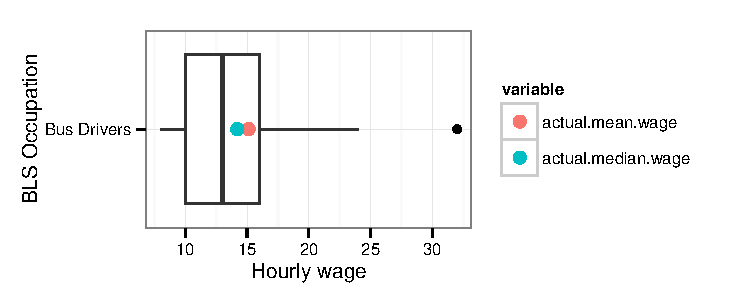
\includegraphics[width=\maxwidth]{figure/unnamed-chunk-244} 

}


\newpage\section{Counter and Rental Clerks and Parts Salespersons}\textbf{Occupation code:} 41-2020\newline\textbf{Typical entry education:} Less than high school\newline\textbf{Detailed occupations:}\newline1. (41-2021)  \href{http://www.bls.gov/oes/current/oes412021.htm}{Counter and Rental Clerks}\newline2. (41-2022)  \href{http://www.bls.gov/oes/current/oes412022.htm}{Parts Salespersons}\newline% latex table generated in R 3.0.2 by xtable 1.7-1 package
% Sun Nov 24 09:11:56 2013
\begin{table}[ht]
\centering
{\footnotesize
\begin{tabular}{ll|rrr}
 \textbf{Variable} & \textbf{Levels} & $\mathbf{n}$ & $\mathbf{\%}$ & $\mathbf{\sum \%}$ \\ 
  \hline
know.job &  & 0 & 0.0 & 0.0 \\ 
   & Maybe & 8 & 26.7 & 26.7 \\ 
   & No & 2 & 6.7 & 33.3 \\ 
   & Yes & 20 & 66.7 & 100.0 \\ 
   \hline
 & all & 30 & 100.0 &  \\ 
   \hline
\hline
social.knowledge & 0 & 16 & 53.3 & 53.3 \\ 
   & 1 & 9 & 30.0 & 83.3 \\ 
   & 2 & 3 & 10.0 & 93.3 \\ 
   & 3-10 & 2 & 6.7 & 100.0 \\ 
   & 10-plus & 0 & 0.0 & 100.0 \\ 
   \hline
 & all & 30 & 100.0 &  \\ 
   \hline
\hline
Answer.volume\_trend &  & 0 & 0.0 & 0.0 \\ 
   & GoDown & 6 & 20.0 & 20.0 \\ 
   & GoUp & 7 & 23.3 & 43.3 \\ 
   & StayTheSame & 17 & 56.7 & 100.0 \\ 
   \hline
 & all & 30 & 100.0 &  \\ 
   \hline
\hline
Answer.wage\_trend &  & 0 & 0.0 & 0.0 \\ 
   & GoDown & 5 & 16.7 & 16.7 \\ 
   & GoUp & 12 & 40.0 & 56.7 \\ 
   & StayTheSame & 13 & 43.3 & 100.0 \\ 
   \hline
 & all & 30 & 100.0 &  \\ 
   \hline
\hline
\end{tabular}
}
\caption{Summary statistics, nominal variables (MTurk data)} 
\label{tab1:41-2020}
\end{table}
% latex table generated in R 3.0.2 by xtable 1.7-1 package
% Sun Nov 24 09:11:56 2013
\begin{table}[ht]
\centering
{\footnotesize
\begin{tabular}{lrrrrrrrrrr}
 \textbf{Variable} & $\mathbf{n}$ & \textbf{Min} & $\mathbf{q_1}$ & $\mathbf{\widetilde{x}}$ & $\mathbf{\bar{x}}$ & $\mathbf{q_3}$ & \textbf{Max} & $\mathbf{s}$ & \textbf{IQR} & \textbf{\#NA} \\ 
  \hline
wage & 30 & 5 & 9 & 10 & 10.4 & 12 & 18 & 3.0 & 3 & 0 \\ 
  \end{tabular}
}
\caption{Summary statistics, continuous variables (MTurk data)} 
\label{tab2:41-2020}
\end{table}


{\centering 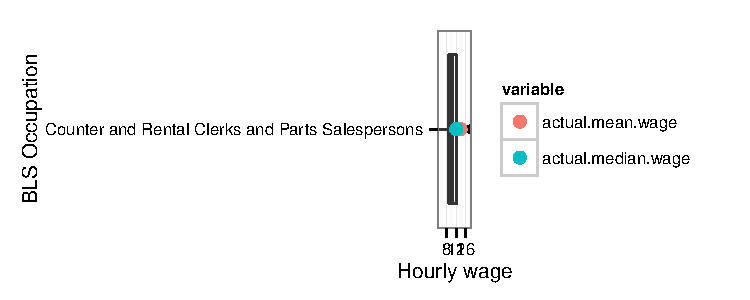
\includegraphics[width=\maxwidth]{figure/unnamed-chunk-245} 

}


\newpage\section{Police Officers}\textbf{Occupation code:} 33-3050\newline\textbf{Typical entry education:} High school diploma or equivalent\newline\textbf{Detailed occupations:}\newline1. (33-3051)  \href{http://www.bls.gov/oes/current/oes333051.htm}{Police and Sheriff's Patrol Officers}\newline2. (33-3052)  \href{http://www.bls.gov/oes/current/oes333052.htm}{Transit and Railroad Police}\newline% latex table generated in R 3.0.2 by xtable 1.7-1 package
% Sun Nov 24 09:11:57 2013
\begin{table}[ht]
\centering
{\footnotesize
\begin{tabular}{ll|rrr}
 \textbf{Variable} & \textbf{Levels} & $\mathbf{n}$ & $\mathbf{\%}$ & $\mathbf{\sum \%}$ \\ 
  \hline
know.job &  & 1 & 3.3 & 3.3 \\ 
   & Maybe & 0 & 0.0 & 3.3 \\ 
   & No & 0 & 0.0 & 3.3 \\ 
   & Yes & 29 & 96.7 & 100.0 \\ 
   \hline
 & all & 30 & 100.0 &  \\ 
   \hline
\hline
social.knowledge & 0 & 7 & 23.3 & 23.3 \\ 
   & 1 & 10 & 33.3 & 56.7 \\ 
   & 2 & 5 & 16.7 & 73.3 \\ 
   & 3-10 & 6 & 20.0 & 93.3 \\ 
   & 10-plus & 2 & 6.7 & 100.0 \\ 
   \hline
 & all & 30 & 100.0 &  \\ 
   \hline
\hline
Answer.volume\_trend &  & 0 & 0.0 & 0.0 \\ 
   & GoDown & 3 & 10.0 & 10.0 \\ 
   & GoUp & 19 & 63.3 & 73.3 \\ 
   & StayTheSame & 8 & 26.7 & 100.0 \\ 
   \hline
 & all & 30 & 100.0 &  \\ 
   \hline
\hline
Answer.wage\_trend &  & 0 & 0.0 & 0.0 \\ 
   & GoDown & 2 & 6.7 & 6.7 \\ 
   & GoUp & 18 & 60.0 & 66.7 \\ 
   & StayTheSame & 10 & 33.3 & 100.0 \\ 
   \hline
 & all & 30 & 100.0 &  \\ 
   \hline
\hline
\end{tabular}
}
\caption{Summary statistics, nominal variables (MTurk data)} 
\label{tab1:33-3050}
\end{table}
% latex table generated in R 3.0.2 by xtable 1.7-1 package
% Sun Nov 24 09:11:57 2013
\begin{table}[ht]
\centering
{\footnotesize
\begin{tabular}{lrrrrrrrrrr}
 \textbf{Variable} & $\mathbf{n}$ & \textbf{Min} & $\mathbf{q_1}$ & $\mathbf{\widetilde{x}}$ & $\mathbf{\bar{x}}$ & $\mathbf{q_3}$ & \textbf{Max} & $\mathbf{s}$ & \textbf{IQR} & \textbf{\#NA} \\ 
  \hline
wage & 30 & 12 & 18 & 20 & 24.9 & 31 & 50 & 9.9 & 13 & 0 \\ 
  \end{tabular}
}
\caption{Summary statistics, continuous variables (MTurk data)} 
\label{tab2:33-3050}
\end{table}


{\centering 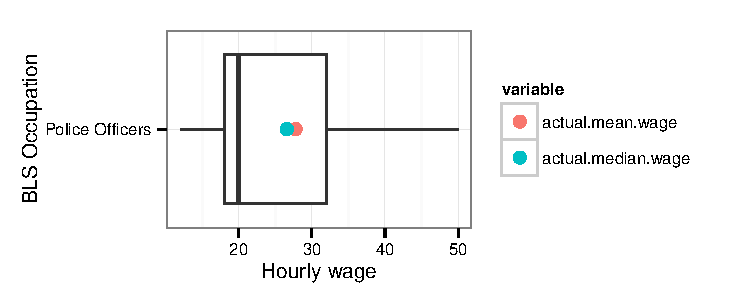
\includegraphics[width=\maxwidth]{figure/unnamed-chunk-246} 

}


\newpage\section{Miscellaneous Community and Social Service Specialists}\textbf{Occupation code:} 21-1090\newline\textbf{Typical entry education:} High school diploma or equivalent\newline\textbf{Detailed occupations:}\newline1. (21-1091)  \href{http://www.bls.gov/oes/current/oes211091.htm}{Health Educators}\newline2. (21-1092)  \href{http://www.bls.gov/oes/current/oes211092.htm}{Probation Officers and Correctional Treatment Specialists}\newline3. (21-1093)  \href{http://www.bls.gov/oes/current/oes211093.htm}{Social and Human Service Assistants}\newline4. (21-1094)  \href{http://www.bls.gov/oes/current/oes211094.htm}{Community Health Workers}\newline5. (21-1099)  \href{http://www.bls.gov/oes/current/oes211099.htm}{Community and Social Service Specialists, All Other}\newline% latex table generated in R 3.0.2 by xtable 1.7-1 package
% Sun Nov 24 09:11:57 2013
\begin{table}[ht]
\centering
{\footnotesize
\begin{tabular}{ll|rrr}
 \textbf{Variable} & \textbf{Levels} & $\mathbf{n}$ & $\mathbf{\%}$ & $\mathbf{\sum \%}$ \\ 
  \hline
know.job &  & 0 & 0.0 & 0.0 \\ 
   & Maybe & 15 & 50.0 & 50.0 \\ 
   & No & 8 & 26.7 & 76.7 \\ 
   & Yes & 7 & 23.3 & 100.0 \\ 
   \hline
 & all & 30 & 100.0 &  \\ 
   \hline
\hline
social.knowledge & 0 & 23 & 76.7 & 76.7 \\ 
   & 1 & 5 & 16.7 & 93.3 \\ 
   & 2 & 1 & 3.3 & 96.7 \\ 
   & 3-10 & 1 & 3.3 & 100.0 \\ 
   & 10-plus & 0 & 0.0 & 100.0 \\ 
   \hline
 & all & 30 & 100.0 &  \\ 
   \hline
\hline
Answer.volume\_trend &  & 0 & 0.0 & 0.0 \\ 
   & GoDown & 6 & 20.0 & 20.0 \\ 
   & GoUp & 15 & 50.0 & 70.0 \\ 
   & StayTheSame & 9 & 30.0 & 100.0 \\ 
   \hline
 & all & 30 & 100.0 &  \\ 
   \hline
\hline
Answer.wage\_trend &  & 0 & 0.0 & 0.0 \\ 
   & GoDown & 2 & 6.7 & 6.7 \\ 
   & GoUp & 15 & 50.0 & 56.7 \\ 
   & StayTheSame & 13 & 43.3 & 100.0 \\ 
   \hline
 & all & 30 & 100.0 &  \\ 
   \hline
\hline
\end{tabular}
}
\caption{Summary statistics, nominal variables (MTurk data)} 
\label{tab1:21-1090}
\end{table}
% latex table generated in R 3.0.2 by xtable 1.7-1 package
% Sun Nov 24 09:11:57 2013
\begin{table}[ht]
\centering
{\footnotesize
\begin{tabular}{lrrrrrrrrrr}
 \textbf{Variable} & $\mathbf{n}$ & \textbf{Min} & $\mathbf{q_1}$ & $\mathbf{\widetilde{x}}$ & $\mathbf{\bar{x}}$ & $\mathbf{q_3}$ & \textbf{Max} & $\mathbf{s}$ & \textbf{IQR} & \textbf{\#NA} \\ 
  \hline
wage & 30 & 5 & 10.5 & 14 & 15.3 & 18 & 36 & 6.1 & 7.5 & 0 \\ 
  \end{tabular}
}
\caption{Summary statistics, continuous variables (MTurk data)} 
\label{tab2:21-1090}
\end{table}


{\centering 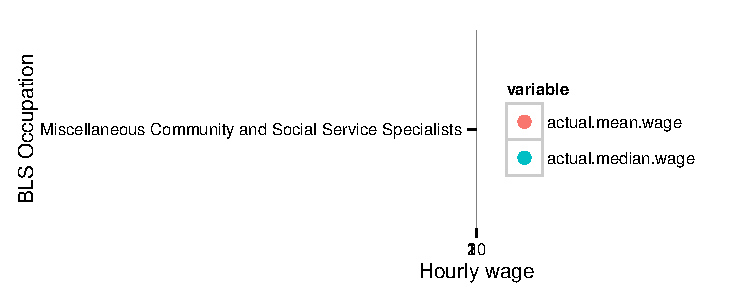
\includegraphics[width=\maxwidth]{figure/unnamed-chunk-247} 

}


\newpage\section{Childcare Workers}\textbf{Occupation code:} 39-9010\newline\textbf{Typical entry education:} High school diploma or equivalent\newline\textbf{Detailed occupations:}\newline1. (39-9011)  \href{http://www.bls.gov/oes/current/oes399011.htm}{Childcare Workers}\newline% latex table generated in R 3.0.2 by xtable 1.7-1 package
% Sun Nov 24 09:11:58 2013
\begin{table}[ht]
\centering
{\footnotesize
\begin{tabular}{ll|rrr}
 \textbf{Variable} & \textbf{Levels} & $\mathbf{n}$ & $\mathbf{\%}$ & $\mathbf{\sum \%}$ \\ 
  \hline
know.job &  & 0 & 0.0 & 0.0 \\ 
   & Maybe & 1 & 3.3 & 3.3 \\ 
   & No & 1 & 3.3 & 6.7 \\ 
   & Yes & 28 & 93.3 & 100.0 \\ 
   \hline
 & all & 30 & 100.0 &  \\ 
   \hline
\hline
social.knowledge & 0 & 12 & 40.0 & 40.0 \\ 
   & 1 & 7 & 23.3 & 63.3 \\ 
   & 2 & 8 & 26.7 & 90.0 \\ 
   & 3-10 & 3 & 10.0 & 100.0 \\ 
   & 10-plus & 0 & 0.0 & 100.0 \\ 
   \hline
 & all & 30 & 100.0 &  \\ 
   \hline
\hline
Answer.volume\_trend &  & 0 & 0.0 & 0.0 \\ 
   & GoDown & 0 & 0.0 & 0.0 \\ 
   & GoUp & 20 & 66.7 & 66.7 \\ 
   & StayTheSame & 10 & 33.3 & 100.0 \\ 
   \hline
 & all & 30 & 100.0 &  \\ 
   \hline
\hline
Answer.wage\_trend &  & 0 & 0.0 & 0.0 \\ 
   & GoDown & 2 & 6.7 & 6.7 \\ 
   & GoUp & 13 & 43.3 & 50.0 \\ 
   & StayTheSame & 15 & 50.0 & 100.0 \\ 
   \hline
 & all & 30 & 100.0 &  \\ 
   \hline
\hline
\end{tabular}
}
\caption{Summary statistics, nominal variables (MTurk data)} 
\label{tab1:39-9010}
\end{table}
% latex table generated in R 3.0.2 by xtable 1.7-1 package
% Sun Nov 24 09:11:58 2013
\begin{table}[ht]
\centering
{\footnotesize
\begin{tabular}{lrrrrrrrrrr}
 \textbf{Variable} & $\mathbf{n}$ & \textbf{Min} & $\mathbf{q_1}$ & $\mathbf{\widetilde{x}}$ & $\mathbf{\bar{x}}$ & $\mathbf{q_3}$ & \textbf{Max} & $\mathbf{s}$ & \textbf{IQR} & \textbf{\#NA} \\ 
  \hline
wage & 30 & 9 & 10 & 12 & 12.6 & 14 & 20 & 2.7 & 4 & 0 \\ 
  \end{tabular}
}
\caption{Summary statistics, continuous variables (MTurk data)} 
\label{tab2:39-9010}
\end{table}


{\centering 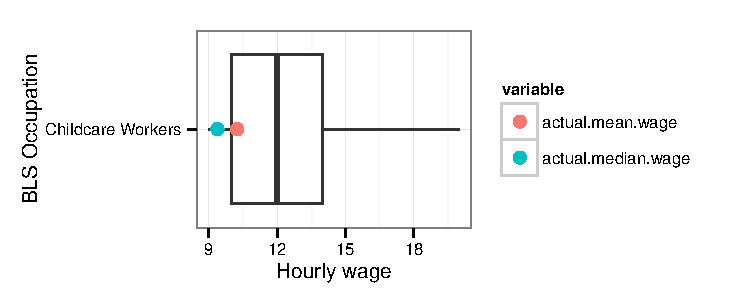
\includegraphics[width=\maxwidth]{figure/unnamed-chunk-248} 

}


\newpage\section{Physicians and Surgeons}\textbf{Occupation code:} 29-1060\newline\textbf{Typical entry education:} Doctoral or professional degree\newline\textbf{Detailed occupations:}\newline1. (29-1061)  \href{http://www.bls.gov/oes/current/oes291061.htm}{Anesthesiologists}\newline2. (29-1062)  \href{http://www.bls.gov/oes/current/oes291062.htm}{Family and General Practitioners}\newline3. (29-1063)  \href{http://www.bls.gov/oes/current/oes291063.htm}{Internists, General}\newline4. (29-1064)  \href{http://www.bls.gov/oes/current/oes291064.htm}{Obstetricians and Gynecologists}\newline5. (29-1065)  \href{http://www.bls.gov/oes/current/oes291065.htm}{Pediatricians, General}\newline6. (29-1066)  \href{http://www.bls.gov/oes/current/oes291066.htm}{Psychiatrists}\newline7. (29-1067)  \href{http://www.bls.gov/oes/current/oes291067.htm}{Surgeons}\newline8. (29-1069)  \href{http://www.bls.gov/oes/current/oes291069.htm}{Physicians and Surgeons, All Other}\newline% latex table generated in R 3.0.2 by xtable 1.7-1 package
% Sun Nov 24 09:11:58 2013
\begin{table}[ht]
\centering
{\footnotesize
\begin{tabular}{ll|rrr}
 \textbf{Variable} & \textbf{Levels} & $\mathbf{n}$ & $\mathbf{\%}$ & $\mathbf{\sum \%}$ \\ 
  \hline
know.job &  & 0 & 0.0 & 0.0 \\ 
   & Maybe & 0 & 0.0 & 0.0 \\ 
   & No & 1 & 3.3 & 3.3 \\ 
   & Yes & 29 & 96.7 & 100.0 \\ 
   \hline
 & all & 30 & 100.0 &  \\ 
   \hline
\hline
social.knowledge & 0 & 15 & 50.0 & 50.0 \\ 
   & 1 & 9 & 30.0 & 80.0 \\ 
   & 2 & 1 & 3.3 & 83.3 \\ 
   & 3-10 & 4 & 13.3 & 96.7 \\ 
   & 10-plus & 1 & 3.3 & 100.0 \\ 
   \hline
 & all & 30 & 100.0 &  \\ 
   \hline
\hline
Answer.volume\_trend &  & 0 & 0.0 & 0.0 \\ 
   & GoDown & 7 & 23.3 & 23.3 \\ 
   & GoUp & 12 & 40.0 & 63.3 \\ 
   & StayTheSame & 11 & 36.7 & 100.0 \\ 
   \hline
 & all & 30 & 100.0 &  \\ 
   \hline
\hline
Answer.wage\_trend &  & 0 & 0.0 & 0.0 \\ 
   & GoDown & 5 & 16.7 & 16.7 \\ 
   & GoUp & 19 & 63.3 & 80.0 \\ 
   & StayTheSame & 6 & 20.0 & 100.0 \\ 
   \hline
 & all & 30 & 100.0 &  \\ 
   \hline
\hline
\end{tabular}
}
\caption{Summary statistics, nominal variables (MTurk data)} 
\label{tab1:29-1060}
\end{table}
% latex table generated in R 3.0.2 by xtable 1.7-1 package
% Sun Nov 24 09:11:58 2013
\begin{table}[ht]
\centering
{\footnotesize
\begin{tabular}{lrrrrrrrrrr}
 \textbf{Variable} & $\mathbf{n}$ & \textbf{Min} & $\mathbf{q_1}$ & $\mathbf{\widetilde{x}}$ & $\mathbf{\bar{x}}$ & $\mathbf{q_3}$ & \textbf{Max} & $\mathbf{s}$ & \textbf{IQR} & \textbf{\#NA} \\ 
  \hline
wage & 30 & 32 & 70 & 70 & 64.9 & 70 & 70 & 11.7 & 0 & 0 \\ 
  \end{tabular}
}
\caption{Summary statistics, continuous variables (MTurk data)} 
\label{tab2:29-1060}
\end{table}


{\centering 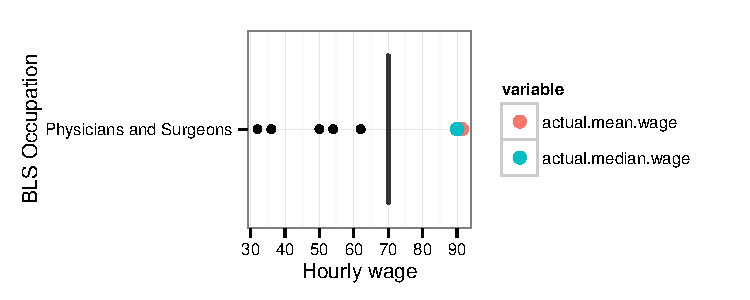
\includegraphics[width=\maxwidth]{figure/unnamed-chunk-249} 

}


\newpage\section{Database and Systems Administrators and Network Architects}\textbf{Occupation code:} 15-1140\newline\textbf{Typical entry education:} Bachelor's degree\newline\textbf{Detailed occupations:}\newline1. (15-1141)  \href{http://www.bls.gov/oes/current/oes151141.htm}{Database Administrators}\newline2. (15-1142)  \href{http://www.bls.gov/oes/current/oes151142.htm}{Network and Computer Systems Administrators}\newline3. (15-1143)  \href{http://www.bls.gov/oes/current/oes151143.htm}{Computer Network Architects}\newline% latex table generated in R 3.0.2 by xtable 1.7-1 package
% Sun Nov 24 09:11:59 2013
\begin{table}[ht]
\centering
{\footnotesize
\begin{tabular}{ll|rrr}
 \textbf{Variable} & \textbf{Levels} & $\mathbf{n}$ & $\mathbf{\%}$ & $\mathbf{\sum \%}$ \\ 
  \hline
know.job &  & 0 & 0.0 & 0.0 \\ 
   & Maybe & 10 & 33.3 & 33.3 \\ 
   & No & 3 & 10.0 & 43.3 \\ 
   & Yes & 17 & 56.7 & 100.0 \\ 
   \hline
 & all & 30 & 100.0 &  \\ 
   \hline
\hline
social.knowledge & 0 & 16 & 53.3 & 53.3 \\ 
   & 1 & 8 & 26.7 & 80.0 \\ 
   & 2 & 5 & 16.7 & 96.7 \\ 
   & 3-10 & 1 & 3.3 & 100.0 \\ 
   & 10-plus & 0 & 0.0 & 100.0 \\ 
   \hline
 & all & 30 & 100.0 &  \\ 
   \hline
\hline
Answer.volume\_trend &  & 0 & 0.0 & 0.0 \\ 
   & GoDown & 1 & 3.3 & 3.3 \\ 
   & GoUp & 27 & 90.0 & 93.3 \\ 
   & StayTheSame & 2 & 6.7 & 100.0 \\ 
   \hline
 & all & 30 & 100.0 &  \\ 
   \hline
\hline
Answer.wage\_trend &  & 0 & 0.0 & 0.0 \\ 
   & GoDown & 1 & 3.3 & 3.3 \\ 
   & GoUp & 23 & 76.7 & 80.0 \\ 
   & StayTheSame & 6 & 20.0 & 100.0 \\ 
   \hline
 & all & 30 & 100.0 &  \\ 
   \hline
\hline
\end{tabular}
}
\caption{Summary statistics, nominal variables (MTurk data)} 
\label{tab1:15-1140}
\end{table}
% latex table generated in R 3.0.2 by xtable 1.7-1 package
% Sun Nov 24 09:11:59 2013
\begin{table}[ht]
\centering
{\footnotesize
\begin{tabular}{lrrrrrrrrrr}
 \textbf{Variable} & $\mathbf{n}$ & \textbf{Min} & $\mathbf{q_1}$ & $\mathbf{\widetilde{x}}$ & $\mathbf{\bar{x}}$ & $\mathbf{q_3}$ & \textbf{Max} & $\mathbf{s}$ & \textbf{IQR} & \textbf{\#NA} \\ 
  \hline
wage & 30 & 12 & 20 & 24 & 26.3 & 32 & 50 & 7.7 & 12 & 0 \\ 
  \end{tabular}
}
\caption{Summary statistics, continuous variables (MTurk data)} 
\label{tab2:15-1140}
\end{table}


{\centering 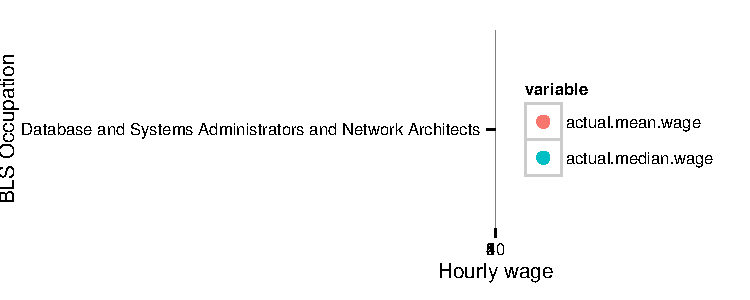
\includegraphics[width=\maxwidth]{figure/unnamed-chunk-250} 

}


\newpage\section{Counselors}\textbf{Occupation code:} 21-1010\newline\textbf{Typical entry education:} High school diploma or equivalent\newline\textbf{Detailed occupations:}\newline1. (21-1011)  \href{http://www.bls.gov/oes/current/oes211011.htm}{Substance Abuse and Behavioral Disorder Counselors}\newline2. (21-1012)  \href{http://www.bls.gov/oes/current/oes211012.htm}{Educational, Guidance, School, and Vocational Counselors}\newline3. (21-1013)  \href{http://www.bls.gov/oes/current/oes211013.htm}{Marriage and Family Therapists}\newline4. (21-1014)  \href{http://www.bls.gov/oes/current/oes211014.htm}{Mental Health Counselors}\newline5. (21-1015)  \href{http://www.bls.gov/oes/current/oes211015.htm}{Rehabilitation Counselors}\newline6. (21-1019)  \href{http://www.bls.gov/oes/current/oes211019.htm}{Counselors, All Other}\newline% latex table generated in R 3.0.2 by xtable 1.7-1 package
% Sun Nov 24 09:11:59 2013
\begin{table}[ht]
\centering
{\footnotesize
\begin{tabular}{ll|rrr}
 \textbf{Variable} & \textbf{Levels} & $\mathbf{n}$ & $\mathbf{\%}$ & $\mathbf{\sum \%}$ \\ 
  \hline
know.job &  & 1 & 3.3 & 3.3 \\ 
   & Maybe & 3 & 10.0 & 13.3 \\ 
   & No & 1 & 3.3 & 16.7 \\ 
   & Yes & 25 & 83.3 & 100.0 \\ 
   \hline
 & all & 30 & 100.0 &  \\ 
   \hline
\hline
social.knowledge & 0 & 17 & 56.7 & 56.7 \\ 
   & 1 & 8 & 26.7 & 83.3 \\ 
   & 2 & 3 & 10.0 & 93.3 \\ 
   & 3-10 & 2 & 6.7 & 100.0 \\ 
   & 10-plus & 0 & 0.0 & 100.0 \\ 
   \hline
 & all & 30 & 100.0 &  \\ 
   \hline
\hline
Answer.volume\_trend &  & 0 & 0.0 & 0.0 \\ 
   & GoDown & 2 & 6.7 & 6.7 \\ 
   & GoUp & 16 & 53.3 & 60.0 \\ 
   & StayTheSame & 12 & 40.0 & 100.0 \\ 
   \hline
 & all & 30 & 100.0 &  \\ 
   \hline
\hline
Answer.wage\_trend &  & 0 & 0.0 & 0.0 \\ 
   & GoDown & 0 & 0.0 & 0.0 \\ 
   & GoUp & 18 & 60.0 & 60.0 \\ 
   & StayTheSame & 12 & 40.0 & 100.0 \\ 
   \hline
 & all & 30 & 100.0 &  \\ 
   \hline
\hline
\end{tabular}
}
\caption{Summary statistics, nominal variables (MTurk data)} 
\label{tab1:21-1010}
\end{table}
% latex table generated in R 3.0.2 by xtable 1.7-1 package
% Sun Nov 24 09:11:59 2013
\begin{table}[ht]
\centering
{\footnotesize
\begin{tabular}{lrrrrrrrrrr}
 \textbf{Variable} & $\mathbf{n}$ & \textbf{Min} & $\mathbf{q_1}$ & $\mathbf{\widetilde{x}}$ & $\mathbf{\bar{x}}$ & $\mathbf{q_3}$ & \textbf{Max} & $\mathbf{s}$ & \textbf{IQR} & \textbf{\#NA} \\ 
  \hline
wage & 30 & 16 & 18.5 & 20 & 24.6 & 27 & 70 & 11.5 & 8.5 & 0 \\ 
  \end{tabular}
}
\caption{Summary statistics, continuous variables (MTurk data)} 
\label{tab2:21-1010}
\end{table}


{\centering \includegraphics[width=\maxwidth]{figure/unnamed-chunk-251} 

}


\newpage\section{Lawyers and Judicial Law Clerks}\textbf{Occupation code:} 23-1010\newline\textbf{Typical entry education:} Doctoral or professional degree\newline\textbf{Detailed occupations:}\newline1. (23-1011)  \href{http://www.bls.gov/oes/current/oes231011.htm}{Lawyers}\newline2. (23-1012)  \href{http://www.bls.gov/oes/current/oes231012.htm}{Judicial Law Clerks}\newline% latex table generated in R 3.0.2 by xtable 1.7-1 package
% Sun Nov 24 09:12:00 2013
\begin{table}[ht]
\centering
{\footnotesize
\begin{tabular}{ll|rrr}
 \textbf{Variable} & \textbf{Levels} & $\mathbf{n}$ & $\mathbf{\%}$ & $\mathbf{\sum \%}$ \\ 
  \hline
know.job &  & 1 & 3.3 & 3.3 \\ 
   & Maybe & 3 & 10.0 & 13.3 \\ 
   & No & 0 & 0.0 & 13.3 \\ 
   & Yes & 26 & 86.7 & 100.0 \\ 
   \hline
 & all & 30 & 100.0 &  \\ 
   \hline
\hline
social.knowledge & 0 & 12 & 41.4 & 41.4 \\ 
   & 1 & 6 & 20.7 & 62.1 \\ 
   & 2 & 6 & 20.7 & 82.8 \\ 
   & 3-10 & 4 & 13.8 & 96.6 \\ 
   & 10-plus & 1 & 3.5 & 100.0 \\ 
   \hline
 & all & 29 & 100.0 &  \\ 
   \hline
\hline
Answer.volume\_trend &  & 0 & 0.0 & 0.0 \\ 
   & GoDown & 2 & 6.7 & 6.7 \\ 
   & GoUp & 15 & 50.0 & 56.7 \\ 
   & StayTheSame & 13 & 43.3 & 100.0 \\ 
   \hline
 & all & 30 & 100.0 &  \\ 
   \hline
\hline
Answer.wage\_trend &  & 0 & 0.0 & 0.0 \\ 
   & GoDown & 1 & 3.3 & 3.3 \\ 
   & GoUp & 24 & 80.0 & 83.3 \\ 
   & StayTheSame & 5 & 16.7 & 100.0 \\ 
   \hline
 & all & 30 & 100.0 &  \\ 
   \hline
\hline
\end{tabular}
}
\caption{Summary statistics, nominal variables (MTurk data)} 
\label{tab1:23-1010}
\end{table}
% latex table generated in R 3.0.2 by xtable 1.7-1 package
% Sun Nov 24 09:12:00 2013
\begin{table}[ht]
\centering
{\footnotesize
\begin{tabular}{lrrrrrrrrrr}
 \textbf{Variable} & $\mathbf{n}$ & \textbf{Min} & $\mathbf{q_1}$ & $\mathbf{\widetilde{x}}$ & $\mathbf{\bar{x}}$ & $\mathbf{q_3}$ & \textbf{Max} & $\mathbf{s}$ & \textbf{IQR} & \textbf{\#NA} \\ 
  \hline
wage & 30 & 16 & 39.5 & 50 & 51.9 & 70 & 70 & 18.1 & 30.5 & 0 \\ 
  \end{tabular}
}
\caption{Summary statistics, continuous variables (MTurk data)} 
\label{tab2:23-1010}
\end{table}


{\centering \includegraphics[width=\maxwidth]{figure/unnamed-chunk-252} 

}


\newpage\section{Therapists}\textbf{Occupation code:} 29-1120\newline\textbf{Typical entry education:} Associate's degree\newline\textbf{Detailed occupations:}\newline1. (29-1122)  \href{http://www.bls.gov/oes/current/oes291122.htm}{Occupational Therapists}\newline2. (29-1123)  \href{http://www.bls.gov/oes/current/oes291123.htm}{Physical Therapists}\newline3. (29-1124)  \href{http://www.bls.gov/oes/current/oes291124.htm}{Radiation Therapists}\newline4. (29-1125)  \href{http://www.bls.gov/oes/current/oes291125.htm}{Recreational Therapists}\newline5. (29-1126)  \href{http://www.bls.gov/oes/current/oes291126.htm}{Respiratory Therapists}\newline6. (29-1127)  \href{http://www.bls.gov/oes/current/oes291127.htm}{Speech-Language Pathologists}\newline7. (29-1128)  \href{http://www.bls.gov/oes/current/oes291128.htm}{Exercise Physiologists}\newline8. (29-1129)  \href{http://www.bls.gov/oes/current/oes291129.htm}{Therapists, All Other}\newline% latex table generated in R 3.0.2 by xtable 1.7-1 package
% Sun Nov 24 09:12:00 2013
\begin{table}[ht]
\centering
{\footnotesize
\begin{tabular}{ll|rrr}
 \textbf{Variable} & \textbf{Levels} & $\mathbf{n}$ & $\mathbf{\%}$ & $\mathbf{\sum \%}$ \\ 
  \hline
know.job &  & 0 & 0.0 & 0.0 \\ 
   & Maybe & 1 & 3.3 & 3.3 \\ 
   & No & 2 & 6.7 & 10.0 \\ 
   & Yes & 27 & 90.0 & 100.0 \\ 
   \hline
 & all & 30 & 100.0 &  \\ 
   \hline
\hline
social.knowledge & 0 & 21 & 70.0 & 70.0 \\ 
   & 1 & 5 & 16.7 & 86.7 \\ 
   & 2 & 3 & 10.0 & 96.7 \\ 
   & 3-10 & 1 & 3.3 & 100.0 \\ 
   & 10-plus & 0 & 0.0 & 100.0 \\ 
   \hline
 & all & 30 & 100.0 &  \\ 
   \hline
\hline
Answer.volume\_trend &  & 0 & 0.0 & 0.0 \\ 
   & GoDown & 3 & 10.0 & 10.0 \\ 
   & GoUp & 16 & 53.3 & 63.3 \\ 
   & StayTheSame & 11 & 36.7 & 100.0 \\ 
   \hline
 & all & 30 & 100.0 &  \\ 
   \hline
\hline
Answer.wage\_trend &  & 0 & 0.0 & 0.0 \\ 
   & GoDown & 0 & 0.0 & 0.0 \\ 
   & GoUp & 22 & 73.3 & 73.3 \\ 
   & StayTheSame & 8 & 26.7 & 100.0 \\ 
   \hline
 & all & 30 & 100.0 &  \\ 
   \hline
\hline
\end{tabular}
}
\caption{Summary statistics, nominal variables (MTurk data)} 
\label{tab1:29-1120}
\end{table}
% latex table generated in R 3.0.2 by xtable 1.7-1 package
% Sun Nov 24 09:12:00 2013
\begin{table}[ht]
\centering
{\footnotesize
\begin{tabular}{lrrrrrrrrrr}
 \textbf{Variable} & $\mathbf{n}$ & \textbf{Min} & $\mathbf{q_1}$ & $\mathbf{\widetilde{x}}$ & $\mathbf{\bar{x}}$ & $\mathbf{q_3}$ & \textbf{Max} & $\mathbf{s}$ & \textbf{IQR} & \textbf{\#NA} \\ 
  \hline
wage & 30 & 18 & 25 & 34 & 37.5 & 50 & 70 & 14.1 & 25 & 0 \\ 
  \end{tabular}
}
\caption{Summary statistics, continuous variables (MTurk data)} 
\label{tab2:29-1120}
\end{table}


{\centering \includegraphics[width=\maxwidth]{figure/unnamed-chunk-253} 

}


\newpage\section{Social Workers}\textbf{Occupation code:} 21-1020\newline\textbf{Typical entry education:} Bachelor's degree\newline\textbf{Detailed occupations:}\newline1. (21-1021)  \href{http://www.bls.gov/oes/current/oes211021.htm}{Child, Family, and School Social Workers}\newline2. (21-1022)  \href{http://www.bls.gov/oes/current/oes211022.htm}{Healthcare Social Workers}\newline3. (21-1023)  \href{http://www.bls.gov/oes/current/oes211023.htm}{Mental Health and Substance Abuse Social Workers}\newline4. (21-1029)  \href{http://www.bls.gov/oes/current/oes211029.htm}{Social Workers, All Other}\newline% latex table generated in R 3.0.2 by xtable 1.7-1 package
% Sun Nov 24 09:12:01 2013
\begin{table}[ht]
\centering
{\footnotesize
\begin{tabular}{ll|rrr}
 \textbf{Variable} & \textbf{Levels} & $\mathbf{n}$ & $\mathbf{\%}$ & $\mathbf{\sum \%}$ \\ 
  \hline
know.job &  & 0 & 0.0 & 0.0 \\ 
   & Maybe & 0 & 0.0 & 0.0 \\ 
   & No & 1 & 3.3 & 3.3 \\ 
   & Yes & 29 & 96.7 & 100.0 \\ 
   \hline
 & all & 30 & 100.0 &  \\ 
   \hline
\hline
social.knowledge & 0 & 18 & 60.0 & 60.0 \\ 
   & 1 & 7 & 23.3 & 83.3 \\ 
   & 2 & 3 & 10.0 & 93.3 \\ 
   & 3-10 & 2 & 6.7 & 100.0 \\ 
   & 10-plus & 0 & 0.0 & 100.0 \\ 
   \hline
 & all & 30 & 100.0 &  \\ 
   \hline
\hline
Answer.volume\_trend &  & 0 & 0.0 & 0.0 \\ 
   & GoDown & 1 & 3.3 & 3.3 \\ 
   & GoUp & 14 & 46.7 & 50.0 \\ 
   & StayTheSame & 15 & 50.0 & 100.0 \\ 
   \hline
 & all & 30 & 100.0 &  \\ 
   \hline
\hline
Answer.wage\_trend &  & 0 & 0.0 & 0.0 \\ 
   & GoDown & 3 & 10.0 & 10.0 \\ 
   & GoUp & 12 & 40.0 & 50.0 \\ 
   & StayTheSame & 15 & 50.0 & 100.0 \\ 
   \hline
 & all & 30 & 100.0 &  \\ 
   \hline
\hline
\end{tabular}
}
\caption{Summary statistics, nominal variables (MTurk data)} 
\label{tab1:21-1020}
\end{table}
% latex table generated in R 3.0.2 by xtable 1.7-1 package
% Sun Nov 24 09:12:01 2013
\begin{table}[ht]
\centering
{\footnotesize
\begin{tabular}{lrrrrrrrrrr}
 \textbf{Variable} & $\mathbf{n}$ & \textbf{Min} & $\mathbf{q_1}$ & $\mathbf{\widetilde{x}}$ & $\mathbf{\bar{x}}$ & $\mathbf{q_3}$ & \textbf{Max} & $\mathbf{s}$ & \textbf{IQR} & \textbf{\#NA} \\ 
  \hline
wage & 30 & 5 & 12.5 & 16 & 17.1 & 20 & 32 & 5.9 & 7.5 & 0 \\ 
  \end{tabular}
}
\caption{Summary statistics, continuous variables (MTurk data)} 
\label{tab2:21-1020}
\end{table}


{\centering \includegraphics[width=\maxwidth]{figure/unnamed-chunk-254} 

}


\newpage\section{First-Line Supervisors of Production and Operating Workers}\textbf{Occupation code:} 51-1010\newline\textbf{Typical entry education:} Postsecondary non-degree award\newline\textbf{Detailed occupations:}\newline1. (51-1011)  \href{http://www.bls.gov/oes/current/oes511011.htm}{First-Line Supervisors of Production and Operating Workers}\newline% latex table generated in R 3.0.2 by xtable 1.7-1 package
% Sun Nov 24 09:12:01 2013
\begin{table}[ht]
\centering
{\footnotesize
\begin{tabular}{ll|rrr}
 \textbf{Variable} & \textbf{Levels} & $\mathbf{n}$ & $\mathbf{\%}$ & $\mathbf{\sum \%}$ \\ 
  \hline
know.job &  & 0 & 0.0 & 0.0 \\ 
   & Maybe & 12 & 40.0 & 40.0 \\ 
   & No & 5 & 16.7 & 56.7 \\ 
   & Yes & 13 & 43.3 & 100.0 \\ 
   \hline
 & all & 30 & 100.0 &  \\ 
   \hline
\hline
social.knowledge & 0 & 19 & 63.3 & 63.3 \\ 
   & 1 & 7 & 23.3 & 86.7 \\ 
   & 2 & 1 & 3.3 & 90.0 \\ 
   & 3-10 & 2 & 6.7 & 96.7 \\ 
   & 10-plus & 1 & 3.3 & 100.0 \\ 
   \hline
 & all & 30 & 100.0 &  \\ 
   \hline
\hline
Answer.volume\_trend &  & 0 & 0.0 & 0.0 \\ 
   & GoDown & 7 & 23.3 & 23.3 \\ 
   & GoUp & 6 & 20.0 & 43.3 \\ 
   & StayTheSame & 17 & 56.7 & 100.0 \\ 
   \hline
 & all & 30 & 100.0 &  \\ 
   \hline
\hline
Answer.wage\_trend &  & 0 & 0.0 & 0.0 \\ 
   & GoDown & 4 & 13.3 & 13.3 \\ 
   & GoUp & 12 & 40.0 & 53.3 \\ 
   & StayTheSame & 14 & 46.7 & 100.0 \\ 
   \hline
 & all & 30 & 100.0 &  \\ 
   \hline
\hline
\end{tabular}
}
\caption{Summary statistics, nominal variables (MTurk data)} 
\label{tab1:51-1010}
\end{table}
% latex table generated in R 3.0.2 by xtable 1.7-1 package
% Sun Nov 24 09:12:01 2013
\begin{table}[ht]
\centering
{\footnotesize
\begin{tabular}{lrrrrrrrrrr}
 \textbf{Variable} & $\mathbf{n}$ & \textbf{Min} & $\mathbf{q_1}$ & $\mathbf{\widetilde{x}}$ & $\mathbf{\bar{x}}$ & $\mathbf{q_3}$ & \textbf{Max} & $\mathbf{s}$ & \textbf{IQR} & \textbf{\#NA} \\ 
  \hline
wage & 30 & 10 & 14 & 16 & 18 & 19.5 & 50 & 7.7 & 5.5 & 0 \\ 
  \end{tabular}
}
\caption{Summary statistics, continuous variables (MTurk data)} 
\label{tab2:51-1010}
\end{table}


{\centering \includegraphics[width=\maxwidth]{figure/unnamed-chunk-255} 

}


\newpage\section{Carpenters}\textbf{Occupation code:} 47-2030\newline\textbf{Typical entry education:} High school diploma or equivalent\newline\textbf{Detailed occupations:}\newline1. (47-2031)  \href{http://www.bls.gov/oes/current/oes472031.htm}{Carpenters}\newline% latex table generated in R 3.0.2 by xtable 1.7-1 package
% Sun Nov 24 09:12:02 2013
\begin{table}[ht]
\centering
{\footnotesize
\begin{tabular}{ll|rrr}
 \textbf{Variable} & \textbf{Levels} & $\mathbf{n}$ & $\mathbf{\%}$ & $\mathbf{\sum \%}$ \\ 
  \hline
know.job &  & 0 & 0.0 & 0.0 \\ 
   & Maybe & 0 & 0.0 & 0.0 \\ 
   & No & 1 & 3.3 & 3.3 \\ 
   & Yes & 29 & 96.7 & 100.0 \\ 
   \hline
 & all & 30 & 100.0 &  \\ 
   \hline
\hline
social.knowledge & 0 & 10 & 33.3 & 33.3 \\ 
   & 1 & 11 & 36.7 & 70.0 \\ 
   & 2 & 3 & 10.0 & 80.0 \\ 
   & 3-10 & 5 & 16.7 & 96.7 \\ 
   & 10-plus & 1 & 3.3 & 100.0 \\ 
   \hline
 & all & 30 & 100.0 &  \\ 
   \hline
\hline
Answer.volume\_trend &  & 0 & 0.0 & 0.0 \\ 
   & GoDown & 8 & 26.7 & 26.7 \\ 
   & GoUp & 9 & 30.0 & 56.7 \\ 
   & StayTheSame & 13 & 43.3 & 100.0 \\ 
   \hline
 & all & 30 & 100.0 &  \\ 
   \hline
\hline
Answer.wage\_trend &  & 0 & 0.0 & 0.0 \\ 
   & GoDown & 0 & 0.0 & 0.0 \\ 
   & GoUp & 18 & 60.0 & 60.0 \\ 
   & StayTheSame & 12 & 40.0 & 100.0 \\ 
   \hline
 & all & 30 & 100.0 &  \\ 
   \hline
\hline
\end{tabular}
}
\caption{Summary statistics, nominal variables (MTurk data)} 
\label{tab1:47-2030}
\end{table}
% latex table generated in R 3.0.2 by xtable 1.7-1 package
% Sun Nov 24 09:12:02 2013
\begin{table}[ht]
\centering
{\footnotesize
\begin{tabular}{lrrrrrrrrrr}
 \textbf{Variable} & $\mathbf{n}$ & \textbf{Min} & $\mathbf{q_1}$ & $\mathbf{\widetilde{x}}$ & $\mathbf{\bar{x}}$ & $\mathbf{q_3}$ & \textbf{Max} & $\mathbf{s}$ & \textbf{IQR} & \textbf{\#NA} \\ 
  \hline
wage & 30 & 12 & 16.5 & 19 & 20.7 & 23 & 50 & 7.9 & 6.5 & 0 \\ 
  \end{tabular}
}
\caption{Summary statistics, continuous variables (MTurk data)} 
\label{tab2:47-2030}
\end{table}


{\centering \includegraphics[width=\maxwidth]{figure/unnamed-chunk-256} 

}


\newpage\section{Computer and Information Analysts}\textbf{Occupation code:} 15-1120\newline\textbf{Typical entry education:} Bachelor's degree\newline\textbf{Detailed occupations:}\newline1. (15-1121)  \href{http://www.bls.gov/oes/current/oes151121.htm}{Computer Systems Analysts}\newline2. (15-1122)  \href{http://www.bls.gov/oes/current/oes151122.htm}{Information Security Analysts}\newline% latex table generated in R 3.0.2 by xtable 1.7-1 package
% Sun Nov 24 09:12:02 2013
\begin{table}[ht]
\centering
{\footnotesize
\begin{tabular}{ll|rrr}
 \textbf{Variable} & \textbf{Levels} & $\mathbf{n}$ & $\mathbf{\%}$ & $\mathbf{\sum \%}$ \\ 
  \hline
know.job &  & 0 & 0.0 & 0.0 \\ 
   & Maybe & 5 & 16.7 & 16.7 \\ 
   & No & 3 & 10.0 & 26.7 \\ 
   & Yes & 22 & 73.3 & 100.0 \\ 
   \hline
 & all & 30 & 100.0 &  \\ 
   \hline
\hline
social.knowledge & 0 & 13 & 43.3 & 43.3 \\ 
   & 1 & 6 & 20.0 & 63.3 \\ 
   & 2 & 4 & 13.3 & 76.7 \\ 
   & 3-10 & 6 & 20.0 & 96.7 \\ 
   & 10-plus & 1 & 3.3 & 100.0 \\ 
   \hline
 & all & 30 & 100.0 &  \\ 
   \hline
\hline
Answer.volume\_trend &  & 0 & 0.0 & 0.0 \\ 
   & GoDown & 1 & 3.3 & 3.3 \\ 
   & GoUp & 27 & 90.0 & 93.3 \\ 
   & StayTheSame & 2 & 6.7 & 100.0 \\ 
   \hline
 & all & 30 & 100.0 &  \\ 
   \hline
\hline
Answer.wage\_trend &  & 0 & 0.0 & 0.0 \\ 
   & GoDown & 1 & 3.3 & 3.3 \\ 
   & GoUp & 23 & 76.7 & 80.0 \\ 
   & StayTheSame & 6 & 20.0 & 100.0 \\ 
   \hline
 & all & 30 & 100.0 &  \\ 
   \hline
\hline
\end{tabular}
}
\caption{Summary statistics, nominal variables (MTurk data)} 
\label{tab1:15-1120}
\end{table}
% latex table generated in R 3.0.2 by xtable 1.7-1 package
% Sun Nov 24 09:12:02 2013
\begin{table}[ht]
\centering
{\footnotesize
\begin{tabular}{lrrrrrrrrrr}
 \textbf{Variable} & $\mathbf{n}$ & \textbf{Min} & $\mathbf{q_1}$ & $\mathbf{\widetilde{x}}$ & $\mathbf{\bar{x}}$ & $\mathbf{q_3}$ & \textbf{Max} & $\mathbf{s}$ & \textbf{IQR} & \textbf{\#NA} \\ 
  \hline
wage & 30 & 12 & 20 & 24 & 25.9 & 32 & 50 & 8.3 & 12 & 0 \\ 
  \end{tabular}
}
\caption{Summary statistics, continuous variables (MTurk data)} 
\label{tab2:15-1120}
\end{table}


{\centering \includegraphics[width=\maxwidth]{figure/unnamed-chunk-257} 

}


\newpage\section{Recreation and Fitness Workers}\textbf{Occupation code:} 39-9030\newline\textbf{Typical entry education:} High school diploma or equivalent\newline\textbf{Detailed occupations:}\newline1. (39-9031)  \href{http://www.bls.gov/oes/current/oes399031.htm}{Fitness Trainers and Aerobics Instructors}\newline2. (39-9032)  \href{http://www.bls.gov/oes/current/oes399032.htm}{Recreation Workers}\newline% latex table generated in R 3.0.2 by xtable 1.7-1 package
% Sun Nov 24 09:12:03 2013
\begin{table}[ht]
\centering
{\footnotesize
\begin{tabular}{ll|rrr}
 \textbf{Variable} & \textbf{Levels} & $\mathbf{n}$ & $\mathbf{\%}$ & $\mathbf{\sum \%}$ \\ 
  \hline
know.job &  & 0 & 0.0 & 0.0 \\ 
   & Maybe & 6 & 20.0 & 20.0 \\ 
   & No & 4 & 13.3 & 33.3 \\ 
   & Yes & 20 & 66.7 & 100.0 \\ 
   \hline
 & all & 30 & 100.0 &  \\ 
   \hline
\hline
social.knowledge & 0 & 21 & 70.0 & 70.0 \\ 
   & 1 & 3 & 10.0 & 80.0 \\ 
   & 2 & 4 & 13.3 & 93.3 \\ 
   & 3-10 & 2 & 6.7 & 100.0 \\ 
   & 10-plus & 0 & 0.0 & 100.0 \\ 
   \hline
 & all & 30 & 100.0 &  \\ 
   \hline
\hline
Answer.volume\_trend &  & 0 & 0.0 & 0.0 \\ 
   & GoDown & 5 & 16.7 & 16.7 \\ 
   & GoUp & 15 & 50.0 & 66.7 \\ 
   & StayTheSame & 10 & 33.3 & 100.0 \\ 
   \hline
 & all & 30 & 100.0 &  \\ 
   \hline
\hline
Answer.wage\_trend &  & 0 & 0.0 & 0.0 \\ 
   & GoDown & 2 & 6.7 & 6.7 \\ 
   & GoUp & 20 & 66.7 & 73.3 \\ 
   & StayTheSame & 8 & 26.7 & 100.0 \\ 
   \hline
 & all & 30 & 100.0 &  \\ 
   \hline
\hline
\end{tabular}
}
\caption{Summary statistics, nominal variables (MTurk data)} 
\label{tab1:39-9030}
\end{table}
% latex table generated in R 3.0.2 by xtable 1.7-1 package
% Sun Nov 24 09:12:03 2013
\begin{table}[ht]
\centering
{\footnotesize
\begin{tabular}{lrrrrrrrrrr}
 \textbf{Variable} & $\mathbf{n}$ & \textbf{Min} & $\mathbf{q_1}$ & $\mathbf{\widetilde{x}}$ & $\mathbf{\bar{x}}$ & $\mathbf{q_3}$ & \textbf{Max} & $\mathbf{s}$ & \textbf{IQR} & \textbf{\#NA} \\ 
  \hline
wage & 30 & 9 & 10 & 12 & 12.7 & 16 & 20 & 3.0 & 6 & 0 \\ 
  \end{tabular}
}
\caption{Summary statistics, continuous variables (MTurk data)} 
\label{tab2:39-9030}
\end{table}


{\centering \includegraphics[width=\maxwidth]{figure/unnamed-chunk-258} 

}


\newpage\section{Tellers}\textbf{Occupation code:} 43-3070\newline\textbf{Typical entry education:} High school diploma or equivalent\newline\textbf{Detailed occupations:}\newline1. (43-3071)  \href{http://www.bls.gov/oes/current/oes433071.htm}{Tellers}\newline% latex table generated in R 3.0.2 by xtable 1.7-1 package
% Sun Nov 24 09:12:03 2013
\begin{table}[ht]
\centering
{\footnotesize
\begin{tabular}{ll|rrr}
 \textbf{Variable} & \textbf{Levels} & $\mathbf{n}$ & $\mathbf{\%}$ & $\mathbf{\sum \%}$ \\ 
  \hline
know.job &  & 0 & 0.0 & 0.0 \\ 
   & Maybe & 1 & 3.3 & 3.3 \\ 
   & No & 0 & 0.0 & 3.3 \\ 
   & Yes & 29 & 96.7 & 100.0 \\ 
   \hline
 & all & 30 & 100.0 &  \\ 
   \hline
\hline
social.knowledge & 0 & 12 & 40.0 & 40.0 \\ 
   & 1 & 11 & 36.7 & 76.7 \\ 
   & 2 & 4 & 13.3 & 90.0 \\ 
   & 3-10 & 1 & 3.3 & 93.3 \\ 
   & 10-plus & 2 & 6.7 & 100.0 \\ 
   \hline
 & all & 30 & 100.0 &  \\ 
   \hline
\hline
Answer.volume\_trend &  & 0 & 0.0 & 0.0 \\ 
   & GoDown & 13 & 43.3 & 43.3 \\ 
   & GoUp & 3 & 10.0 & 53.3 \\ 
   & StayTheSame & 14 & 46.7 & 100.0 \\ 
   \hline
 & all & 30 & 100.0 &  \\ 
   \hline
\hline
Answer.wage\_trend &  & 0 & 0.0 & 0.0 \\ 
   & GoDown & 2 & 6.7 & 6.7 \\ 
   & GoUp & 11 & 36.7 & 43.3 \\ 
   & StayTheSame & 17 & 56.7 & 100.0 \\ 
   \hline
 & all & 30 & 100.0 &  \\ 
   \hline
\hline
\end{tabular}
}
\caption{Summary statistics, nominal variables (MTurk data)} 
\label{tab1:43-3070}
\end{table}
% latex table generated in R 3.0.2 by xtable 1.7-1 package
% Sun Nov 24 09:12:03 2013
\begin{table}[ht]
\centering
{\footnotesize
\begin{tabular}{lrrrrrrrrrr}
 \textbf{Variable} & $\mathbf{n}$ & \textbf{Min} & $\mathbf{q_1}$ & $\mathbf{\widetilde{x}}$ & $\mathbf{\bar{x}}$ & $\mathbf{q_3}$ & \textbf{Max} & $\mathbf{s}$ & \textbf{IQR} & \textbf{\#NA} \\ 
  \hline
wage & 30 & 8 & 10 & 12 & 12.2 & 14 & 18 & 2.6 & 4 & 0 \\ 
  \end{tabular}
}
\caption{Summary statistics, continuous variables (MTurk data)} 
\label{tab2:43-3070}
\end{table}


{\centering \includegraphics[width=\maxwidth]{figure/unnamed-chunk-259} 

}


\newpage\section{Management Analysts}\textbf{Occupation code:} 13-1110\newline\textbf{Typical entry education:} Bachelor's degree\newline\textbf{Detailed occupations:}\newline1. (13-1111)  \href{http://www.bls.gov/oes/current/oes131111.htm}{Management Analysts}\newline% latex table generated in R 3.0.2 by xtable 1.7-1 package
% Sun Nov 24 09:12:04 2013
\begin{table}[ht]
\centering
{\footnotesize
\begin{tabular}{ll|rrr}
 \textbf{Variable} & \textbf{Levels} & $\mathbf{n}$ & $\mathbf{\%}$ & $\mathbf{\sum \%}$ \\ 
  \hline
know.job &  & 0 & 0.0 & 0.0 \\ 
   & Maybe & 12 & 40.0 & 40.0 \\ 
   & No & 10 & 33.3 & 73.3 \\ 
   & Yes & 8 & 26.7 & 100.0 \\ 
   \hline
 & all & 30 & 100.0 &  \\ 
   \hline
\hline
social.knowledge & 0 & 29 & 96.7 & 96.7 \\ 
   & 1 & 0 & 0.0 & 96.7 \\ 
   & 2 & 0 & 0.0 & 96.7 \\ 
   & 3-10 & 1 & 3.3 & 100.0 \\ 
   & 10-plus & 0 & 0.0 & 100.0 \\ 
   \hline
 & all & 30 & 100.0 &  \\ 
   \hline
\hline
Answer.volume\_trend &  & 0 & 0.0 & 0.0 \\ 
   & GoDown & 6 & 20.0 & 20.0 \\ 
   & GoUp & 8 & 26.7 & 46.7 \\ 
   & StayTheSame & 16 & 53.3 & 100.0 \\ 
   \hline
 & all & 30 & 100.0 &  \\ 
   \hline
\hline
Answer.wage\_trend &  & 0 & 0.0 & 0.0 \\ 
   & GoDown & 1 & 3.3 & 3.3 \\ 
   & GoUp & 13 & 43.3 & 46.7 \\ 
   & StayTheSame & 16 & 53.3 & 100.0 \\ 
   \hline
 & all & 30 & 100.0 &  \\ 
   \hline
\hline
\end{tabular}
}
\caption{Summary statistics, nominal variables (MTurk data)} 
\label{tab1:13-1110}
\end{table}
% latex table generated in R 3.0.2 by xtable 1.7-1 package
% Sun Nov 24 09:12:04 2013
\begin{table}[ht]
\centering
{\footnotesize
\begin{tabular}{lrrrrrrrrrr}
 \textbf{Variable} & $\mathbf{n}$ & \textbf{Min} & $\mathbf{q_1}$ & $\mathbf{\widetilde{x}}$ & $\mathbf{\bar{x}}$ & $\mathbf{q_3}$ & \textbf{Max} & $\mathbf{s}$ & \textbf{IQR} & \textbf{\#NA} \\ 
  \hline
wage & 30 & 14 & 20 & 26 & 28.2 & 35 & 50 & 9.0 & 15 & 0 \\ 
  \end{tabular}
}
\caption{Summary statistics, continuous variables (MTurk data)} 
\label{tab2:13-1110}
\end{table}


{\centering \includegraphics[width=\maxwidth]{figure/unnamed-chunk-260} 

}


\newpage\section{Bartenders}\textbf{Occupation code:} 35-3010\newline\textbf{Typical entry education:} Less than high school\newline\textbf{Detailed occupations:}\newline1. (35-3011)  \href{http://www.bls.gov/oes/current/oes353011.htm}{Bartenders}\newline% latex table generated in R 3.0.2 by xtable 1.7-1 package
% Sun Nov 24 09:12:04 2013
\begin{table}[ht]
\centering
{\footnotesize
\begin{tabular}{ll|rrr}
 \textbf{Variable} & \textbf{Levels} & $\mathbf{n}$ & $\mathbf{\%}$ & $\mathbf{\sum \%}$ \\ 
  \hline
know.job &  & 0 & 0.0 & 0.0 \\ 
   & Maybe & 0 & 0.0 & 0.0 \\ 
   & No & 0 & 0.0 & 0.0 \\ 
   & Yes & 30 & 100.0 & 100.0 \\ 
   \hline
 & all & 30 & 100.0 &  \\ 
   \hline
\hline
social.knowledge & 0 & 11 & 36.7 & 36.7 \\ 
   & 1 & 8 & 26.7 & 63.3 \\ 
   & 2 & 5 & 16.7 & 80.0 \\ 
   & 3-10 & 6 & 20.0 & 100.0 \\ 
   & 10-plus & 0 & 0.0 & 100.0 \\ 
   \hline
 & all & 30 & 100.0 &  \\ 
   \hline
\hline
Answer.volume\_trend &  & 0 & 0.0 & 0.0 \\ 
   & GoDown & 0 & 0.0 & 0.0 \\ 
   & GoUp & 13 & 43.3 & 43.3 \\ 
   & StayTheSame & 17 & 56.7 & 100.0 \\ 
   \hline
 & all & 30 & 100.0 &  \\ 
   \hline
\hline
Answer.wage\_trend &  & 0 & 0.0 & 0.0 \\ 
   & GoDown & 1 & 3.3 & 3.3 \\ 
   & GoUp & 15 & 50.0 & 53.3 \\ 
   & StayTheSame & 14 & 46.7 & 100.0 \\ 
   \hline
 & all & 30 & 100.0 &  \\ 
   \hline
\hline
\end{tabular}
}
\caption{Summary statistics, nominal variables (MTurk data)} 
\label{tab1:35-3010}
\end{table}
% latex table generated in R 3.0.2 by xtable 1.7-1 package
% Sun Nov 24 09:12:04 2013
\begin{table}[ht]
\centering
{\footnotesize
\begin{tabular}{lrrrrrrrrrr}
 \textbf{Variable} & $\mathbf{n}$ & \textbf{Min} & $\mathbf{q_1}$ & $\mathbf{\widetilde{x}}$ & $\mathbf{\bar{x}}$ & $\mathbf{q_3}$ & \textbf{Max} & $\mathbf{s}$ & \textbf{IQR} & \textbf{\#NA} \\ 
  \hline
wage & 30 & 5 & 10 & 12 & 12.3 & 15.5 & 24 & 4.5 & 5.5 & 0 \\ 
  \end{tabular}
}
\caption{Summary statistics, continuous variables (MTurk data)} 
\label{tab2:35-3010}
\end{table}


{\centering \includegraphics[width=\maxwidth]{figure/unnamed-chunk-261} 

}


\newpage\section{Electricians}\textbf{Occupation code:} 47-2110\newline\textbf{Typical entry education:} High school diploma or equivalent\newline\textbf{Detailed occupations:}\newline1. (47-2111)  \href{http://www.bls.gov/oes/current/oes472111.htm}{Electricians}\newline% latex table generated in R 3.0.2 by xtable 1.7-1 package
% Sun Nov 24 09:12:05 2013
\begin{table}[ht]
\centering
{\footnotesize
\begin{tabular}{ll|rrr}
 \textbf{Variable} & \textbf{Levels} & $\mathbf{n}$ & $\mathbf{\%}$ & $\mathbf{\sum \%}$ \\ 
  \hline
know.job &  & 0 & 0.0 & 0.0 \\ 
   & Maybe & 1 & 3.3 & 3.3 \\ 
   & No & 1 & 3.3 & 6.7 \\ 
   & Yes & 28 & 93.3 & 100.0 \\ 
   \hline
 & all & 30 & 100.0 &  \\ 
   \hline
\hline
social.knowledge & 0 & 12 & 40.0 & 40.0 \\ 
   & 1 & 15 & 50.0 & 90.0 \\ 
   & 2 & 3 & 10.0 & 100.0 \\ 
   & 3-10 & 0 & 0.0 & 100.0 \\ 
   & 10-plus & 0 & 0.0 & 100.0 \\ 
   \hline
 & all & 30 & 100.0 &  \\ 
   \hline
\hline
Answer.volume\_trend &  & 0 & 0.0 & 0.0 \\ 
   & GoDown & 4 & 13.3 & 13.3 \\ 
   & GoUp & 14 & 46.7 & 60.0 \\ 
   & StayTheSame & 12 & 40.0 & 100.0 \\ 
   \hline
 & all & 30 & 100.0 &  \\ 
   \hline
\hline
Answer.wage\_trend &  & 0 & 0.0 & 0.0 \\ 
   & GoDown & 1 & 3.3 & 3.3 \\ 
   & GoUp & 18 & 60.0 & 63.3 \\ 
   & StayTheSame & 11 & 36.7 & 100.0 \\ 
   \hline
 & all & 30 & 100.0 &  \\ 
   \hline
\hline
\end{tabular}
}
\caption{Summary statistics, nominal variables (MTurk data)} 
\label{tab1:47-2110}
\end{table}
% latex table generated in R 3.0.2 by xtable 1.7-1 package
% Sun Nov 24 09:12:05 2013
\begin{table}[ht]
\centering
{\footnotesize
\begin{tabular}{lrrrrrrrrrr}
 \textbf{Variable} & $\mathbf{n}$ & \textbf{Min} & $\mathbf{q_1}$ & $\mathbf{\widetilde{x}}$ & $\mathbf{\bar{x}}$ & $\mathbf{q_3}$ & \textbf{Max} & $\mathbf{s}$ & \textbf{IQR} & \textbf{\#NA} \\ 
  \hline
wage & 30 & 12 & 20 & 24 & 25.9 & 31 & 54 & 9.1 & 11 & 0 \\ 
  \end{tabular}
}
\caption{Summary statistics, continuous variables (MTurk data)} 
\label{tab2:47-2110}
\end{table}


{\centering \includegraphics[width=\maxwidth]{figure/unnamed-chunk-262} 

}


\newpage\section{Marketing and Sales Managers}\textbf{Occupation code:} 11-2020\newline\textbf{Typical entry education:} Bachelor's degree\newline\textbf{Detailed occupations:}\newline1. (11-2021)  \href{http://www.bls.gov/oes/current/oes112021.htm}{Marketing Managers}\newline2. (11-2022)  \href{http://www.bls.gov/oes/current/oes112022.htm}{Sales Managers}\newline% latex table generated in R 3.0.2 by xtable 1.7-1 package
% Sun Nov 24 09:12:05 2013
\begin{table}[ht]
\centering
{\footnotesize
\begin{tabular}{ll|rrr}
 \textbf{Variable} & \textbf{Levels} & $\mathbf{n}$ & $\mathbf{\%}$ & $\mathbf{\sum \%}$ \\ 
  \hline
know.job &  & 0 & 0.0 & 0.0 \\ 
   & Maybe & 2 & 6.7 & 6.7 \\ 
   & No & 2 & 6.7 & 13.3 \\ 
   & Yes & 26 & 86.7 & 100.0 \\ 
   \hline
 & all & 30 & 100.0 &  \\ 
   \hline
\hline
social.knowledge & 0 & 15 & 50.0 & 50.0 \\ 
   & 1 & 6 & 20.0 & 70.0 \\ 
   & 2 & 5 & 16.7 & 86.7 \\ 
   & 3-10 & 3 & 10.0 & 96.7 \\ 
   & 10-plus & 1 & 3.3 & 100.0 \\ 
   \hline
 & all & 30 & 100.0 &  \\ 
   \hline
\hline
Answer.volume\_trend &  & 0 & 0.0 & 0.0 \\ 
   & GoDown & 1 & 3.3 & 3.3 \\ 
   & GoUp & 10 & 33.3 & 36.7 \\ 
   & StayTheSame & 19 & 63.3 & 100.0 \\ 
   \hline
 & all & 30 & 100.0 &  \\ 
   \hline
\hline
Answer.wage\_trend &  & 0 & 0.0 & 0.0 \\ 
   & GoDown & 3 & 10.0 & 10.0 \\ 
   & GoUp & 13 & 43.3 & 53.3 \\ 
   & StayTheSame & 14 & 46.7 & 100.0 \\ 
   \hline
 & all & 30 & 100.0 &  \\ 
   \hline
\hline
\end{tabular}
}
\caption{Summary statistics, nominal variables (MTurk data)} 
\label{tab1:11-2020}
\end{table}
% latex table generated in R 3.0.2 by xtable 1.7-1 package
% Sun Nov 24 09:12:05 2013
\begin{table}[ht]
\centering
{\footnotesize
\begin{tabular}{lrrrrrrrrrr}
 \textbf{Variable} & $\mathbf{n}$ & \textbf{Min} & $\mathbf{q_1}$ & $\mathbf{\widetilde{x}}$ & $\mathbf{\bar{x}}$ & $\mathbf{q_3}$ & \textbf{Max} & $\mathbf{s}$ & \textbf{IQR} & \textbf{\#NA} \\ 
  \hline
wage & 30 & 9 & 16 & 20 & 23.1 & 28 & 50 & 10.2 & 12 & 0 \\ 
  \end{tabular}
}
\caption{Summary statistics, continuous variables (MTurk data)} 
\label{tab2:11-2020}
\end{table}


{\centering \includegraphics[width=\maxwidth]{figure/unnamed-chunk-263} 

}


\newpage\section{Postal Service Workers}\textbf{Occupation code:} 43-5050\newline\textbf{Typical entry education:} High school diploma or equivalent\newline\textbf{Detailed occupations:}\newline1. (43-5051)  \href{http://www.bls.gov/oes/current/oes435051.htm}{Postal Service Clerks}\newline2. (43-5052)  \href{http://www.bls.gov/oes/current/oes435052.htm}{Postal Service Mail Carriers}\newline3. (43-5053)  \href{http://www.bls.gov/oes/current/oes435053.htm}{Postal Service Mail Sorters, Processors, and Processing Machine Operators}\newline% latex table generated in R 3.0.2 by xtable 1.7-1 package
% Sun Nov 24 09:12:06 2013
\begin{table}[ht]
\centering
{\footnotesize
\begin{tabular}{ll|rrr}
 \textbf{Variable} & \textbf{Levels} & $\mathbf{n}$ & $\mathbf{\%}$ & $\mathbf{\sum \%}$ \\ 
  \hline
know.job &  & 0 & 0.0 & 0.0 \\ 
   & Maybe & 1 & 3.3 & 3.3 \\ 
   & No & 0 & 0.0 & 3.3 \\ 
   & Yes & 29 & 96.7 & 100.0 \\ 
   \hline
 & all & 30 & 100.0 &  \\ 
   \hline
\hline
social.knowledge & 0 & 9 & 30.0 & 30.0 \\ 
   & 1 & 16 & 53.3 & 83.3 \\ 
   & 2 & 2 & 6.7 & 90.0 \\ 
   & 3-10 & 2 & 6.7 & 96.7 \\ 
   & 10-plus & 1 & 3.3 & 100.0 \\ 
   \hline
 & all & 30 & 100.0 &  \\ 
   \hline
\hline
Answer.volume\_trend &  & 0 & 0.0 & 0.0 \\ 
   & GoDown & 24 & 80.0 & 80.0 \\ 
   & GoUp & 4 & 13.3 & 93.3 \\ 
   & StayTheSame & 2 & 6.7 & 100.0 \\ 
   \hline
 & all & 30 & 100.0 &  \\ 
   \hline
\hline
Answer.wage\_trend &  & 0 & 0.0 & 0.0 \\ 
   & GoDown & 9 & 30.0 & 30.0 \\ 
   & GoUp & 8 & 26.7 & 56.7 \\ 
   & StayTheSame & 13 & 43.3 & 100.0 \\ 
   \hline
 & all & 30 & 100.0 &  \\ 
   \hline
\hline
\end{tabular}
}
\caption{Summary statistics, nominal variables (MTurk data)} 
\label{tab1:43-5050}
\end{table}
% latex table generated in R 3.0.2 by xtable 1.7-1 package
% Sun Nov 24 09:12:06 2013
\begin{table}[ht]
\centering
{\footnotesize
\begin{tabular}{lrrrrrrrrrr}
 \textbf{Variable} & $\mathbf{n}$ & \textbf{Min} & $\mathbf{q_1}$ & $\mathbf{\widetilde{x}}$ & $\mathbf{\bar{x}}$ & $\mathbf{q_3}$ & \textbf{Max} & $\mathbf{s}$ & \textbf{IQR} & \textbf{\#NA} \\ 
  \hline
wage & 30 & 5 & 14.5 & 18 & 19.6 & 24 & 36 & 7.2 & 9.5 & 0 \\ 
  \end{tabular}
}
\caption{Summary statistics, continuous variables (MTurk data)} 
\label{tab2:43-5050}
\end{table}


{\centering \includegraphics[width=\maxwidth]{figure/unnamed-chunk-264} 

}


\newpage\section{Financial Analysts and Advisors}\textbf{Occupation code:} 13-2050\newline\textbf{Typical entry education:} Bachelor's degree\newline\textbf{Detailed occupations:}\newline1. (13-2051)  \href{http://www.bls.gov/oes/current/oes132051.htm}{Financial Analysts}\newline2. (13-2052)  \href{http://www.bls.gov/oes/current/oes132052.htm}{Personal Financial Advisors}\newline3. (13-2053)  \href{http://www.bls.gov/oes/current/oes132053.htm}{Insurance Underwriters}\newline% latex table generated in R 3.0.2 by xtable 1.7-1 package
% Sun Nov 24 09:12:06 2013
\begin{table}[ht]
\centering
{\footnotesize
\begin{tabular}{ll|rrr}
 \textbf{Variable} & \textbf{Levels} & $\mathbf{n}$ & $\mathbf{\%}$ & $\mathbf{\sum \%}$ \\ 
  \hline
know.job &  & 0 & 0.0 & 0.0 \\ 
   & Maybe & 6 & 20.0 & 20.0 \\ 
   & No & 3 & 10.0 & 30.0 \\ 
   & Yes & 21 & 70.0 & 100.0 \\ 
   \hline
 & all & 30 & 100.0 &  \\ 
   \hline
\hline
social.knowledge & 0 & 18 & 60.0 & 60.0 \\ 
   & 1 & 5 & 16.7 & 76.7 \\ 
   & 2 & 6 & 20.0 & 96.7 \\ 
   & 3-10 & 1 & 3.3 & 100.0 \\ 
   & 10-plus & 0 & 0.0 & 100.0 \\ 
   \hline
 & all & 30 & 100.0 &  \\ 
   \hline
\hline
Answer.volume\_trend &  & 0 & 0.0 & 0.0 \\ 
   & GoDown & 4 & 13.3 & 13.3 \\ 
   & GoUp & 16 & 53.3 & 66.7 \\ 
   & StayTheSame & 10 & 33.3 & 100.0 \\ 
   \hline
 & all & 30 & 100.0 &  \\ 
   \hline
\hline
Answer.wage\_trend &  & 0 & 0.0 & 0.0 \\ 
   & GoDown & 2 & 6.7 & 6.7 \\ 
   & GoUp & 24 & 80.0 & 86.7 \\ 
   & StayTheSame & 4 & 13.3 & 100.0 \\ 
   \hline
 & all & 30 & 100.0 &  \\ 
   \hline
\hline
\end{tabular}
}
\caption{Summary statistics, nominal variables (MTurk data)} 
\label{tab1:13-2050}
\end{table}
% latex table generated in R 3.0.2 by xtable 1.7-1 package
% Sun Nov 24 09:12:06 2013
\begin{table}[ht]
\centering
{\footnotesize
\begin{tabular}{lrrrrrrrrrr}
 \textbf{Variable} & $\mathbf{n}$ & \textbf{Min} & $\mathbf{q_1}$ & $\mathbf{\widetilde{x}}$ & $\mathbf{\bar{x}}$ & $\mathbf{q_3}$ & \textbf{Max} & $\mathbf{s}$ & \textbf{IQR} & \textbf{\#NA} \\ 
  \hline
wage & 30 & 18 & 24 & 32 & 31.2 & 36 & 54 & 9.1 & 12 & 0 \\ 
  \end{tabular}
}
\caption{Summary statistics, continuous variables (MTurk data)} 
\label{tab2:13-2050}
\end{table}


{\centering \includegraphics[width=\maxwidth]{figure/unnamed-chunk-265} 

}


\newpage\section{Dishwashers}\textbf{Occupation code:} 35-9020\newline\textbf{Typical entry education:} Less than high school\newline\textbf{Detailed occupations:}\newline1. (35-9021)  \href{http://www.bls.gov/oes/current/oes359021.htm}{Dishwashers}\newline% latex table generated in R 3.0.2 by xtable 1.7-1 package
% Sun Nov 24 09:12:06 2013
\begin{table}[ht]
\centering
{\footnotesize
\begin{tabular}{ll|rrr}
 \textbf{Variable} & \textbf{Levels} & $\mathbf{n}$ & $\mathbf{\%}$ & $\mathbf{\sum \%}$ \\ 
  \hline
know.job &  & 0 & 0.0 & 0.0 \\ 
   & Maybe & 0 & 0.0 & 0.0 \\ 
   & No & 1 & 3.3 & 3.3 \\ 
   & Yes & 29 & 96.7 & 100.0 \\ 
   \hline
 & all & 30 & 100.0 &  \\ 
   \hline
\hline
social.knowledge & 0 & 20 & 66.7 & 66.7 \\ 
   & 1 & 5 & 16.7 & 83.3 \\ 
   & 2 & 3 & 10.0 & 93.3 \\ 
   & 3-10 & 2 & 6.7 & 100.0 \\ 
   & 10-plus & 0 & 0.0 & 100.0 \\ 
   \hline
 & all & 30 & 100.0 &  \\ 
   \hline
\hline
Answer.volume\_trend &  & 0 & 0.0 & 0.0 \\ 
   & GoDown & 7 & 23.3 & 23.3 \\ 
   & GoUp & 6 & 20.0 & 43.3 \\ 
   & StayTheSame & 17 & 56.7 & 100.0 \\ 
   \hline
 & all & 30 & 100.0 &  \\ 
   \hline
\hline
Answer.wage\_trend &  & 0 & 0.0 & 0.0 \\ 
   & GoDown & 3 & 10.0 & 10.0 \\ 
   & GoUp & 7 & 23.3 & 33.3 \\ 
   & StayTheSame & 20 & 66.7 & 100.0 \\ 
   \hline
 & all & 30 & 100.0 &  \\ 
   \hline
\hline
\end{tabular}
}
\caption{Summary statistics, nominal variables (MTurk data)} 
\label{tab1:35-9020}
\end{table}
% latex table generated in R 3.0.2 by xtable 1.7-1 package
% Sun Nov 24 09:12:07 2013
\begin{table}[ht]
\centering
{\footnotesize
\begin{tabular}{lrrrrrrrrrr}
 \textbf{Variable} & $\mathbf{n}$ & \textbf{Min} & $\mathbf{q_1}$ & $\mathbf{\widetilde{x}}$ & $\mathbf{\bar{x}}$ & $\mathbf{q_3}$ & \textbf{Max} & $\mathbf{s}$ & \textbf{IQR} & \textbf{\#NA} \\ 
  \hline
wage & 30 & 5 & 5 & 8 & 7.0 & 8 & 10 & 1.8 & 3 & 0 \\ 
  \end{tabular}
}
\caption{Summary statistics, continuous variables (MTurk data)} 
\label{tab2:35-9020}
\end{table}


{\centering \includegraphics[width=\maxwidth]{figure/unnamed-chunk-266} 

}


\newpage\section{Preschool and Kindergarten Teachers}\textbf{Occupation code:} 25-2010\newline\textbf{Typical entry education:} Associate's degree\newline\textbf{Detailed occupations:}\newline1. (25-2011)  \href{http://www.bls.gov/oes/current/oes252011.htm}{Preschool Teachers, Except Special Education}\newline2. (25-2012)  \href{http://www.bls.gov/oes/current/oes252012.htm}{Kindergarten Teachers, Except Special Education}\newline% latex table generated in R 3.0.2 by xtable 1.7-1 package
% Sun Nov 24 09:12:07 2013
\begin{table}[ht]
\centering
{\footnotesize
\begin{tabular}{ll|rrr}
 \textbf{Variable} & \textbf{Levels} & $\mathbf{n}$ & $\mathbf{\%}$ & $\mathbf{\sum \%}$ \\ 
  \hline
know.job &  & 0 & 0.0 & 0.0 \\ 
   & Maybe & 0 & 0.0 & 0.0 \\ 
   & No & 0 & 0.0 & 0.0 \\ 
   & Yes & 30 & 100.0 & 100.0 \\ 
   \hline
 & all & 30 & 100.0 &  \\ 
   \hline
\hline
social.knowledge & 0 & 10 & 33.3 & 33.3 \\ 
   & 1 & 8 & 26.7 & 60.0 \\ 
   & 2 & 3 & 10.0 & 70.0 \\ 
   & 3-10 & 8 & 26.7 & 96.7 \\ 
   & 10-plus & 1 & 3.3 & 100.0 \\ 
   \hline
 & all & 30 & 100.0 &  \\ 
   \hline
\hline
Answer.volume\_trend &  & 0 & 0.0 & 0.0 \\ 
   & GoDown & 6 & 20.0 & 20.0 \\ 
   & GoUp & 20 & 66.7 & 86.7 \\ 
   & StayTheSame & 4 & 13.3 & 100.0 \\ 
   \hline
 & all & 30 & 100.0 &  \\ 
   \hline
\hline
Answer.wage\_trend &  & 0 & 0.0 & 0.0 \\ 
   & GoDown & 4 & 13.3 & 13.3 \\ 
   & GoUp & 20 & 66.7 & 80.0 \\ 
   & StayTheSame & 6 & 20.0 & 100.0 \\ 
   \hline
 & all & 30 & 100.0 &  \\ 
   \hline
\hline
\end{tabular}
}
\caption{Summary statistics, nominal variables (MTurk data)} 
\label{tab1:25-2010}
\end{table}
% latex table generated in R 3.0.2 by xtable 1.7-1 package
% Sun Nov 24 09:12:07 2013
\begin{table}[ht]
\centering
{\footnotesize
\begin{tabular}{lrrrrrrrrrr}
 \textbf{Variable} & $\mathbf{n}$ & \textbf{Min} & $\mathbf{q_1}$ & $\mathbf{\widetilde{x}}$ & $\mathbf{\bar{x}}$ & $\mathbf{q_3}$ & \textbf{Max} & $\mathbf{s}$ & \textbf{IQR} & \textbf{\#NA} \\ 
  \hline
wage & 30 & 10 & 14 & 16 & 18.3 & 20 & 50 & 7.6 & 6 & 0 \\ 
  \end{tabular}
}
\caption{Summary statistics, continuous variables (MTurk data)} 
\label{tab2:25-2010}
\end{table}


{\centering \includegraphics[width=\maxwidth]{figure/unnamed-chunk-267} 

}


\newpage\section{Industrial Truck and Tractor Operators}\textbf{Occupation code:} 53-7050\newline\textbf{Typical entry education:} Less than high school\newline\textbf{Detailed occupations:}\newline1. (53-7051)  \href{http://www.bls.gov/oes/current/oes537051.htm}{Industrial Truck and Tractor Operators}\newline% latex table generated in R 3.0.2 by xtable 1.7-1 package
% Sun Nov 24 09:12:07 2013
\begin{table}[ht]
\centering
{\footnotesize
\begin{tabular}{ll|rrr}
 \textbf{Variable} & \textbf{Levels} & $\mathbf{n}$ & $\mathbf{\%}$ & $\mathbf{\sum \%}$ \\ 
  \hline
know.job &  & 0 & 0.0 & 0.0 \\ 
   & Maybe & 10 & 33.3 & 33.3 \\ 
   & No & 2 & 6.7 & 40.0 \\ 
   & Yes & 18 & 60.0 & 100.0 \\ 
   \hline
 & all & 30 & 100.0 &  \\ 
   \hline
\hline
social.knowledge & 0 & 21 & 70.0 & 70.0 \\ 
   & 1 & 6 & 20.0 & 90.0 \\ 
   & 2 & 3 & 10.0 & 100.0 \\ 
   & 3-10 & 0 & 0.0 & 100.0 \\ 
   & 10-plus & 0 & 0.0 & 100.0 \\ 
   \hline
 & all & 30 & 100.0 &  \\ 
   \hline
\hline
Answer.volume\_trend &  & 0 & 0.0 & 0.0 \\ 
   & GoDown & 11 & 36.7 & 36.7 \\ 
   & GoUp & 6 & 20.0 & 56.7 \\ 
   & StayTheSame & 13 & 43.3 & 100.0 \\ 
   \hline
 & all & 30 & 100.0 &  \\ 
   \hline
\hline
Answer.wage\_trend &  & 0 & 0.0 & 0.0 \\ 
   & GoDown & 5 & 16.7 & 16.7 \\ 
   & GoUp & 14 & 46.7 & 63.3 \\ 
   & StayTheSame & 11 & 36.7 & 100.0 \\ 
   \hline
 & all & 30 & 100.0 &  \\ 
   \hline
\hline
\end{tabular}
}
\caption{Summary statistics, nominal variables (MTurk data)} 
\label{tab1:53-7050}
\end{table}
% latex table generated in R 3.0.2 by xtable 1.7-1 package
% Sun Nov 24 09:12:07 2013
\begin{table}[ht]
\centering
{\footnotesize
\begin{tabular}{lrrrrrrrrrr}
 \textbf{Variable} & $\mathbf{n}$ & \textbf{Min} & $\mathbf{q_1}$ & $\mathbf{\widetilde{x}}$ & $\mathbf{\bar{x}}$ & $\mathbf{q_3}$ & \textbf{Max} & $\mathbf{s}$ & \textbf{IQR} & \textbf{\#NA} \\ 
  \hline
wage & 30 & 9 & 14 & 18 & 18.5 & 20 & 36 & 6.9 & 6 & 0 \\ 
  \end{tabular}
}
\caption{Summary statistics, continuous variables (MTurk data)} 
\label{tab2:53-7050}
\end{table}


{\centering \includegraphics[width=\maxwidth]{figure/unnamed-chunk-268} 

}


\newpage\section{Billing and Posting Clerks}\textbf{Occupation code:} 43-3020\newline\textbf{Typical entry education:} High school diploma or equivalent\newline\textbf{Detailed occupations:}\newline1. (43-3021)  \href{http://www.bls.gov/oes/current/oes433021.htm}{Billing and Posting Clerks}\newline% latex table generated in R 3.0.2 by xtable 1.7-1 package
% Sun Nov 24 09:12:08 2013
\begin{table}[ht]
\centering
{\footnotesize
\begin{tabular}{ll|rrr}
 \textbf{Variable} & \textbf{Levels} & $\mathbf{n}$ & $\mathbf{\%}$ & $\mathbf{\sum \%}$ \\ 
  \hline
know.job &  & 0 & 0.0 & 0.0 \\ 
   & Maybe & 6 & 20.0 & 20.0 \\ 
   & No & 5 & 16.7 & 36.7 \\ 
   & Yes & 19 & 63.3 & 100.0 \\ 
   \hline
 & all & 30 & 100.0 &  \\ 
   \hline
\hline
social.knowledge & 0 & 22 & 73.3 & 73.3 \\ 
   & 1 & 4 & 13.3 & 86.7 \\ 
   & 2 & 3 & 10.0 & 96.7 \\ 
   & 3-10 & 1 & 3.3 & 100.0 \\ 
   & 10-plus & 0 & 0.0 & 100.0 \\ 
   \hline
 & all & 30 & 100.0 &  \\ 
   \hline
\hline
Answer.volume\_trend &  & 0 & 0.0 & 0.0 \\ 
   & GoDown & 6 & 20.0 & 20.0 \\ 
   & GoUp & 8 & 26.7 & 46.7 \\ 
   & StayTheSame & 16 & 53.3 & 100.0 \\ 
   \hline
 & all & 30 & 100.0 &  \\ 
   \hline
\hline
Answer.wage\_trend &  & 0 & 0.0 & 0.0 \\ 
   & GoDown & 4 & 13.3 & 13.3 \\ 
   & GoUp & 11 & 36.7 & 50.0 \\ 
   & StayTheSame & 15 & 50.0 & 100.0 \\ 
   \hline
 & all & 30 & 100.0 &  \\ 
   \hline
\hline
\end{tabular}
}
\caption{Summary statistics, nominal variables (MTurk data)} 
\label{tab1:43-3020}
\end{table}
% latex table generated in R 3.0.2 by xtable 1.7-1 package
% Sun Nov 24 09:12:08 2013
\begin{table}[ht]
\centering
{\footnotesize
\begin{tabular}{lrrrrrrrrrr}
 \textbf{Variable} & $\mathbf{n}$ & \textbf{Min} & $\mathbf{q_1}$ & $\mathbf{\widetilde{x}}$ & $\mathbf{\bar{x}}$ & $\mathbf{q_3}$ & \textbf{Max} & $\mathbf{s}$ & \textbf{IQR} & \textbf{\#NA} \\ 
  \hline
wage & 30 & 8 & 12 & 14 & 14.1 & 16 & 20 & 3.4 & 4 & 0 \\ 
  \end{tabular}
}
\caption{Summary statistics, continuous variables (MTurk data)} 
\label{tab2:43-3020}
\end{table}


{\centering \includegraphics[width=\maxwidth]{figure/unnamed-chunk-269} 

}


\newpage\section{Special Education Teachers}\textbf{Occupation code:} 25-2050\newline\textbf{Typical entry education:} Bachelor's degree\newline\textbf{Detailed occupations:}\newline1. (25-2051)  \href{http://www.bls.gov/oes/current/oes252051.htm}{Special Education Teachers, Preschool}\newline2. (25-2052)  \href{http://www.bls.gov/oes/current/oes252052.htm}{Special Education Teachers, Kindergarten and Elementary School}\newline3. (25-2053)  \href{http://www.bls.gov/oes/current/oes252053.htm}{Special Education Teachers, Middle School}\newline4. (25-2054)  \href{http://www.bls.gov/oes/current/oes252054.htm}{Special Education Teachers, Secondary School}\newline5. (25-2059)  \href{http://www.bls.gov/oes/current/oes252059.htm}{Special Education Teachers, All Other}\newline% latex table generated in R 3.0.2 by xtable 1.7-1 package
% Sun Nov 24 09:12:08 2013
\begin{table}[ht]
\centering
{\footnotesize
\begin{tabular}{ll|rrr}
 \textbf{Variable} & \textbf{Levels} & $\mathbf{n}$ & $\mathbf{\%}$ & $\mathbf{\sum \%}$ \\ 
  \hline
know.job &  & 0 & 0.0 & 0.0 \\ 
   & Maybe & 0 & 0.0 & 0.0 \\ 
   & No & 0 & 0.0 & 0.0 \\ 
   & Yes & 30 & 100.0 & 100.0 \\ 
   \hline
 & all & 30 & 100.0 &  \\ 
   \hline
\hline
social.knowledge & 0 & 13 & 43.3 & 43.3 \\ 
   & 1 & 10 & 33.3 & 76.7 \\ 
   & 2 & 3 & 10.0 & 86.7 \\ 
   & 3-10 & 2 & 6.7 & 93.3 \\ 
   & 10-plus & 2 & 6.7 & 100.0 \\ 
   \hline
 & all & 30 & 100.0 &  \\ 
   \hline
\hline
Answer.volume\_trend &  & 0 & 0.0 & 0.0 \\ 
   & GoDown & 0 & 0.0 & 0.0 \\ 
   & GoUp & 17 & 56.7 & 56.7 \\ 
   & StayTheSame & 13 & 43.3 & 100.0 \\ 
   \hline
 & all & 30 & 100.0 &  \\ 
   \hline
\hline
Answer.wage\_trend &  & 0 & 0.0 & 0.0 \\ 
   & GoDown & 0 & 0.0 & 0.0 \\ 
   & GoUp & 17 & 56.7 & 56.7 \\ 
   & StayTheSame & 13 & 43.3 & 100.0 \\ 
   \hline
 & all & 30 & 100.0 &  \\ 
   \hline
\hline
\end{tabular}
}
\caption{Summary statistics, nominal variables (MTurk data)} 
\label{tab1:25-2050}
\end{table}
% latex table generated in R 3.0.2 by xtable 1.7-1 package
% Sun Nov 24 09:12:08 2013
\begin{table}[ht]
\centering
{\footnotesize
\begin{tabular}{lrrrrrrrrrr}
 \textbf{Variable} & $\mathbf{n}$ & \textbf{Min} & $\mathbf{q_1}$ & $\mathbf{\widetilde{x}}$ & $\mathbf{\bar{x}}$ & $\mathbf{q_3}$ & \textbf{Max} & $\mathbf{s}$ & \textbf{IQR} & \textbf{\#NA} \\ 
  \hline
wage & 30 & 10 & 14 & 18 & 18.5 & 20 & 32 & 5.2 & 6 & 0 \\ 
  \end{tabular}
}
\caption{Summary statistics, continuous variables (MTurk data)} 
\label{tab2:25-2050}
\end{table}


{\centering \includegraphics[width=\maxwidth]{figure/unnamed-chunk-270} 

}


\newpage\section{Financial Managers}\textbf{Occupation code:} 11-3030\newline\textbf{Typical entry education:} Bachelor's degree\newline\textbf{Detailed occupations:}\newline1. (11-3031)  \href{http://www.bls.gov/oes/current/oes113031.htm}{Financial Managers}\newline% latex table generated in R 3.0.2 by xtable 1.7-1 package
% Sun Nov 24 09:12:09 2013
\begin{table}[ht]
\centering
{\footnotesize
\begin{tabular}{ll|rrr}
 \textbf{Variable} & \textbf{Levels} & $\mathbf{n}$ & $\mathbf{\%}$ & $\mathbf{\sum \%}$ \\ 
  \hline
know.job &  & 0 & 0.0 & 0.0 \\ 
   & Maybe & 7 & 23.3 & 23.3 \\ 
   & No & 3 & 10.0 & 33.3 \\ 
   & Yes & 20 & 66.7 & 100.0 \\ 
   \hline
 & all & 30 & 100.0 &  \\ 
   \hline
\hline
social.knowledge & 0 & 16 & 53.3 & 53.3 \\ 
   & 1 & 12 & 40.0 & 93.3 \\ 
   & 2 & 2 & 6.7 & 100.0 \\ 
   & 3-10 & 0 & 0.0 & 100.0 \\ 
   & 10-plus & 0 & 0.0 & 100.0 \\ 
   \hline
 & all & 30 & 100.0 &  \\ 
   \hline
\hline
Answer.volume\_trend &  & 0 & 0.0 & 0.0 \\ 
   & GoDown & 4 & 13.3 & 13.3 \\ 
   & GoUp & 14 & 46.7 & 60.0 \\ 
   & StayTheSame & 12 & 40.0 & 100.0 \\ 
   \hline
 & all & 30 & 100.0 &  \\ 
   \hline
\hline
Answer.wage\_trend &  & 0 & 0.0 & 0.0 \\ 
   & GoDown & 0 & 0.0 & 0.0 \\ 
   & GoUp & 23 & 76.7 & 76.7 \\ 
   & StayTheSame & 7 & 23.3 & 100.0 \\ 
   \hline
 & all & 30 & 100.0 &  \\ 
   \hline
\hline
\end{tabular}
}
\caption{Summary statistics, nominal variables (MTurk data)} 
\label{tab1:11-3030}
\end{table}
% latex table generated in R 3.0.2 by xtable 1.7-1 package
% Sun Nov 24 09:12:09 2013
\begin{table}[ht]
\centering
{\footnotesize
\begin{tabular}{lrrrrrrrrrr}
 \textbf{Variable} & $\mathbf{n}$ & \textbf{Min} & $\mathbf{q_1}$ & $\mathbf{\widetilde{x}}$ & $\mathbf{\bar{x}}$ & $\mathbf{q_3}$ & \textbf{Max} & $\mathbf{s}$ & \textbf{IQR} & \textbf{\#NA} \\ 
  \hline
wage & 30 & 14 & 24 & 32 & 33.7 & 36 & 70 & 14.3 & 12 & 0 \\ 
  \end{tabular}
}
\caption{Summary statistics, continuous variables (MTurk data)} 
\label{tab2:11-3030}
\end{table}


{\centering \includegraphics[width=\maxwidth]{figure/unnamed-chunk-271} 

}


\newpage\section{Human Resources Workers}\textbf{Occupation code:} 13-1070\newline\textbf{Typical entry education:} Less than high school\newline\textbf{Detailed occupations:}\newline1. (13-1071)  \href{http://www.bls.gov/oes/current/oes131071.htm}{Human Resources Specialists}\newline2. (13-1074)  \href{http://www.bls.gov/oes/current/oes131074.htm}{Farm Labor Contractors}\newline3. (13-1075)  \href{http://www.bls.gov/oes/current/oes131075.htm}{Labor Relations Specialists}\newline% latex table generated in R 3.0.2 by xtable 1.7-1 package
% Sun Nov 24 09:12:09 2013
\begin{table}[ht]
\centering
{\footnotesize
\begin{tabular}{ll|rrr}
 \textbf{Variable} & \textbf{Levels} & $\mathbf{n}$ & $\mathbf{\%}$ & $\mathbf{\sum \%}$ \\ 
  \hline
know.job &  & 0 & 0.0 & 0.0 \\ 
   & Maybe & 1 & 3.3 & 3.3 \\ 
   & No & 0 & 0.0 & 3.3 \\ 
   & Yes & 29 & 96.7 & 100.0 \\ 
   \hline
 & all & 30 & 100.0 &  \\ 
   \hline
\hline
social.knowledge & 0 & 12 & 40.0 & 40.0 \\ 
   & 1 & 10 & 33.3 & 73.3 \\ 
   & 2 & 5 & 16.7 & 90.0 \\ 
   & 3-10 & 3 & 10.0 & 100.0 \\ 
   & 10-plus & 0 & 0.0 & 100.0 \\ 
   \hline
 & all & 30 & 100.0 &  \\ 
   \hline
\hline
Answer.volume\_trend &  & 0 & 0.0 & 0.0 \\ 
   & GoDown & 5 & 16.7 & 16.7 \\ 
   & GoUp & 11 & 36.7 & 53.3 \\ 
   & StayTheSame & 14 & 46.7 & 100.0 \\ 
   \hline
 & all & 30 & 100.0 &  \\ 
   \hline
\hline
Answer.wage\_trend &  & 0 & 0.0 & 0.0 \\ 
   & GoDown & 2 & 6.7 & 6.7 \\ 
   & GoUp & 20 & 66.7 & 73.3 \\ 
   & StayTheSame & 8 & 26.7 & 100.0 \\ 
   \hline
 & all & 30 & 100.0 &  \\ 
   \hline
\hline
\end{tabular}
}
\caption{Summary statistics, nominal variables (MTurk data)} 
\label{tab1:13-1070}
\end{table}
% latex table generated in R 3.0.2 by xtable 1.7-1 package
% Sun Nov 24 09:12:10 2013
\begin{table}[ht]
\centering
{\footnotesize
\begin{tabular}{lrrrrrrrrrr}
 \textbf{Variable} & $\mathbf{n}$ & \textbf{Min} & $\mathbf{q_1}$ & $\mathbf{\widetilde{x}}$ & $\mathbf{\bar{x}}$ & $\mathbf{q_3}$ & \textbf{Max} & $\mathbf{s}$ & \textbf{IQR} & \textbf{\#NA} \\ 
  \hline
wage & 30 & 10 & 16 & 18 & 18.8 & 20 & 36 & 5.8 & 4 & 0 \\ 
  \end{tabular}
}
\caption{Summary statistics, continuous variables (MTurk data)} 
\label{tab2:13-1070}
\end{table}


{\centering \includegraphics[width=\maxwidth]{figure/unnamed-chunk-272} 

}


\newpage\section{Miscellaneous Postsecondary Teachers}\textbf{Occupation code:} 25-1190\newline\textbf{Typical entry education:} Associate's degree\newline\textbf{Detailed occupations:}\newline1. (25-1191)  \href{http://www.bls.gov/oes/current/oes251191.htm}{Graduate Teaching Assistants}\newline2. (25-1192)  \href{http://www.bls.gov/oes/current/oes251192.htm}{Home Economics Teachers, Postsecondary}\newline3. (25-1193)  \href{http://www.bls.gov/oes/current/oes251193.htm}{Recreation and Fitness Studies Teachers, Postsecondary}\newline4. (25-1194)  \href{http://www.bls.gov/oes/current/oes251194.htm}{Vocational Education Teachers, Postsecondary}\newline5. (25-1199)  \href{http://www.bls.gov/oes/current/oes251199.htm}{Postsecondary Teachers, All Other}\newline% latex table generated in R 3.0.2 by xtable 1.7-1 package
% Sun Nov 24 09:12:10 2013
\begin{table}[ht]
\centering
{\footnotesize
\begin{tabular}{ll|rrr}
 \textbf{Variable} & \textbf{Levels} & $\mathbf{n}$ & $\mathbf{\%}$ & $\mathbf{\sum \%}$ \\ 
  \hline
know.job &  & 0 & 0.0 & 0.0 \\ 
   & Maybe & 9 & 30.0 & 30.0 \\ 
   & No & 4 & 13.3 & 43.3 \\ 
   & Yes & 17 & 56.7 & 100.0 \\ 
   \hline
 & all & 30 & 100.0 &  \\ 
   \hline
\hline
social.knowledge & 0 & 17 & 56.7 & 56.7 \\ 
   & 1 & 5 & 16.7 & 73.3 \\ 
   & 2 & 3 & 10.0 & 83.3 \\ 
   & 3-10 & 4 & 13.3 & 96.7 \\ 
   & 10-plus & 1 & 3.3 & 100.0 \\ 
   \hline
 & all & 30 & 100.0 &  \\ 
   \hline
\hline
Answer.volume\_trend &  & 0 & 0.0 & 0.0 \\ 
   & GoDown & 3 & 10.0 & 10.0 \\ 
   & GoUp & 10 & 33.3 & 43.3 \\ 
   & StayTheSame & 17 & 56.7 & 100.0 \\ 
   \hline
 & all & 30 & 100.0 &  \\ 
   \hline
\hline
Answer.wage\_trend &  & 0 & 0.0 & 0.0 \\ 
   & GoDown & 1 & 3.3 & 3.3 \\ 
   & GoUp & 12 & 40.0 & 43.3 \\ 
   & StayTheSame & 17 & 56.7 & 100.0 \\ 
   \hline
 & all & 30 & 100.0 &  \\ 
   \hline
\hline
\end{tabular}
}
\caption{Summary statistics, nominal variables (MTurk data)} 
\label{tab1:25-1190}
\end{table}
% latex table generated in R 3.0.2 by xtable 1.7-1 package
% Sun Nov 24 09:12:10 2013
\begin{table}[ht]
\centering
{\footnotesize
\begin{tabular}{lrrrrrrrrrr}
 \textbf{Variable} & $\mathbf{n}$ & \textbf{Min} & $\mathbf{q_1}$ & $\mathbf{\widetilde{x}}$ & $\mathbf{\bar{x}}$ & $\mathbf{q_3}$ & \textbf{Max} & $\mathbf{s}$ & \textbf{IQR} & \textbf{\#NA} \\ 
  \hline
wage & 30 & 12 & 16 & 20 & 23.4 & 28 & 70 & 11.3 & 12 & 0 \\ 
  \end{tabular}
}
\caption{Summary statistics, continuous variables (MTurk data)} 
\label{tab2:25-1190}
\end{table}


{\centering \includegraphics[width=\maxwidth]{figure/unnamed-chunk-273} 

}


\newpage\section{First-Line Supervisors of Construction Trades and Extraction Workers}\textbf{Occupation code:} 47-1010\newline\textbf{Typical entry education:} High school diploma or equivalent\newline\textbf{Detailed occupations:}\newline1. (47-1011)  \href{http://www.bls.gov/oes/current/oes471011.htm}{First-Line Supervisors of Construction Trades and Extraction Workers}\newline% latex table generated in R 3.0.2 by xtable 1.7-1 package
% Sun Nov 24 09:12:11 2013
\begin{table}[ht]
\centering
{\footnotesize
\begin{tabular}{ll|rrr}
 \textbf{Variable} & \textbf{Levels} & $\mathbf{n}$ & $\mathbf{\%}$ & $\mathbf{\sum \%}$ \\ 
  \hline
know.job &  & 0 & 0.0 & 0.0 \\ 
   & Maybe & 15 & 50.0 & 50.0 \\ 
   & No & 5 & 16.7 & 66.7 \\ 
   & Yes & 10 & 33.3 & 100.0 \\ 
   \hline
 & all & 30 & 100.0 &  \\ 
   \hline
\hline
social.knowledge & 0 & 24 & 82.8 & 82.8 \\ 
   & 1 & 2 & 6.9 & 89.7 \\ 
   & 2 & 2 & 6.9 & 96.6 \\ 
   & 3-10 & 1 & 3.5 & 100.0 \\ 
   & 10-plus & 0 & 0.0 & 100.0 \\ 
   \hline
 & all & 29 & 100.0 &  \\ 
   \hline
\hline
Answer.volume\_trend &  & 0 & 0.0 & 0.0 \\ 
   & GoDown & 5 & 16.7 & 16.7 \\ 
   & GoUp & 7 & 23.3 & 40.0 \\ 
   & StayTheSame & 18 & 60.0 & 100.0 \\ 
   \hline
 & all & 30 & 100.0 &  \\ 
   \hline
\hline
Answer.wage\_trend &  & 0 & 0.0 & 0.0 \\ 
   & GoDown & 1 & 3.3 & 3.3 \\ 
   & GoUp & 14 & 46.7 & 50.0 \\ 
   & StayTheSame & 15 & 50.0 & 100.0 \\ 
   \hline
 & all & 30 & 100.0 &  \\ 
   \hline
\hline
\end{tabular}
}
\caption{Summary statistics, nominal variables (MTurk data)} 
\label{tab1:47-1010}
\end{table}
% latex table generated in R 3.0.2 by xtable 1.7-1 package
% Sun Nov 24 09:12:11 2013
\begin{table}[ht]
\centering
{\footnotesize
\begin{tabular}{lrrrrrrrrrr}
 \textbf{Variable} & $\mathbf{n}$ & \textbf{Min} & $\mathbf{q_1}$ & $\mathbf{\widetilde{x}}$ & $\mathbf{\bar{x}}$ & $\mathbf{q_3}$ & \textbf{Max} & $\mathbf{s}$ & \textbf{IQR} & \textbf{\#NA} \\ 
  \hline
wage & 30 & 10 & 16.5 & 22 & 21.4 & 24 & 36 & 6.7 & 7.5 & 0 \\ 
  \end{tabular}
}
\caption{Summary statistics, continuous variables (MTurk data)} 
\label{tab2:47-1010}
\end{table}


{\centering \includegraphics[width=\maxwidth]{figure/unnamed-chunk-274} 

}


\newpage\section{Inspectors, Testers, Sorters, Samplers, and Weighers}\textbf{Occupation code:} 51-9060\newline\textbf{Typical entry education:} High school diploma or equivalent\newline\textbf{Detailed occupations:}\newline1. (51-9061)  \href{http://www.bls.gov/oes/current/oes519061.htm}{Inspectors, Testers, Sorters, Samplers, and Weighers}\newline% latex table generated in R 3.0.2 by xtable 1.7-1 package
% Sun Nov 24 09:12:11 2013
\begin{table}[ht]
\centering
{\footnotesize
\begin{tabular}{ll|rrr}
 \textbf{Variable} & \textbf{Levels} & $\mathbf{n}$ & $\mathbf{\%}$ & $\mathbf{\sum \%}$ \\ 
  \hline
know.job &  & 0 & 0.0 & 0.0 \\ 
   & Maybe & 9 & 30.0 & 30.0 \\ 
   & No & 6 & 20.0 & 50.0 \\ 
   & Yes & 15 & 50.0 & 100.0 \\ 
   \hline
 & all & 30 & 100.0 &  \\ 
   \hline
\hline
social.knowledge & 0 & 25 & 83.3 & 83.3 \\ 
   & 1 & 3 & 10.0 & 93.3 \\ 
   & 2 & 1 & 3.3 & 96.7 \\ 
   & 3-10 & 1 & 3.3 & 100.0 \\ 
   & 10-plus & 0 & 0.0 & 100.0 \\ 
   \hline
 & all & 30 & 100.0 &  \\ 
   \hline
\hline
Answer.volume\_trend &  & 0 & 0.0 & 0.0 \\ 
   & GoDown & 6 & 20.0 & 20.0 \\ 
   & GoUp & 7 & 23.3 & 43.3 \\ 
   & StayTheSame & 17 & 56.7 & 100.0 \\ 
   \hline
 & all & 30 & 100.0 &  \\ 
   \hline
\hline
Answer.wage\_trend &  & 0 & 0.0 & 0.0 \\ 
   & GoDown & 4 & 13.3 & 13.3 \\ 
   & GoUp & 14 & 46.7 & 60.0 \\ 
   & StayTheSame & 12 & 40.0 & 100.0 \\ 
   \hline
 & all & 30 & 100.0 &  \\ 
   \hline
\hline
\end{tabular}
}
\caption{Summary statistics, nominal variables (MTurk data)} 
\label{tab1:51-9060}
\end{table}
% latex table generated in R 3.0.2 by xtable 1.7-1 package
% Sun Nov 24 09:12:11 2013
\begin{table}[ht]
\centering
{\footnotesize
\begin{tabular}{lrrrrrrrrrr}
 \textbf{Variable} & $\mathbf{n}$ & \textbf{Min} & $\mathbf{q_1}$ & $\mathbf{\widetilde{x}}$ & $\mathbf{\bar{x}}$ & $\mathbf{q_3}$ & \textbf{Max} & $\mathbf{s}$ & \textbf{IQR} & \textbf{\#NA} \\ 
  \hline
wage & 30 & 5 & 12 & 14 & 13.4 & 15.5 & 20 & 3.7 & 3.5 & 0 \\ 
  \end{tabular}
}
\caption{Summary statistics, continuous variables (MTurk data)} 
\label{tab2:51-9060}
\end{table}


{\centering \includegraphics[width=\maxwidth]{figure/unnamed-chunk-275} 

}


\newpage\section{Bailiffs, Correctional Officers, and Jailers}\textbf{Occupation code:} 33-3010\newline\textbf{Typical entry education:} High school diploma or equivalent\newline\textbf{Detailed occupations:}\newline1. (33-3011)  \href{http://www.bls.gov/oes/current/oes333011.htm}{Bailiffs}\newline2. (33-3012)  \href{http://www.bls.gov/oes/current/oes333012.htm}{Correctional Officers and Jailers}\newline% latex table generated in R 3.0.2 by xtable 1.7-1 package
% Sun Nov 24 09:12:12 2013
\begin{table}[ht]
\centering
{\footnotesize
\begin{tabular}{ll|rrr}
 \textbf{Variable} & \textbf{Levels} & $\mathbf{n}$ & $\mathbf{\%}$ & $\mathbf{\sum \%}$ \\ 
  \hline
know.job &  & 0 & 0.0 & 0.0 \\ 
   & Maybe & 4 & 13.3 & 13.3 \\ 
   & No & 1 & 3.3 & 16.7 \\ 
   & Yes & 25 & 83.3 & 100.0 \\ 
   \hline
 & all & 30 & 100.0 &  \\ 
   \hline
\hline
social.knowledge & 0 & 17 & 56.7 & 56.7 \\ 
   & 1 & 8 & 26.7 & 83.3 \\ 
   & 2 & 2 & 6.7 & 90.0 \\ 
   & 3-10 & 2 & 6.7 & 96.7 \\ 
   & 10-plus & 1 & 3.3 & 100.0 \\ 
   \hline
 & all & 30 & 100.0 &  \\ 
   \hline
\hline
Answer.volume\_trend &  & 0 & 0.0 & 0.0 \\ 
   & GoDown & 3 & 10.0 & 10.0 \\ 
   & GoUp & 19 & 63.3 & 73.3 \\ 
   & StayTheSame & 8 & 26.7 & 100.0 \\ 
   \hline
 & all & 30 & 100.0 &  \\ 
   \hline
\hline
Answer.wage\_trend &  & 0 & 0.0 & 0.0 \\ 
   & GoDown & 1 & 3.3 & 3.3 \\ 
   & GoUp & 17 & 56.7 & 60.0 \\ 
   & StayTheSame & 12 & 40.0 & 100.0 \\ 
   \hline
 & all & 30 & 100.0 &  \\ 
   \hline
\hline
\end{tabular}
}
\caption{Summary statistics, nominal variables (MTurk data)} 
\label{tab1:33-3010}
\end{table}
% latex table generated in R 3.0.2 by xtable 1.7-1 package
% Sun Nov 24 09:12:12 2013
\begin{table}[ht]
\centering
{\footnotesize
\begin{tabular}{lrrrrrrrrrr}
 \textbf{Variable} & $\mathbf{n}$ & \textbf{Min} & $\mathbf{q_1}$ & $\mathbf{\widetilde{x}}$ & $\mathbf{\bar{x}}$ & $\mathbf{q_3}$ & \textbf{Max} & $\mathbf{s}$ & \textbf{IQR} & \textbf{\#NA} \\ 
  \hline
wage & 30 & 12 & 16 & 16 & 18.1 & 20 & 32 & 5.1 & 4 & 0 \\ 
  \end{tabular}
}
\caption{Summary statistics, continuous variables (MTurk data)} 
\label{tab2:33-3010}
\end{table}


{\centering \includegraphics[width=\maxwidth]{figure/unnamed-chunk-276} 

}


\newpage\section{Engineering Technicians, Except Drafters}\textbf{Occupation code:} 17-3020\newline\textbf{Typical entry education:} Associate's degree\newline\textbf{Detailed occupations:}\newline1. (17-3021)  \href{http://www.bls.gov/oes/current/oes173021.htm}{Aerospace Engineering and Operations Technicians}\newline2. (17-3022)  \href{http://www.bls.gov/oes/current/oes173022.htm}{Civil Engineering Technicians}\newline3. (17-3023)  \href{http://www.bls.gov/oes/current/oes173023.htm}{Electrical and Electronics Engineering Technicians}\newline4. (17-3024)  \href{http://www.bls.gov/oes/current/oes173024.htm}{Electro-Mechanical Technicians}\newline5. (17-3025)  \href{http://www.bls.gov/oes/current/oes173025.htm}{Environmental Engineering Technicians}\newline6. (17-3026)  \href{http://www.bls.gov/oes/current/oes173026.htm}{Industrial Engineering Technicians}\newline7. (17-3027)  \href{http://www.bls.gov/oes/current/oes173027.htm}{Mechanical Engineering Technicians}\newline8. (17-3029)  \href{http://www.bls.gov/oes/current/oes173029.htm}{Engineering Technicians, Except Drafters, All Other}\newline% latex table generated in R 3.0.2 by xtable 1.7-1 package
% Sun Nov 24 09:12:12 2013
\begin{table}[ht]
\centering
{\footnotesize
\begin{tabular}{ll|rrr}
 \textbf{Variable} & \textbf{Levels} & $\mathbf{n}$ & $\mathbf{\%}$ & $\mathbf{\sum \%}$ \\ 
  \hline
know.job &  & 0 & 0.0 & 0.0 \\ 
   & Maybe & 16 & 53.3 & 53.3 \\ 
   & No & 8 & 26.7 & 80.0 \\ 
   & Yes & 6 & 20.0 & 100.0 \\ 
   \hline
 & all & 30 & 100.0 &  \\ 
   \hline
\hline
social.knowledge & 0 & 25 & 83.3 & 83.3 \\ 
   & 1 & 1 & 3.3 & 86.7 \\ 
   & 2 & 1 & 3.3 & 90.0 \\ 
   & 3-10 & 2 & 6.7 & 96.7 \\ 
   & 10-plus & 1 & 3.3 & 100.0 \\ 
   \hline
 & all & 30 & 100.0 &  \\ 
   \hline
\hline
Answer.volume\_trend &  & 0 & 0.0 & 0.0 \\ 
   & GoDown & 5 & 16.7 & 16.7 \\ 
   & GoUp & 13 & 43.3 & 60.0 \\ 
   & StayTheSame & 12 & 40.0 & 100.0 \\ 
   \hline
 & all & 30 & 100.0 &  \\ 
   \hline
\hline
Answer.wage\_trend &  & 0 & 0.0 & 0.0 \\ 
   & GoDown & 0 & 0.0 & 0.0 \\ 
   & GoUp & 20 & 66.7 & 66.7 \\ 
   & StayTheSame & 10 & 33.3 & 100.0 \\ 
   \hline
 & all & 30 & 100.0 &  \\ 
   \hline
\hline
\end{tabular}
}
\caption{Summary statistics, nominal variables (MTurk data)} 
\label{tab1:17-3020}
\end{table}
% latex table generated in R 3.0.2 by xtable 1.7-1 package
% Sun Nov 24 09:12:12 2013
\begin{table}[ht]
\centering
{\footnotesize
\begin{tabular}{lrrrrrrrrrr}
 \textbf{Variable} & $\mathbf{n}$ & \textbf{Min} & $\mathbf{q_1}$ & $\mathbf{\widetilde{x}}$ & $\mathbf{\bar{x}}$ & $\mathbf{q_3}$ & \textbf{Max} & $\mathbf{s}$ & \textbf{IQR} & \textbf{\#NA} \\ 
  \hline
wage & 30 & 9 & 20 & 24 & 27.1 & 32 & 62 & 11.5 & 12 & 0 \\ 
  \end{tabular}
}
\caption{Summary statistics, continuous variables (MTurk data)} 
\label{tab2:17-3020}
\end{table}


{\centering \includegraphics[width=\maxwidth]{figure/unnamed-chunk-277} 

}


\newpage\section{Industrial Machinery Installation, Repair, and Maintenance Workers}\textbf{Occupation code:} 49-9040\newline\textbf{Typical entry education:} High school diploma or equivalent\newline\textbf{Detailed occupations:}\newline1. (49-9041)  \href{http://www.bls.gov/oes/current/oes499041.htm}{Industrial Machinery Mechanics}\newline2. (49-9043)  \href{http://www.bls.gov/oes/current/oes499043.htm}{Maintenance Workers, Machinery}\newline3. (49-9044)  \href{http://www.bls.gov/oes/current/oes499044.htm}{Millwrights}\newline4. (49-9045)  \href{http://www.bls.gov/oes/current/oes499045.htm}{Refractory Materials Repairers, Except Brickmasons}\newline% latex table generated in R 3.0.2 by xtable 1.7-1 package
% Sun Nov 24 09:12:13 2013
\begin{table}[ht]
\centering
{\footnotesize
\begin{tabular}{ll|rrr}
 \textbf{Variable} & \textbf{Levels} & $\mathbf{n}$ & $\mathbf{\%}$ & $\mathbf{\sum \%}$ \\ 
  \hline
know.job &  & 0 & 0.0 & 0.0 \\ 
   & Maybe & 12 & 40.0 & 40.0 \\ 
   & No & 1 & 3.3 & 43.3 \\ 
   & Yes & 17 & 56.7 & 100.0 \\ 
   \hline
 & all & 30 & 100.0 &  \\ 
   \hline
\hline
social.knowledge & 0 & 21 & 70.0 & 70.0 \\ 
   & 1 & 6 & 20.0 & 90.0 \\ 
   & 2 & 3 & 10.0 & 100.0 \\ 
   & 3-10 & 0 & 0.0 & 100.0 \\ 
   & 10-plus & 0 & 0.0 & 100.0 \\ 
   \hline
 & all & 30 & 100.0 &  \\ 
   \hline
\hline
Answer.volume\_trend &  & 0 & 0.0 & 0.0 \\ 
   & GoDown & 5 & 16.7 & 16.7 \\ 
   & GoUp & 11 & 36.7 & 53.3 \\ 
   & StayTheSame & 14 & 46.7 & 100.0 \\ 
   \hline
 & all & 30 & 100.0 &  \\ 
   \hline
\hline
Answer.wage\_trend &  & 0 & 0.0 & 0.0 \\ 
   & GoDown & 1 & 3.3 & 3.3 \\ 
   & GoUp & 19 & 63.3 & 66.7 \\ 
   & StayTheSame & 10 & 33.3 & 100.0 \\ 
   \hline
 & all & 30 & 100.0 &  \\ 
   \hline
\hline
\end{tabular}
}
\caption{Summary statistics, nominal variables (MTurk data)} 
\label{tab1:49-9040}
\end{table}
% latex table generated in R 3.0.2 by xtable 1.7-1 package
% Sun Nov 24 09:12:13 2013
\begin{table}[ht]
\centering
{\footnotesize
\begin{tabular}{lrrrrrrrrrr}
 \textbf{Variable} & $\mathbf{n}$ & \textbf{Min} & $\mathbf{q_1}$ & $\mathbf{\widetilde{x}}$ & $\mathbf{\bar{x}}$ & $\mathbf{q_3}$ & \textbf{Max} & $\mathbf{s}$ & \textbf{IQR} & \textbf{\#NA} \\ 
  \hline
wage & 30 & 12 & 18 & 20 & 22.8 & 24 & 50 & 9.3 & 6 & 0 \\ 
  \end{tabular}
}
\caption{Summary statistics, continuous variables (MTurk data)} 
\label{tab2:49-9040}
\end{table}


{\centering \includegraphics[width=\maxwidth]{figure/unnamed-chunk-278} 

}


\newpage\section{Education Administrators}\textbf{Occupation code:} 11-9030\newline\textbf{Typical entry education:} Bachelor's degree\newline\textbf{Detailed occupations:}\newline1. (11-9031)  \href{http://www.bls.gov/oes/current/oes119031.htm}{Education Administrators, Preschool and Childcare Center/Program}\newline2. (11-9032)  \href{http://www.bls.gov/oes/current/oes119032.htm}{Education Administrators, Elementary and Secondary School}\newline3. (11-9033)  \href{http://www.bls.gov/oes/current/oes119033.htm}{Education Administrators, Postsecondary}\newline4. (11-9039)  \href{http://www.bls.gov/oes/current/oes119039.htm}{Education Administrators, All Other}\newline% latex table generated in R 3.0.2 by xtable 1.7-1 package
% Sun Nov 24 09:12:13 2013
\begin{table}[ht]
\centering
{\footnotesize
\begin{tabular}{ll|rrr}
 \textbf{Variable} & \textbf{Levels} & $\mathbf{n}$ & $\mathbf{\%}$ & $\mathbf{\sum \%}$ \\ 
  \hline
know.job &  & 0 & 0.0 & 0.0 \\ 
   & Maybe & 6 & 20.0 & 20.0 \\ 
   & No & 0 & 0.0 & 20.0 \\ 
   & Yes & 24 & 80.0 & 100.0 \\ 
   \hline
 & all & 30 & 100.0 &  \\ 
   \hline
\hline
social.knowledge & 0 & 20 & 66.7 & 66.7 \\ 
   & 1 & 6 & 20.0 & 86.7 \\ 
   & 2 & 2 & 6.7 & 93.3 \\ 
   & 3-10 & 1 & 3.3 & 96.7 \\ 
   & 10-plus & 1 & 3.3 & 100.0 \\ 
   \hline
 & all & 30 & 100.0 &  \\ 
   \hline
\hline
Answer.volume\_trend &  & 0 & 0.0 & 0.0 \\ 
   & GoDown & 8 & 26.7 & 26.7 \\ 
   & GoUp & 7 & 23.3 & 50.0 \\ 
   & StayTheSame & 15 & 50.0 & 100.0 \\ 
   \hline
 & all & 30 & 100.0 &  \\ 
   \hline
\hline
Answer.wage\_trend &  & 0 & 0.0 & 0.0 \\ 
   & GoDown & 3 & 10.0 & 10.0 \\ 
   & GoUp & 12 & 40.0 & 50.0 \\ 
   & StayTheSame & 15 & 50.0 & 100.0 \\ 
   \hline
 & all & 30 & 100.0 &  \\ 
   \hline
\hline
\end{tabular}
}
\caption{Summary statistics, nominal variables (MTurk data)} 
\label{tab1:11-9030}
\end{table}
% latex table generated in R 3.0.2 by xtable 1.7-1 package
% Sun Nov 24 09:12:13 2013
\begin{table}[ht]
\centering
{\footnotesize
\begin{tabular}{lrrrrrrrrrr}
 \textbf{Variable} & $\mathbf{n}$ & \textbf{Min} & $\mathbf{q_1}$ & $\mathbf{\widetilde{x}}$ & $\mathbf{\bar{x}}$ & $\mathbf{q_3}$ & \textbf{Max} & $\mathbf{s}$ & \textbf{IQR} & \textbf{\#NA} \\ 
  \hline
wage & 30 & 12 & 18 & 24 & 26.3 & 32 & 62 & 11.8 & 14 & 0 \\ 
  \end{tabular}
}
\caption{Summary statistics, continuous variables (MTurk data)} 
\label{tab2:11-9030}
\end{table}


{\centering \includegraphics[width=\maxwidth]{figure/unnamed-chunk-279} 

}


\newpage\section{First-Line Supervisors of Mechanics, Installers, and Repairers}\textbf{Occupation code:} 49-1010\newline\textbf{Typical entry education:} High school diploma or equivalent\newline\textbf{Detailed occupations:}\newline1. (49-1011)  \href{http://www.bls.gov/oes/current/oes491011.htm}{First-Line Supervisors of Mechanics, Installers, and Repairers}\newline% latex table generated in R 3.0.2 by xtable 1.7-1 package
% Sun Nov 24 09:12:14 2013
\begin{table}[ht]
\centering
{\footnotesize
\begin{tabular}{ll|rrr}
 \textbf{Variable} & \textbf{Levels} & $\mathbf{n}$ & $\mathbf{\%}$ & $\mathbf{\sum \%}$ \\ 
  \hline
know.job &  & 0 & 0.0 & 0.0 \\ 
   & Maybe & 13 & 43.3 & 43.3 \\ 
   & No & 3 & 10.0 & 53.3 \\ 
   & Yes & 14 & 46.7 & 100.0 \\ 
   \hline
 & all & 30 & 100.0 &  \\ 
   \hline
\hline
social.knowledge & 0 & 23 & 76.7 & 76.7 \\ 
   & 1 & 5 & 16.7 & 93.3 \\ 
   & 2 & 2 & 6.7 & 100.0 \\ 
   & 3-10 & 0 & 0.0 & 100.0 \\ 
   & 10-plus & 0 & 0.0 & 100.0 \\ 
   \hline
 & all & 30 & 100.0 &  \\ 
   \hline
\hline
Answer.volume\_trend &  & 0 & 0.0 & 0.0 \\ 
   & GoDown & 8 & 26.7 & 26.7 \\ 
   & GoUp & 5 & 16.7 & 43.3 \\ 
   & StayTheSame & 17 & 56.7 & 100.0 \\ 
   \hline
 & all & 30 & 100.0 &  \\ 
   \hline
\hline
Answer.wage\_trend &  & 0 & 0.0 & 0.0 \\ 
   & GoDown & 3 & 10.0 & 10.0 \\ 
   & GoUp & 15 & 50.0 & 60.0 \\ 
   & StayTheSame & 12 & 40.0 & 100.0 \\ 
   \hline
 & all & 30 & 100.0 &  \\ 
   \hline
\hline
\end{tabular}
}
\caption{Summary statistics, nominal variables (MTurk data)} 
\label{tab1:49-1010}
\end{table}
% latex table generated in R 3.0.2 by xtable 1.7-1 package
% Sun Nov 24 09:12:14 2013
\begin{table}[ht]
\centering
{\footnotesize
\begin{tabular}{lrrrrrrrrrr}
 \textbf{Variable} & $\mathbf{n}$ & \textbf{Min} & $\mathbf{q_1}$ & $\mathbf{\widetilde{x}}$ & $\mathbf{\bar{x}}$ & $\mathbf{q_3}$ & \textbf{Max} & $\mathbf{s}$ & \textbf{IQR} & \textbf{\#NA} \\ 
  \hline
wage & 30 & 9 & 16.5 & 20 & 19.6 & 20 & 36 & 5.8 & 3.5 & 0 \\ 
  \end{tabular}
}
\caption{Summary statistics, continuous variables (MTurk data)} 
\label{tab2:49-1010}
\end{table}


{\centering \includegraphics[width=\maxwidth]{figure/unnamed-chunk-280} 

}


\newpage\section{Designers}\textbf{Occupation code:} 27-1020\newline\textbf{Typical entry education:} High school diploma or equivalent\newline\textbf{Detailed occupations:}\newline1. (27-1021)  \href{http://www.bls.gov/oes/current/oes271021.htm}{Commercial and Industrial Designers}\newline2. (27-1022)  \href{http://www.bls.gov/oes/current/oes271022.htm}{Fashion Designers}\newline3. (27-1023)  \href{http://www.bls.gov/oes/current/oes271023.htm}{Floral Designers}\newline4. (27-1024)  \href{http://www.bls.gov/oes/current/oes271024.htm}{Graphic Designers}\newline5. (27-1025)  \href{http://www.bls.gov/oes/current/oes271025.htm}{Interior Designers}\newline6. (27-1026)  \href{http://www.bls.gov/oes/current/oes271026.htm}{Merchandise Displayers and Window Trimmers}\newline7. (27-1027)  \href{http://www.bls.gov/oes/current/oes271027.htm}{Set and Exhibit Designers}\newline8. (27-1029)  \href{http://www.bls.gov/oes/current/oes271029.htm}{Designers, All Other}\newline% latex table generated in R 3.0.2 by xtable 1.7-1 package
% Sun Nov 24 09:12:14 2013
\begin{table}[ht]
\centering
{\footnotesize
\begin{tabular}{ll|rrr}
 \textbf{Variable} & \textbf{Levels} & $\mathbf{n}$ & $\mathbf{\%}$ & $\mathbf{\sum \%}$ \\ 
  \hline
know.job &  & 0 & 0.0 & 0.0 \\ 
   & Maybe & 14 & 46.7 & 46.7 \\ 
   & No & 0 & 0.0 & 46.7 \\ 
   & Yes & 16 & 53.3 & 100.0 \\ 
   \hline
 & all & 30 & 100.0 &  \\ 
   \hline
\hline
social.knowledge & 0 & 21 & 70.0 & 70.0 \\ 
   & 1 & 7 & 23.3 & 93.3 \\ 
   & 2 & 0 & 0.0 & 93.3 \\ 
   & 3-10 & 2 & 6.7 & 100.0 \\ 
   & 10-plus & 0 & 0.0 & 100.0 \\ 
   \hline
 & all & 30 & 100.0 &  \\ 
   \hline
\hline
Answer.volume\_trend &  & 0 & 0.0 & 0.0 \\ 
   & GoDown & 5 & 16.7 & 16.7 \\ 
   & GoUp & 12 & 40.0 & 56.7 \\ 
   & StayTheSame & 13 & 43.3 & 100.0 \\ 
   \hline
 & all & 30 & 100.0 &  \\ 
   \hline
\hline
Answer.wage\_trend &  & 0 & 0.0 & 0.0 \\ 
   & GoDown & 3 & 10.0 & 10.0 \\ 
   & GoUp & 13 & 43.3 & 53.3 \\ 
   & StayTheSame & 14 & 46.7 & 100.0 \\ 
   \hline
 & all & 30 & 100.0 &  \\ 
   \hline
\hline
\end{tabular}
}
\caption{Summary statistics, nominal variables (MTurk data)} 
\label{tab1:27-1020}
\end{table}
% latex table generated in R 3.0.2 by xtable 1.7-1 package
% Sun Nov 24 09:12:14 2013
\begin{table}[ht]
\centering
{\footnotesize
\begin{tabular}{lrrrrrrrrrr}
 \textbf{Variable} & $\mathbf{n}$ & \textbf{Min} & $\mathbf{q_1}$ & $\mathbf{\widetilde{x}}$ & $\mathbf{\bar{x}}$ & $\mathbf{q_3}$ & \textbf{Max} & $\mathbf{s}$ & \textbf{IQR} & \textbf{\#NA} \\ 
  \hline
wage & 30 & 12 & 16 & 20 & 23.3 & 28 & 50 & 8.4 & 12 & 0 \\ 
  \end{tabular}
}
\caption{Summary statistics, continuous variables (MTurk data)} 
\label{tab2:27-1020}
\end{table}


{\centering \includegraphics[width=\maxwidth]{figure/unnamed-chunk-281} 

}


\newpage\section{Buyers and Purchasing Agents}\textbf{Occupation code:} 13-1020\newline\textbf{Typical entry education:} High school diploma or equivalent\newline\textbf{Detailed occupations:}\newline1. (13-1021)  \href{http://www.bls.gov/oes/current/oes131021.htm}{Buyers and Purchasing Agents, Farm Products}\newline2. (13-1022)  \href{http://www.bls.gov/oes/current/oes131022.htm}{Wholesale and Retail Buyers, Except Farm Products}\newline3. (13-1023)  \href{http://www.bls.gov/oes/current/oes131023.htm}{Purchasing Agents, Except Wholesale, Retail, and Farm Products}\newline% latex table generated in R 3.0.2 by xtable 1.7-1 package
% Sun Nov 24 09:12:15 2013
\begin{table}[ht]
\centering
{\footnotesize
\begin{tabular}{ll|rrr}
 \textbf{Variable} & \textbf{Levels} & $\mathbf{n}$ & $\mathbf{\%}$ & $\mathbf{\sum \%}$ \\ 
  \hline
know.job &  & 0 & 0.0 & 0.0 \\ 
   & Maybe & 13 & 43.3 & 43.3 \\ 
   & No & 7 & 23.3 & 66.7 \\ 
   & Yes & 10 & 33.3 & 100.0 \\ 
   \hline
 & all & 30 & 100.0 &  \\ 
   \hline
\hline
social.knowledge & 0 & 24 & 80.0 & 80.0 \\ 
   & 1 & 4 & 13.3 & 93.3 \\ 
   & 2 & 2 & 6.7 & 100.0 \\ 
   & 3-10 & 0 & 0.0 & 100.0 \\ 
   & 10-plus & 0 & 0.0 & 100.0 \\ 
   \hline
 & all & 30 & 100.0 &  \\ 
   \hline
\hline
Answer.volume\_trend &  & 0 & 0.0 & 0.0 \\ 
   & GoDown & 5 & 16.7 & 16.7 \\ 
   & GoUp & 12 & 40.0 & 56.7 \\ 
   & StayTheSame & 13 & 43.3 & 100.0 \\ 
   \hline
 & all & 30 & 100.0 &  \\ 
   \hline
\hline
Answer.wage\_trend &  & 0 & 0.0 & 0.0 \\ 
   & GoDown & 4 & 13.3 & 13.3 \\ 
   & GoUp & 16 & 53.3 & 66.7 \\ 
   & StayTheSame & 10 & 33.3 & 100.0 \\ 
   \hline
 & all & 30 & 100.0 &  \\ 
   \hline
\hline
\end{tabular}
}
\caption{Summary statistics, nominal variables (MTurk data)} 
\label{tab1:13-1020}
\end{table}
% latex table generated in R 3.0.2 by xtable 1.7-1 package
% Sun Nov 24 09:12:15 2013
\begin{table}[ht]
\centering
{\footnotesize
\begin{tabular}{lrrrrrrrrrr}
 \textbf{Variable} & $\mathbf{n}$ & \textbf{Min} & $\mathbf{q_1}$ & $\mathbf{\widetilde{x}}$ & $\mathbf{\bar{x}}$ & $\mathbf{q_3}$ & \textbf{Max} & $\mathbf{s}$ & \textbf{IQR} & \textbf{\#NA} \\ 
  \hline
wage & 30 & 10 & 16 & 19 & 20.4 & 20 & 54 & 8.1 & 4 & 0 \\ 
  \end{tabular}
}
\caption{Summary statistics, continuous variables (MTurk data)} 
\label{tab2:13-1020}
\end{table}


{\centering \includegraphics[width=\maxwidth]{figure/unnamed-chunk-282} 

}


\newpage\section{Dining Room and Cafeteria Attendants and Bartender Helpers}\textbf{Occupation code:} 35-9010\newline\textbf{Typical entry education:} Less than high school\newline\textbf{Detailed occupations:}\newline1. (35-9011)  \href{http://www.bls.gov/oes/current/oes359011.htm}{Dining Room and Cafeteria Attendants and Bartender Helpers}\newline% latex table generated in R 3.0.2 by xtable 1.7-1 package
% Sun Nov 24 09:12:15 2013
\begin{table}[ht]
\centering
{\footnotesize
\begin{tabular}{ll|rrr}
 \textbf{Variable} & \textbf{Levels} & $\mathbf{n}$ & $\mathbf{\%}$ & $\mathbf{\sum \%}$ \\ 
  \hline
know.job &  & 0 & 0.0 & 0.0 \\ 
   & Maybe & 3 & 10.0 & 10.0 \\ 
   & No & 0 & 0.0 & 10.0 \\ 
   & Yes & 27 & 90.0 & 100.0 \\ 
   \hline
 & all & 30 & 100.0 &  \\ 
   \hline
\hline
social.knowledge & 0 & 16 & 53.3 & 53.3 \\ 
   & 1 & 4 & 13.3 & 66.7 \\ 
   & 2 & 8 & 26.7 & 93.3 \\ 
   & 3-10 & 2 & 6.7 & 100.0 \\ 
   & 10-plus & 0 & 0.0 & 100.0 \\ 
   \hline
 & all & 30 & 100.0 &  \\ 
   \hline
\hline
Answer.volume\_trend &  & 0 & 0.0 & 0.0 \\ 
   & GoDown & 4 & 13.3 & 13.3 \\ 
   & GoUp & 9 & 30.0 & 43.3 \\ 
   & StayTheSame & 17 & 56.7 & 100.0 \\ 
   \hline
 & all & 30 & 100.0 &  \\ 
   \hline
\hline
Answer.wage\_trend &  & 0 & 0.0 & 0.0 \\ 
   & GoDown & 2 & 6.7 & 6.7 \\ 
   & GoUp & 14 & 46.7 & 53.3 \\ 
   & StayTheSame & 14 & 46.7 & 100.0 \\ 
   \hline
 & all & 30 & 100.0 &  \\ 
   \hline
\hline
\end{tabular}
}
\caption{Summary statistics, nominal variables (MTurk data)} 
\label{tab1:35-9010}
\end{table}
% latex table generated in R 3.0.2 by xtable 1.7-1 package
% Sun Nov 24 09:12:15 2013
\begin{table}[ht]
\centering
{\footnotesize
\begin{tabular}{lrrrrrrrrrr}
 \textbf{Variable} & $\mathbf{n}$ & \textbf{Min} & $\mathbf{q_1}$ & $\mathbf{\widetilde{x}}$ & $\mathbf{\bar{x}}$ & $\mathbf{q_3}$ & \textbf{Max} & $\mathbf{s}$ & \textbf{IQR} & \textbf{\#NA} \\ 
  \hline
wage & 30 & 5 & 8 & 8.5 & 8.9 & 10 & 16 & 3.1 & 2 & 0 \\ 
  \end{tabular}
}
\caption{Summary statistics, continuous variables (MTurk data)} 
\label{tab2:35-9010}
\end{table}


{\centering \includegraphics[width=\maxwidth]{figure/unnamed-chunk-283} 

}


\newpage\section{Construction Equipment Operators}\textbf{Occupation code:} 47-2070\newline\textbf{Typical entry education:} High school diploma or equivalent\newline\textbf{Detailed occupations:}\newline1. (47-2071)  \href{http://www.bls.gov/oes/current/oes472071.htm}{Paving, Surfacing, and Tamping Equipment Operators}\newline2. (47-2072)  \href{http://www.bls.gov/oes/current/oes472072.htm}{Pile-Driver Operators}\newline3. (47-2073)  \href{http://www.bls.gov/oes/current/oes472073.htm}{Operating Engineers and Other Construction Equipment Operators}\newline% latex table generated in R 3.0.2 by xtable 1.7-1 package
% Sun Nov 24 09:12:16 2013
\begin{table}[ht]
\centering
{\footnotesize
\begin{tabular}{ll|rrr}
 \textbf{Variable} & \textbf{Levels} & $\mathbf{n}$ & $\mathbf{\%}$ & $\mathbf{\sum \%}$ \\ 
  \hline
know.job &  & 0 & 0.0 & 0.0 \\ 
   & Maybe & 3 & 10.0 & 10.0 \\ 
   & No & 2 & 6.7 & 16.7 \\ 
   & Yes & 25 & 83.3 & 100.0 \\ 
   \hline
 & all & 30 & 100.0 &  \\ 
   \hline
\hline
social.knowledge & 0 & 17 & 56.7 & 56.7 \\ 
   & 1 & 9 & 30.0 & 86.7 \\ 
   & 2 & 2 & 6.7 & 93.3 \\ 
   & 3-10 & 1 & 3.3 & 96.7 \\ 
   & 10-plus & 1 & 3.3 & 100.0 \\ 
   \hline
 & all & 30 & 100.0 &  \\ 
   \hline
\hline
Answer.volume\_trend &  & 0 & 0.0 & 0.0 \\ 
   & GoDown & 5 & 16.7 & 16.7 \\ 
   & GoUp & 13 & 43.3 & 60.0 \\ 
   & StayTheSame & 12 & 40.0 & 100.0 \\ 
   \hline
 & all & 30 & 100.0 &  \\ 
   \hline
\hline
Answer.wage\_trend &  & 0 & 0.0 & 0.0 \\ 
   & GoDown & 3 & 10.0 & 10.0 \\ 
   & GoUp & 14 & 46.7 & 56.7 \\ 
   & StayTheSame & 13 & 43.3 & 100.0 \\ 
   \hline
 & all & 30 & 100.0 &  \\ 
   \hline
\hline
\end{tabular}
}
\caption{Summary statistics, nominal variables (MTurk data)} 
\label{tab1:47-2070}
\end{table}
% latex table generated in R 3.0.2 by xtable 1.7-1 package
% Sun Nov 24 09:12:16 2013
\begin{table}[ht]
\centering
{\footnotesize
\begin{tabular}{lrrrrrrrrrr}
 \textbf{Variable} & $\mathbf{n}$ & \textbf{Min} & $\mathbf{q_1}$ & $\mathbf{\widetilde{x}}$ & $\mathbf{\bar{x}}$ & $\mathbf{q_3}$ & \textbf{Max} & $\mathbf{s}$ & \textbf{IQR} & \textbf{\#NA} \\ 
  \hline
wage & 30 & 5 & 14.5 & 20 & 22.8 & 28 & 50 & 11.1 & 13.5 & 0 \\ 
  \end{tabular}
}
\caption{Summary statistics, continuous variables (MTurk data)} 
\label{tab2:47-2070}
\end{table}


{\centering \includegraphics[width=\maxwidth]{figure/unnamed-chunk-284} 

}


\newpage\section{Market Research Analysts and Marketing Specialists}\textbf{Occupation code:} 13-1160\newline\textbf{Typical entry education:} Bachelor's degree\newline\textbf{Detailed occupations:}\newline1. (13-1161)  \href{http://www.bls.gov/oes/current/oes131161.htm}{Market Research Analysts and Marketing Specialists}\newline% latex table generated in R 3.0.2 by xtable 1.7-1 package
% Sun Nov 24 09:12:16 2013
\begin{table}[ht]
\centering
{\footnotesize
\begin{tabular}{ll|rrr}
 \textbf{Variable} & \textbf{Levels} & $\mathbf{n}$ & $\mathbf{\%}$ & $\mathbf{\sum \%}$ \\ 
  \hline
know.job &  & 0 & 0.0 & 0.0 \\ 
   & Maybe & 10 & 33.3 & 33.3 \\ 
   & No & 7 & 23.3 & 56.7 \\ 
   & Yes & 13 & 43.3 & 100.0 \\ 
   \hline
 & all & 30 & 100.0 &  \\ 
   \hline
\hline
social.knowledge & 0 & 23 & 79.3 & 79.3 \\ 
   & 1 & 5 & 17.2 & 96.5 \\ 
   & 2 & 0 & 0.0 & 96.5 \\ 
   & 3-10 & 1 & 3.5 & 100.0 \\ 
   & 10-plus & 0 & 0.0 & 100.0 \\ 
   \hline
 & all & 29 & 100.0 &  \\ 
   \hline
\hline
Answer.volume\_trend &  & 0 & 0.0 & 0.0 \\ 
   & GoDown & 1 & 3.3 & 3.3 \\ 
   & GoUp & 16 & 53.3 & 56.7 \\ 
   & StayTheSame & 13 & 43.3 & 100.0 \\ 
   \hline
 & all & 30 & 100.0 &  \\ 
   \hline
\hline
Answer.wage\_trend &  & 0 & 0.0 & 0.0 \\ 
   & GoDown & 0 & 0.0 & 0.0 \\ 
   & GoUp & 21 & 70.0 & 70.0 \\ 
   & StayTheSame & 9 & 30.0 & 100.0 \\ 
   \hline
 & all & 30 & 100.0 &  \\ 
   \hline
\hline
\end{tabular}
}
\caption{Summary statistics, nominal variables (MTurk data)} 
\label{tab1:13-1160}
\end{table}
% latex table generated in R 3.0.2 by xtable 1.7-1 package
% Sun Nov 24 09:12:16 2013
\begin{table}[ht]
\centering
{\footnotesize
\begin{tabular}{lrrrrrrrrrr}
 \textbf{Variable} & $\mathbf{n}$ & \textbf{Min} & $\mathbf{q_1}$ & $\mathbf{\widetilde{x}}$ & $\mathbf{\bar{x}}$ & $\mathbf{q_3}$ & \textbf{Max} & $\mathbf{s}$ & \textbf{IQR} & \textbf{\#NA} \\ 
  \hline
wage & 30 & 16 & 18 & 22 & 24.7 & 32 & 36 & 7.3 & 14 & 0 \\ 
  \end{tabular}
}
\caption{Summary statistics, continuous variables (MTurk data)} 
\label{tab2:13-1160}
\end{table}


{\centering \includegraphics[width=\maxwidth]{figure/unnamed-chunk-285} 

}


\newpage\section{Machinists}\textbf{Occupation code:} 51-4040\newline\textbf{Typical entry education:} High school diploma or equivalent\newline\textbf{Detailed occupations:}\newline1. (51-4041)  \href{http://www.bls.gov/oes/current/oes514041.htm}{Machinists}\newline% latex table generated in R 3.0.2 by xtable 1.7-1 package
% Sun Nov 24 09:12:17 2013
\begin{table}[ht]
\centering
{\footnotesize
\begin{tabular}{ll|rrr}
 \textbf{Variable} & \textbf{Levels} & $\mathbf{n}$ & $\mathbf{\%}$ & $\mathbf{\sum \%}$ \\ 
  \hline
know.job &  & 0 & 0.0 & 0.0 \\ 
   & Maybe & 6 & 20.0 & 20.0 \\ 
   & No & 3 & 10.0 & 30.0 \\ 
   & Yes & 21 & 70.0 & 100.0 \\ 
   \hline
 & all & 30 & 100.0 &  \\ 
   \hline
\hline
social.knowledge & 0 & 13 & 43.3 & 43.3 \\ 
   & 1 & 8 & 26.7 & 70.0 \\ 
   & 2 & 6 & 20.0 & 90.0 \\ 
   & 3-10 & 3 & 10.0 & 100.0 \\ 
   & 10-plus & 0 & 0.0 & 100.0 \\ 
   \hline
 & all & 30 & 100.0 &  \\ 
   \hline
\hline
Answer.volume\_trend &  & 0 & 0.0 & 0.0 \\ 
   & GoDown & 9 & 30.0 & 30.0 \\ 
   & GoUp & 9 & 30.0 & 60.0 \\ 
   & StayTheSame & 12 & 40.0 & 100.0 \\ 
   \hline
 & all & 30 & 100.0 &  \\ 
   \hline
\hline
Answer.wage\_trend &  & 0 & 0.0 & 0.0 \\ 
   & GoDown & 3 & 10.0 & 10.0 \\ 
   & GoUp & 16 & 53.3 & 63.3 \\ 
   & StayTheSame & 11 & 36.7 & 100.0 \\ 
   \hline
 & all & 30 & 100.0 &  \\ 
   \hline
\hline
\end{tabular}
}
\caption{Summary statistics, nominal variables (MTurk data)} 
\label{tab1:51-4040}
\end{table}
% latex table generated in R 3.0.2 by xtable 1.7-1 package
% Sun Nov 24 09:12:17 2013
\begin{table}[ht]
\centering
{\footnotesize
\begin{tabular}{lrrrrrrrrrr}
 \textbf{Variable} & $\mathbf{n}$ & \textbf{Min} & $\mathbf{q_1}$ & $\mathbf{\widetilde{x}}$ & $\mathbf{\bar{x}}$ & $\mathbf{q_3}$ & \textbf{Max} & $\mathbf{s}$ & \textbf{IQR} & \textbf{\#NA} \\ 
  \hline
wage & 30 & 10 & 16 & 18 & 19.3 & 20 & 32 & 5.1 & 4 & 0 \\ 
  \end{tabular}
}
\caption{Summary statistics, continuous variables (MTurk data)} 
\label{tab2:51-4040}
\end{table}


{\centering \includegraphics[width=\maxwidth]{figure/unnamed-chunk-286} 

}


\newpage\section{Bill and Account Collectors}\textbf{Occupation code:} 43-3010\newline\textbf{Typical entry education:} High school diploma or equivalent\newline\textbf{Detailed occupations:}\newline1. (43-3011)  \href{http://www.bls.gov/oes/current/oes433011.htm}{Bill and Account Collectors}\newline% latex table generated in R 3.0.2 by xtable 1.7-1 package
% Sun Nov 24 09:12:17 2013
\begin{table}[ht]
\centering
{\footnotesize
\begin{tabular}{ll|rrr}
 \textbf{Variable} & \textbf{Levels} & $\mathbf{n}$ & $\mathbf{\%}$ & $\mathbf{\sum \%}$ \\ 
  \hline
know.job &  & 0 & 0.0 & 0.0 \\ 
   & Maybe & 7 & 23.3 & 23.3 \\ 
   & No & 1 & 3.3 & 26.7 \\ 
   & Yes & 22 & 73.3 & 100.0 \\ 
   \hline
 & all & 30 & 100.0 &  \\ 
   \hline
\hline
social.knowledge & 0 & 23 & 76.7 & 76.7 \\ 
   & 1 & 7 & 23.3 & 100.0 \\ 
   & 2 & 0 & 0.0 & 100.0 \\ 
   & 3-10 & 0 & 0.0 & 100.0 \\ 
   & 10-plus & 0 & 0.0 & 100.0 \\ 
   \hline
 & all & 30 & 100.0 &  \\ 
   \hline
\hline
Answer.volume\_trend &  & 0 & 0.0 & 0.0 \\ 
   & GoDown & 5 & 16.7 & 16.7 \\ 
   & GoUp & 15 & 50.0 & 66.7 \\ 
   & StayTheSame & 10 & 33.3 & 100.0 \\ 
   \hline
 & all & 30 & 100.0 &  \\ 
   \hline
\hline
Answer.wage\_trend &  & 0 & 0.0 & 0.0 \\ 
   & GoDown & 4 & 13.3 & 13.3 \\ 
   & GoUp & 5 & 16.7 & 30.0 \\ 
   & StayTheSame & 21 & 70.0 & 100.0 \\ 
   \hline
 & all & 30 & 100.0 &  \\ 
   \hline
\hline
\end{tabular}
}
\caption{Summary statistics, nominal variables (MTurk data)} 
\label{tab1:43-3010}
\end{table}
% latex table generated in R 3.0.2 by xtable 1.7-1 package
% Sun Nov 24 09:12:17 2013
\begin{table}[ht]
\centering
{\footnotesize
\begin{tabular}{lrrrrrrrrrr}
 \textbf{Variable} & $\mathbf{n}$ & \textbf{Min} & $\mathbf{q_1}$ & $\mathbf{\widetilde{x}}$ & $\mathbf{\bar{x}}$ & $\mathbf{q_3}$ & \textbf{Max} & $\mathbf{s}$ & \textbf{IQR} & \textbf{\#NA} \\ 
  \hline
wage & 30 & 8 & 10 & 14 & 15.1 & 17.5 & 36 & 6.7 & 7.5 & 0 \\ 
  \end{tabular}
}
\caption{Summary statistics, continuous variables (MTurk data)} 
\label{tab2:43-3010}
\end{table}


{\centering \includegraphics[width=\maxwidth]{figure/unnamed-chunk-287} 

}


\newpage\section{Pipelayers, Plumbers, Pipefitters, and Steamfitters}\textbf{Occupation code:} 47-2150\newline\textbf{Typical entry education:} High school diploma or equivalent\newline\textbf{Detailed occupations:}\newline1. (47-2151)  \href{http://www.bls.gov/oes/current/oes472151.htm}{Pipelayers}\newline2. (47-2152)  \href{http://www.bls.gov/oes/current/oes472152.htm}{Plumbers, Pipefitters, and Steamfitters}\newline% latex table generated in R 3.0.2 by xtable 1.7-1 package
% Sun Nov 24 09:12:18 2013
\begin{table}[ht]
\centering
{\footnotesize
\begin{tabular}{ll|rrr}
 \textbf{Variable} & \textbf{Levels} & $\mathbf{n}$ & $\mathbf{\%}$ & $\mathbf{\sum \%}$ \\ 
  \hline
know.job &  & 0 & 0.0 & 0.0 \\ 
   & Maybe & 2 & 6.7 & 6.7 \\ 
   & No & 1 & 3.3 & 10.0 \\ 
   & Yes & 27 & 90.0 & 100.0 \\ 
   \hline
 & all & 30 & 100.0 &  \\ 
   \hline
\hline
social.knowledge & 0 & 16 & 53.3 & 53.3 \\ 
   & 1 & 8 & 26.7 & 80.0 \\ 
   & 2 & 2 & 6.7 & 86.7 \\ 
   & 3-10 & 3 & 10.0 & 96.7 \\ 
   & 10-plus & 1 & 3.3 & 100.0 \\ 
   \hline
 & all & 30 & 100.0 &  \\ 
   \hline
\hline
Answer.volume\_trend &  & 0 & 0.0 & 0.0 \\ 
   & GoDown & 4 & 13.3 & 13.3 \\ 
   & GoUp & 9 & 30.0 & 43.3 \\ 
   & StayTheSame & 17 & 56.7 & 100.0 \\ 
   \hline
 & all & 30 & 100.0 &  \\ 
   \hline
\hline
Answer.wage\_trend &  & 0 & 0.0 & 0.0 \\ 
   & GoDown & 1 & 3.3 & 3.3 \\ 
   & GoUp & 19 & 63.3 & 66.7 \\ 
   & StayTheSame & 10 & 33.3 & 100.0 \\ 
   \hline
 & all & 30 & 100.0 &  \\ 
   \hline
\hline
\end{tabular}
}
\caption{Summary statistics, nominal variables (MTurk data)} 
\label{tab1:47-2150}
\end{table}
% latex table generated in R 3.0.2 by xtable 1.7-1 package
% Sun Nov 24 09:12:18 2013
\begin{table}[ht]
\centering
{\footnotesize
\begin{tabular}{lrrrrrrrrrr}
 \textbf{Variable} & $\mathbf{n}$ & \textbf{Min} & $\mathbf{q_1}$ & $\mathbf{\widetilde{x}}$ & $\mathbf{\bar{x}}$ & $\mathbf{q_3}$ & \textbf{Max} & $\mathbf{s}$ & \textbf{IQR} & \textbf{\#NA} \\ 
  \hline
wage & 30 & 12 & 18 & 20 & 23.2 & 28 & 62 & 9.2 & 10 & 0 \\ 
  \end{tabular}
}
\caption{Summary statistics, continuous variables (MTurk data)} 
\label{tab2:47-2150}
\end{table}


{\centering \includegraphics[width=\maxwidth]{figure/unnamed-chunk-288} 

}


\newpage\section{Welding, Soldering, and Brazing Workers}\textbf{Occupation code:} 51-4120\newline\textbf{Typical entry education:} High school diploma or equivalent\newline\textbf{Detailed occupations:}\newline1. (51-4121)  \href{http://www.bls.gov/oes/current/oes514121.htm}{Welders, Cutters, Solderers, and Brazers}\newline2. (51-4122)  \href{http://www.bls.gov/oes/current/oes514122.htm}{Welding, Soldering, and Brazing Machine Setters, Operators, and Tenders}\newline% latex table generated in R 3.0.2 by xtable 1.7-1 package
% Sun Nov 24 09:12:18 2013
\begin{table}[ht]
\centering
{\footnotesize
\begin{tabular}{ll|rrr}
 \textbf{Variable} & \textbf{Levels} & $\mathbf{n}$ & $\mathbf{\%}$ & $\mathbf{\sum \%}$ \\ 
  \hline
know.job &  & 0 & 0.0 & 0.0 \\ 
   & Maybe & 6 & 20.0 & 20.0 \\ 
   & No & 4 & 13.3 & 33.3 \\ 
   & Yes & 20 & 66.7 & 100.0 \\ 
   \hline
 & all & 30 & 100.0 &  \\ 
   \hline
\hline
social.knowledge & 0 & 14 & 46.7 & 46.7 \\ 
   & 1 & 13 & 43.3 & 90.0 \\ 
   & 2 & 3 & 10.0 & 100.0 \\ 
   & 3-10 & 0 & 0.0 & 100.0 \\ 
   & 10-plus & 0 & 0.0 & 100.0 \\ 
   \hline
 & all & 30 & 100.0 &  \\ 
   \hline
\hline
Answer.volume\_trend &  & 0 & 0.0 & 0.0 \\ 
   & GoDown & 9 & 30.0 & 30.0 \\ 
   & GoUp & 10 & 33.3 & 63.3 \\ 
   & StayTheSame & 11 & 36.7 & 100.0 \\ 
   \hline
 & all & 30 & 100.0 &  \\ 
   \hline
\hline
Answer.wage\_trend &  & 0 & 0.0 & 0.0 \\ 
   & GoDown & 1 & 3.3 & 3.3 \\ 
   & GoUp & 21 & 70.0 & 73.3 \\ 
   & StayTheSame & 8 & 26.7 & 100.0 \\ 
   \hline
 & all & 30 & 100.0 &  \\ 
   \hline
\hline
\end{tabular}
}
\caption{Summary statistics, nominal variables (MTurk data)} 
\label{tab1:51-4120}
\end{table}
% latex table generated in R 3.0.2 by xtable 1.7-1 package
% Sun Nov 24 09:12:18 2013
\begin{table}[ht]
\centering
{\footnotesize
\begin{tabular}{lrrrrrrrrrr}
 \textbf{Variable} & $\mathbf{n}$ & \textbf{Min} & $\mathbf{q_1}$ & $\mathbf{\widetilde{x}}$ & $\mathbf{\bar{x}}$ & $\mathbf{q_3}$ & \textbf{Max} & $\mathbf{s}$ & \textbf{IQR} & \textbf{\#NA} \\ 
  \hline
wage & 30 & 12 & 16 & 20 & 21.6 & 24 & 36 & 6.5 & 8 & 0 \\ 
  \end{tabular}
}
\caption{Summary statistics, continuous variables (MTurk data)} 
\label{tab2:51-4120}
\end{table}


{\centering \includegraphics[width=\maxwidth]{figure/unnamed-chunk-289} 

}


\newpage\section{Butchers and Other Meat, Poultry, and Fish Processing Workers}\textbf{Occupation code:} 51-3020\newline\textbf{Typical entry education:} Less than high school\newline\textbf{Detailed occupations:}\newline1. (51-3021)  \href{http://www.bls.gov/oes/current/oes513021.htm}{Butchers and Meat Cutters}\newline2. (51-3022)  \href{http://www.bls.gov/oes/current/oes513022.htm}{Meat, Poultry, and Fish Cutters and Trimmers}\newline3. (51-3023)  \href{http://www.bls.gov/oes/current/oes513023.htm}{Slaughterers and Meat Packers}\newline% latex table generated in R 3.0.2 by xtable 1.7-1 package
% Sun Nov 24 09:12:19 2013
\begin{table}[ht]
\centering
{\footnotesize
\begin{tabular}{ll|rrr}
 \textbf{Variable} & \textbf{Levels} & $\mathbf{n}$ & $\mathbf{\%}$ & $\mathbf{\sum \%}$ \\ 
  \hline
know.job &  & 0 & 0.0 & 0.0 \\ 
   & Maybe & 1 & 3.3 & 3.3 \\ 
   & No & 1 & 3.3 & 6.7 \\ 
   & Yes & 28 & 93.3 & 100.0 \\ 
   \hline
 & all & 30 & 100.0 &  \\ 
   \hline
\hline
social.knowledge & 0 & 25 & 83.3 & 83.3 \\ 
   & 1 & 4 & 13.3 & 96.7 \\ 
   & 2 & 1 & 3.3 & 100.0 \\ 
   & 3-10 & 0 & 0.0 & 100.0 \\ 
   & 10-plus & 0 & 0.0 & 100.0 \\ 
   \hline
 & all & 30 & 100.0 &  \\ 
   \hline
\hline
Answer.volume\_trend &  & 0 & 0.0 & 0.0 \\ 
   & GoDown & 7 & 23.3 & 23.3 \\ 
   & GoUp & 6 & 20.0 & 43.3 \\ 
   & StayTheSame & 17 & 56.7 & 100.0 \\ 
   \hline
 & all & 30 & 100.0 &  \\ 
   \hline
\hline
Answer.wage\_trend &  & 0 & 0.0 & 0.0 \\ 
   & GoDown & 5 & 16.7 & 16.7 \\ 
   & GoUp & 10 & 33.3 & 50.0 \\ 
   & StayTheSame & 15 & 50.0 & 100.0 \\ 
   \hline
 & all & 30 & 100.0 &  \\ 
   \hline
\hline
\end{tabular}
}
\caption{Summary statistics, nominal variables (MTurk data)} 
\label{tab1:51-3020}
\end{table}
% latex table generated in R 3.0.2 by xtable 1.7-1 package
% Sun Nov 24 09:12:19 2013
\begin{table}[ht]
\centering
{\footnotesize
\begin{tabular}{lrrrrrrrrrr}
 \textbf{Variable} & $\mathbf{n}$ & \textbf{Min} & $\mathbf{q_1}$ & $\mathbf{\widetilde{x}}$ & $\mathbf{\bar{x}}$ & $\mathbf{q_3}$ & \textbf{Max} & $\mathbf{s}$ & \textbf{IQR} & \textbf{\#NA} \\ 
  \hline
wage & 30 & 8 & 10 & 13 & 14.0 & 17.5 & 28 & 4.7 & 7.5 & 0 \\ 
  \end{tabular}
}
\caption{Summary statistics, continuous variables (MTurk data)} 
\label{tab2:51-3020}
\end{table}


{\centering \includegraphics[width=\maxwidth]{figure/unnamed-chunk-290} 

}


\newpage\section{Barbers, Hairdressers, Hairstylists and Cosmetologists}\textbf{Occupation code:} 39-5010\newline\textbf{Typical entry education:} Postsecondary non-degree award\newline\textbf{Detailed occupations:}\newline1. (39-5011)  \href{http://www.bls.gov/oes/current/oes395011.htm}{Barbers}\newline2. (39-5012)  \href{http://www.bls.gov/oes/current/oes395012.htm}{Hairdressers, Hairstylists, and Cosmetologists}\newline% latex table generated in R 3.0.2 by xtable 1.7-1 package
% Sun Nov 24 09:12:19 2013
\begin{table}[ht]
\centering
{\footnotesize
\begin{tabular}{ll|rrr}
 \textbf{Variable} & \textbf{Levels} & $\mathbf{n}$ & $\mathbf{\%}$ & $\mathbf{\sum \%}$ \\ 
  \hline
know.job &  & 1 & 3.3 & 3.3 \\ 
   & Maybe & 0 & 0.0 & 3.3 \\ 
   & No & 0 & 0.0 & 3.3 \\ 
   & Yes & 29 & 96.7 & 100.0 \\ 
   \hline
 & all & 30 & 100.0 &  \\ 
   \hline
\hline
social.knowledge & 0 & 6 & 20.7 & 20.7 \\ 
   & 1 & 10 & 34.5 & 55.2 \\ 
   & 2 & 5 & 17.2 & 72.4 \\ 
   & 3-10 & 8 & 27.6 & 100.0 \\ 
   & 10-plus & 0 & 0.0 & 100.0 \\ 
   \hline
 & all & 29 & 100.0 &  \\ 
   \hline
\hline
Answer.volume\_trend &  & 0 & 0.0 & 0.0 \\ 
   & GoDown & 2 & 6.7 & 6.7 \\ 
   & GoUp & 10 & 33.3 & 40.0 \\ 
   & StayTheSame & 18 & 60.0 & 100.0 \\ 
   \hline
 & all & 30 & 100.0 &  \\ 
   \hline
\hline
Answer.wage\_trend &  & 0 & 0.0 & 0.0 \\ 
   & GoDown & 3 & 10.0 & 10.0 \\ 
   & GoUp & 13 & 43.3 & 53.3 \\ 
   & StayTheSame & 14 & 46.7 & 100.0 \\ 
   \hline
 & all & 30 & 100.0 &  \\ 
   \hline
\hline
\end{tabular}
}
\caption{Summary statistics, nominal variables (MTurk data)} 
\label{tab1:39-5010}
\end{table}
% latex table generated in R 3.0.2 by xtable 1.7-1 package
% Sun Nov 24 09:12:19 2013
\begin{table}[ht]
\centering
{\footnotesize
\begin{tabular}{lrrrrrrrrrr}
 \textbf{Variable} & $\mathbf{n}$ & \textbf{Min} & $\mathbf{q_1}$ & $\mathbf{\widetilde{x}}$ & $\mathbf{\bar{x}}$ & $\mathbf{q_3}$ & \textbf{Max} & $\mathbf{s}$ & \textbf{IQR} & \textbf{\#NA} \\ 
  \hline
wage & 30 & 5 & 12 & 12 & 13.7 & 18 & 20 & 4.2 & 6 & 0 \\ 
  \end{tabular}
}
\caption{Summary statistics, continuous variables (MTurk data)} 
\label{tab2:39-5010}
\end{table}


{\centering \includegraphics[width=\maxwidth]{figure/unnamed-chunk-291} 

}


\newpage\section{Packaging and Filling Machine Operators and Tenders}\textbf{Occupation code:} 51-9110\newline\textbf{Typical entry education:} High school diploma or equivalent\newline\textbf{Detailed occupations:}\newline1. (51-9111)  \href{http://www.bls.gov/oes/current/oes519111.htm}{Packaging and Filling Machine Operators and Tenders}\newline% latex table generated in R 3.0.2 by xtable 1.7-1 package
% Sun Nov 24 09:12:20 2013
\begin{table}[ht]
\centering
{\footnotesize
\begin{tabular}{ll|rrr}
 \textbf{Variable} & \textbf{Levels} & $\mathbf{n}$ & $\mathbf{\%}$ & $\mathbf{\sum \%}$ \\ 
  \hline
know.job &  & 0 & 0.0 & 0.0 \\ 
   & Maybe & 11 & 36.7 & 36.7 \\ 
   & No & 12 & 40.0 & 76.7 \\ 
   & Yes & 7 & 23.3 & 100.0 \\ 
   \hline
 & all & 30 & 100.0 &  \\ 
   \hline
\hline
social.knowledge & 0 & 28 & 93.3 & 93.3 \\ 
   & 1 & 0 & 0.0 & 93.3 \\ 
   & 2 & 2 & 6.7 & 100.0 \\ 
   & 3-10 & 0 & 0.0 & 100.0 \\ 
   & 10-plus & 0 & 0.0 & 100.0 \\ 
   \hline
 & all & 30 & 100.0 &  \\ 
   \hline
\hline
Answer.volume\_trend &  & 0 & 0.0 & 0.0 \\ 
   & GoDown & 11 & 36.7 & 36.7 \\ 
   & GoUp & 8 & 26.7 & 63.3 \\ 
   & StayTheSame & 11 & 36.7 & 100.0 \\ 
   \hline
 & all & 30 & 100.0 &  \\ 
   \hline
\hline
Answer.wage\_trend &  & 0 & 0.0 & 0.0 \\ 
   & GoDown & 4 & 13.3 & 13.3 \\ 
   & GoUp & 8 & 26.7 & 40.0 \\ 
   & StayTheSame & 18 & 60.0 & 100.0 \\ 
   \hline
 & all & 30 & 100.0 &  \\ 
   \hline
\hline
\end{tabular}
}
\caption{Summary statistics, nominal variables (MTurk data)} 
\label{tab1:51-9110}
\end{table}
% latex table generated in R 3.0.2 by xtable 1.7-1 package
% Sun Nov 24 09:12:20 2013
\begin{table}[ht]
\centering
{\footnotesize
\begin{tabular}{lrrrrrrrrrr}
 \textbf{Variable} & $\mathbf{n}$ & \textbf{Min} & $\mathbf{q_1}$ & $\mathbf{\widetilde{x}}$ & $\mathbf{\bar{x}}$ & $\mathbf{q_3}$ & \textbf{Max} & $\mathbf{s}$ & \textbf{IQR} & \textbf{\#NA} \\ 
  \hline
wage & 30 & 5 & 9.2 & 12 & 13.4 & 17.5 & 28 & 5.6 & 8.2 & 0 \\ 
  \end{tabular}
}
\caption{Summary statistics, continuous variables (MTurk data)} 
\label{tab2:51-9110}
\end{table}


{\centering \includegraphics[width=\maxwidth]{figure/unnamed-chunk-292} 

}


\newpage\section{Diagnostic Related Technologists and Technicians}\textbf{Occupation code:} 29-2030\newline\textbf{Typical entry education:} Associate's degree\newline\textbf{Detailed occupations:}\newline1. (29-2031)  \href{http://www.bls.gov/oes/current/oes292031.htm}{Cardiovascular Technologists and Technicians}\newline2. (29-2032)  \href{http://www.bls.gov/oes/current/oes292032.htm}{Diagnostic Medical Sonographers}\newline3. (29-2033)  \href{http://www.bls.gov/oes/current/oes292033.htm}{Nuclear Medicine Technologists}\newline4. (29-2034)  \href{http://www.bls.gov/oes/current/oes292034.htm}{Radiologic Technologists}\newline5. (29-2035)  \href{http://www.bls.gov/oes/current/oes292035.htm}{Magnetic Resonance Imaging Technologists}\newline% latex table generated in R 3.0.2 by xtable 1.7-1 package
% Sun Nov 24 09:12:20 2013
\begin{table}[ht]
\centering
{\footnotesize
\begin{tabular}{ll|rrr}
 \textbf{Variable} & \textbf{Levels} & $\mathbf{n}$ & $\mathbf{\%}$ & $\mathbf{\sum \%}$ \\ 
  \hline
know.job &  & 0 & 0.0 & 0.0 \\ 
   & Maybe & 7 & 23.3 & 23.3 \\ 
   & No & 5 & 16.7 & 40.0 \\ 
   & Yes & 18 & 60.0 & 100.0 \\ 
   \hline
 & all & 30 & 100.0 &  \\ 
   \hline
\hline
social.knowledge & 0 & 19 & 63.3 & 63.3 \\ 
   & 1 & 5 & 16.7 & 80.0 \\ 
   & 2 & 5 & 16.7 & 96.7 \\ 
   & 3-10 & 1 & 3.3 & 100.0 \\ 
   & 10-plus & 0 & 0.0 & 100.0 \\ 
   \hline
 & all & 30 & 100.0 &  \\ 
   \hline
\hline
Answer.volume\_trend &  & 0 & 0.0 & 0.0 \\ 
   & GoDown & 3 & 10.0 & 10.0 \\ 
   & GoUp & 19 & 63.3 & 73.3 \\ 
   & StayTheSame & 8 & 26.7 & 100.0 \\ 
   \hline
 & all & 30 & 100.0 &  \\ 
   \hline
\hline
Answer.wage\_trend &  & 0 & 0.0 & 0.0 \\ 
   & GoDown & 0 & 0.0 & 0.0 \\ 
   & GoUp & 19 & 63.3 & 63.3 \\ 
   & StayTheSame & 11 & 36.7 & 100.0 \\ 
   \hline
 & all & 30 & 100.0 &  \\ 
   \hline
\hline
\end{tabular}
}
\caption{Summary statistics, nominal variables (MTurk data)} 
\label{tab1:29-2030}
\end{table}
% latex table generated in R 3.0.2 by xtable 1.7-1 package
% Sun Nov 24 09:12:20 2013
\begin{table}[ht]
\centering
{\footnotesize
\begin{tabular}{lrrrrrrrrrr}
 \textbf{Variable} & $\mathbf{n}$ & \textbf{Min} & $\mathbf{q_1}$ & $\mathbf{\widetilde{x}}$ & $\mathbf{\bar{x}}$ & $\mathbf{q_3}$ & \textbf{Max} & $\mathbf{s}$ & \textbf{IQR} & \textbf{\#NA} \\ 
  \hline
wage & 30 & 8 & 14.5 & 18 & 21.5 & 24 & 54 & 10.5 & 9.5 & 0 \\ 
  \end{tabular}
}
\caption{Summary statistics, continuous variables (MTurk data)} 
\label{tab2:29-2030}
\end{table}


{\centering \includegraphics[width=\maxwidth]{figure/unnamed-chunk-293} 

}


\newpage\section{Hosts and Hostesses, Restaurant, Lounge, and Coffee Shop}\textbf{Occupation code:} 35-9030\newline\textbf{Typical entry education:} Less than high school\newline\textbf{Detailed occupations:}\newline1. (35-9031)  \href{http://www.bls.gov/oes/current/oes359031.htm}{Hosts and Hostesses, Restaurant, Lounge, and Coffee Shop}\newline% latex table generated in R 3.0.2 by xtable 1.7-1 package
% Sun Nov 24 09:12:21 2013
\begin{table}[ht]
\centering
{\footnotesize
\begin{tabular}{ll|rrr}
 \textbf{Variable} & \textbf{Levels} & $\mathbf{n}$ & $\mathbf{\%}$ & $\mathbf{\sum \%}$ \\ 
  \hline
know.job &  & 0 & 0.0 & 0.0 \\ 
   & Maybe & 0 & 0.0 & 0.0 \\ 
   & No & 0 & 0.0 & 0.0 \\ 
   & Yes & 30 & 100.0 & 100.0 \\ 
   \hline
 & all & 30 & 100.0 &  \\ 
   \hline
\hline
social.knowledge & 0 & 12 & 40.0 & 40.0 \\ 
   & 1 & 5 & 16.7 & 56.7 \\ 
   & 2 & 3 & 10.0 & 66.7 \\ 
   & 3-10 & 7 & 23.3 & 90.0 \\ 
   & 10-plus & 3 & 10.0 & 100.0 \\ 
   \hline
 & all & 30 & 100.0 &  \\ 
   \hline
\hline
Answer.volume\_trend &  & 0 & 0.0 & 0.0 \\ 
   & GoDown & 2 & 6.7 & 6.7 \\ 
   & GoUp & 11 & 36.7 & 43.3 \\ 
   & StayTheSame & 17 & 56.7 & 100.0 \\ 
   \hline
 & all & 30 & 100.0 &  \\ 
   \hline
\hline
Answer.wage\_trend &  & 0 & 0.0 & 0.0 \\ 
   & GoDown & 1 & 3.3 & 3.3 \\ 
   & GoUp & 17 & 56.7 & 60.0 \\ 
   & StayTheSame & 12 & 40.0 & 100.0 \\ 
   \hline
 & all & 30 & 100.0 &  \\ 
   \hline
\hline
\end{tabular}
}
\caption{Summary statistics, nominal variables (MTurk data)} 
\label{tab1:35-9030}
\end{table}
% latex table generated in R 3.0.2 by xtable 1.7-1 package
% Sun Nov 24 09:12:21 2013
\begin{table}[ht]
\centering
{\footnotesize
\begin{tabular}{lrrrrrrrrrr}
 \textbf{Variable} & $\mathbf{n}$ & \textbf{Min} & $\mathbf{q_1}$ & $\mathbf{\widetilde{x}}$ & $\mathbf{\bar{x}}$ & $\mathbf{q_3}$ & \textbf{Max} & $\mathbf{s}$ & \textbf{IQR} & \textbf{\#NA} \\ 
  \hline
wage & 30 & 5 & 8 & 9 & 9.6 & 10 & 20 & 3.9 & 2 & 0 \\ 
  \end{tabular}
}
\caption{Summary statistics, continuous variables (MTurk data)} 
\label{tab2:35-9030}
\end{table}


{\centering \includegraphics[width=\maxwidth]{figure/unnamed-chunk-294} 

}


\newpage\section{Miscellaneous Managers}\textbf{Occupation code:} 11-9190\newline\textbf{Typical entry education:} High school diploma or equivalent\newline\textbf{Detailed occupations:}\newline1. (11-9199)  \href{http://www.bls.gov/oes/current/oes119199.htm}{Managers, All Other}\newline% latex table generated in R 3.0.2 by xtable 1.7-1 package
% Sun Nov 24 09:12:21 2013
\begin{table}[ht]
\centering
{\footnotesize
\begin{tabular}{ll|rrr}
 \textbf{Variable} & \textbf{Levels} & $\mathbf{n}$ & $\mathbf{\%}$ & $\mathbf{\sum \%}$ \\ 
  \hline
know.job &  & 0 & 0.0 & 0.0 \\ 
   & Maybe & 9 & 30.0 & 30.0 \\ 
   & No & 3 & 10.0 & 40.0 \\ 
   & Yes & 18 & 60.0 & 100.0 \\ 
   \hline
 & all & 30 & 100.0 &  \\ 
   \hline
\hline
social.knowledge & 0 & 15 & 50.0 & 50.0 \\ 
   & 1 & 5 & 16.7 & 66.7 \\ 
   & 2 & 5 & 16.7 & 83.3 \\ 
   & 3-10 & 5 & 16.7 & 100.0 \\ 
   & 10-plus & 0 & 0.0 & 100.0 \\ 
   \hline
 & all & 30 & 100.0 &  \\ 
   \hline
\hline
Answer.volume\_trend &  & 0 & 0.0 & 0.0 \\ 
   & GoDown & 3 & 10.0 & 10.0 \\ 
   & GoUp & 13 & 43.3 & 53.3 \\ 
   & StayTheSame & 14 & 46.7 & 100.0 \\ 
   \hline
 & all & 30 & 100.0 &  \\ 
   \hline
\hline
Answer.wage\_trend &  & 0 & 0.0 & 0.0 \\ 
   & GoDown & 3 & 10.0 & 10.0 \\ 
   & GoUp & 13 & 43.3 & 53.3 \\ 
   & StayTheSame & 14 & 46.7 & 100.0 \\ 
   \hline
 & all & 30 & 100.0 &  \\ 
   \hline
\hline
\end{tabular}
}
\caption{Summary statistics, nominal variables (MTurk data)} 
\label{tab1:11-9190}
\end{table}
% latex table generated in R 3.0.2 by xtable 1.7-1 package
% Sun Nov 24 09:12:21 2013
\begin{table}[ht]
\centering
{\footnotesize
\begin{tabular}{lrrrrrrrrrr}
 \textbf{Variable} & $\mathbf{n}$ & \textbf{Min} & $\mathbf{q_1}$ & $\mathbf{\widetilde{x}}$ & $\mathbf{\bar{x}}$ & $\mathbf{q_3}$ & \textbf{Max} & $\mathbf{s}$ & \textbf{IQR} & \textbf{\#NA} \\ 
  \hline
wage & 30 & 12 & 16 & 18 & 19.3 & 20 & 36 & 5.6 & 4 & 0 \\ 
  \end{tabular}
}
\caption{Summary statistics, continuous variables (MTurk data)} 
\label{tab2:11-9190}
\end{table}


{\centering \includegraphics[width=\maxwidth]{figure/unnamed-chunk-295} 

}


\newpage\section{Insurance Sales Agents}\textbf{Occupation code:} 41-3020\newline\textbf{Typical entry education:} High school diploma or equivalent\newline\textbf{Detailed occupations:}\newline1. (41-3021)  \href{http://www.bls.gov/oes/current/oes413021.htm}{Insurance Sales Agents}\newline% latex table generated in R 3.0.2 by xtable 1.7-1 package
% Sun Nov 24 09:12:22 2013
\begin{table}[ht]
\centering
{\footnotesize
\begin{tabular}{ll|rrr}
 \textbf{Variable} & \textbf{Levels} & $\mathbf{n}$ & $\mathbf{\%}$ & $\mathbf{\sum \%}$ \\ 
  \hline
know.job &  & 0 & 0.0 & 0.0 \\ 
   & Maybe & 1 & 3.3 & 3.3 \\ 
   & No & 1 & 3.3 & 6.7 \\ 
   & Yes & 28 & 93.3 & 100.0 \\ 
   \hline
 & all & 30 & 100.0 &  \\ 
   \hline
\hline
social.knowledge & 0 & 14 & 46.7 & 46.7 \\ 
   & 1 & 10 & 33.3 & 80.0 \\ 
   & 2 & 3 & 10.0 & 90.0 \\ 
   & 3-10 & 3 & 10.0 & 100.0 \\ 
   & 10-plus & 0 & 0.0 & 100.0 \\ 
   \hline
 & all & 30 & 100.0 &  \\ 
   \hline
\hline
Answer.volume\_trend &  & 0 & 0.0 & 0.0 \\ 
   & GoDown & 11 & 36.7 & 36.7 \\ 
   & GoUp & 9 & 30.0 & 66.7 \\ 
   & StayTheSame & 10 & 33.3 & 100.0 \\ 
   \hline
 & all & 30 & 100.0 &  \\ 
   \hline
\hline
Answer.wage\_trend &  & 0 & 0.0 & 0.0 \\ 
   & GoDown & 7 & 23.3 & 23.3 \\ 
   & GoUp & 10 & 33.3 & 56.7 \\ 
   & StayTheSame & 13 & 43.3 & 100.0 \\ 
   \hline
 & all & 30 & 100.0 &  \\ 
   \hline
\hline
\end{tabular}
}
\caption{Summary statistics, nominal variables (MTurk data)} 
\label{tab1:41-3020}
\end{table}
% latex table generated in R 3.0.2 by xtable 1.7-1 package
% Sun Nov 24 09:12:22 2013
\begin{table}[ht]
\centering
{\footnotesize
\begin{tabular}{lrrrrrrrrrr}
 \textbf{Variable} & $\mathbf{n}$ & \textbf{Min} & $\mathbf{q_1}$ & $\mathbf{\widetilde{x}}$ & $\mathbf{\bar{x}}$ & $\mathbf{q_3}$ & \textbf{Max} & $\mathbf{s}$ & \textbf{IQR} & \textbf{\#NA} \\ 
  \hline
wage & 30 & 5 & 14.5 & 18 & 20.0 & 20 & 62 & 10.0 & 5.5 & 0 \\ 
  \end{tabular}
}
\caption{Summary statistics, continuous variables (MTurk data)} 
\label{tab2:41-3020}
\end{table}


{\centering \includegraphics[width=\maxwidth]{figure/unnamed-chunk-296} 

}


\newpage\section{Miscellaneous Installation, Maintenance, and Repair Workers}\textbf{Occupation code:} 49-9090\newline\textbf{Typical entry education:} Less than high school\newline\textbf{Detailed occupations:}\newline1. (49-9091)  \href{http://www.bls.gov/oes/current/oes499091.htm}{Coin, Vending, and Amusement Machine Servicers and Repairers}\newline2. (49-9092)  \href{http://www.bls.gov/oes/current/oes499092.htm}{Commercial Divers}\newline3. (49-9093)  \href{http://www.bls.gov/oes/current/oes499093.htm}{Fabric Menders, Except Garment}\newline4. (49-9094)  \href{http://www.bls.gov/oes/current/oes499094.htm}{Locksmiths and Safe Repairers}\newline5. (49-9095)  \href{http://www.bls.gov/oes/current/oes499095.htm}{Manufactured Building and Mobile Home Installers}\newline6. (49-9096)  \href{http://www.bls.gov/oes/current/oes499096.htm}{Riggers}\newline7. (49-9097)  \href{http://www.bls.gov/oes/current/oes499097.htm}{Signal and Track Switch Repairers}\newline8. (49-9098)  \href{http://www.bls.gov/oes/current/oes499098.htm}{Helpers--Installation, Maintenance, and Repair Workers}\newline9. (49-9099)  \href{http://www.bls.gov/oes/current/oes499099.htm}{Installation, Maintenance, and Repair Workers, All Other}\newline% latex table generated in R 3.0.2 by xtable 1.7-1 package
% Sun Nov 24 09:12:22 2013
\begin{table}[ht]
\centering
{\footnotesize
\begin{tabular}{ll|rrr}
 \textbf{Variable} & \textbf{Levels} & $\mathbf{n}$ & $\mathbf{\%}$ & $\mathbf{\sum \%}$ \\ 
  \hline
know.job &  & 0 & 0.0 & 0.0 \\ 
   & Maybe & 10 & 33.3 & 33.3 \\ 
   & No & 0 & 0.0 & 33.3 \\ 
   & Yes & 20 & 66.7 & 100.0 \\ 
   \hline
 & all & 30 & 100.0 &  \\ 
   \hline
\hline
social.knowledge & 0 & 15 & 50.0 & 50.0 \\ 
   & 1 & 6 & 20.0 & 70.0 \\ 
   & 2 & 5 & 16.7 & 86.7 \\ 
   & 3-10 & 4 & 13.3 & 100.0 \\ 
   & 10-plus & 0 & 0.0 & 100.0 \\ 
   \hline
 & all & 30 & 100.0 &  \\ 
   \hline
\hline
Answer.volume\_trend &  & 0 & 0.0 & 0.0 \\ 
   & GoDown & 4 & 13.3 & 13.3 \\ 
   & GoUp & 10 & 33.3 & 46.7 \\ 
   & StayTheSame & 16 & 53.3 & 100.0 \\ 
   \hline
 & all & 30 & 100.0 &  \\ 
   \hline
\hline
Answer.wage\_trend &  & 0 & 0.0 & 0.0 \\ 
   & GoDown & 2 & 6.7 & 6.7 \\ 
   & GoUp & 17 & 56.7 & 63.3 \\ 
   & StayTheSame & 11 & 36.7 & 100.0 \\ 
   \hline
 & all & 30 & 100.0 &  \\ 
   \hline
\hline
\end{tabular}
}
\caption{Summary statistics, nominal variables (MTurk data)} 
\label{tab1:49-9090}
\end{table}
% latex table generated in R 3.0.2 by xtable 1.7-1 package
% Sun Nov 24 09:12:23 2013
\begin{table}[ht]
\centering
{\footnotesize
\begin{tabular}{lrrrrrrrrrr}
 \textbf{Variable} & $\mathbf{n}$ & \textbf{Min} & $\mathbf{q_1}$ & $\mathbf{\widetilde{x}}$ & $\mathbf{\bar{x}}$ & $\mathbf{q_3}$ & \textbf{Max} & $\mathbf{s}$ & \textbf{IQR} & \textbf{\#NA} \\ 
  \hline
wage & 30 & 8 & 12 & 14 & 14.4 & 16 & 24 & 3.9 & 4 & 0 \\ 
  \end{tabular}
}
\caption{Summary statistics, continuous variables (MTurk data)} 
\label{tab2:49-9090}
\end{table}


{\centering \includegraphics[width=\maxwidth]{figure/unnamed-chunk-297} 

}


\newpage\section{Machine Tool Cutting Setters, Operators, and Tenders, Metal and Plastic}\textbf{Occupation code:} 51-4030\newline\textbf{Typical entry education:} High school diploma or equivalent\newline\textbf{Detailed occupations:}\newline1. (51-4031)  \href{http://www.bls.gov/oes/current/oes514031.htm}{Cutting, Punching, and Press Machine Setters, Operators, and Tenders, Metal and Plastic}\newline2. (51-4032)  \href{http://www.bls.gov/oes/current/oes514032.htm}{Drilling and Boring Machine Tool Setters, Operators, and Tenders, Metal and Plastic}\newline3. (51-4033)  \href{http://www.bls.gov/oes/current/oes514033.htm}{Grinding, Lapping, Polishing, and Buffing Machine Tool Setters, Operators, and Tenders, Metal and Plastic}\newline4. (51-4034)  \href{http://www.bls.gov/oes/current/oes514034.htm}{Lathe and Turning Machine Tool Setters, Operators, and Tenders, Metal and Plastic}\newline5. (51-4035)  \href{http://www.bls.gov/oes/current/oes514035.htm}{Milling and Planing Machine Setters, Operators, and Tenders, Metal and Plastic}\newline% latex table generated in R 3.0.2 by xtable 1.7-1 package
% Sun Nov 24 09:12:23 2013
\begin{table}[ht]
\centering
{\footnotesize
\begin{tabular}{ll|rrr}
 \textbf{Variable} & \textbf{Levels} & $\mathbf{n}$ & $\mathbf{\%}$ & $\mathbf{\sum \%}$ \\ 
  \hline
know.job &  & 0 & 0.0 & 0.0 \\ 
   & Maybe & 13 & 43.3 & 43.3 \\ 
   & No & 4 & 13.3 & 56.7 \\ 
   & Yes & 13 & 43.3 & 100.0 \\ 
   \hline
 & all & 30 & 100.0 &  \\ 
   \hline
\hline
social.knowledge & 0 & 23 & 76.7 & 76.7 \\ 
   & 1 & 7 & 23.3 & 100.0 \\ 
   & 2 & 0 & 0.0 & 100.0 \\ 
   & 3-10 & 0 & 0.0 & 100.0 \\ 
   & 10-plus & 0 & 0.0 & 100.0 \\ 
   \hline
 & all & 30 & 100.0 &  \\ 
   \hline
\hline
Answer.volume\_trend &  & 0 & 0.0 & 0.0 \\ 
   & GoDown & 10 & 33.3 & 33.3 \\ 
   & GoUp & 7 & 23.3 & 56.7 \\ 
   & StayTheSame & 13 & 43.3 & 100.0 \\ 
   \hline
 & all & 30 & 100.0 &  \\ 
   \hline
\hline
Answer.wage\_trend &  & 0 & 0.0 & 0.0 \\ 
   & GoDown & 6 & 20.0 & 20.0 \\ 
   & GoUp & 16 & 53.3 & 73.3 \\ 
   & StayTheSame & 8 & 26.7 & 100.0 \\ 
   \hline
 & all & 30 & 100.0 &  \\ 
   \hline
\hline
\end{tabular}
}
\caption{Summary statistics, nominal variables (MTurk data)} 
\label{tab1:51-4030}
\end{table}
% latex table generated in R 3.0.2 by xtable 1.7-1 package
% Sun Nov 24 09:12:23 2013
\begin{table}[ht]
\centering
{\footnotesize
\begin{tabular}{lrrrrrrrrrr}
 \textbf{Variable} & $\mathbf{n}$ & \textbf{Min} & $\mathbf{q_1}$ & $\mathbf{\widetilde{x}}$ & $\mathbf{\bar{x}}$ & $\mathbf{q_3}$ & \textbf{Max} & $\mathbf{s}$ & \textbf{IQR} & \textbf{\#NA} \\ 
  \hline
wage & 30 & 9 & 15 & 19 & 20.3 & 23 & 36 & 7.4 & 8 & 0 \\ 
  \end{tabular}
}
\caption{Summary statistics, continuous variables (MTurk data)} 
\label{tab2:51-4030}
\end{table}


{\centering \includegraphics[width=\maxwidth]{figure/unnamed-chunk-298} 

}


\newpage\section{Securities, Commodities, and Financial Services Sales Agents}\textbf{Occupation code:} 41-3030\newline\textbf{Typical entry education:} Bachelor's degree\newline\textbf{Detailed occupations:}\newline1. (41-3031)  \href{http://www.bls.gov/oes/current/oes413031.htm}{Securities, Commodities, and Financial Services Sales Agents}\newline% latex table generated in R 3.0.2 by xtable 1.7-1 package
% Sun Nov 24 09:12:23 2013
\begin{table}[ht]
\centering
{\footnotesize
\begin{tabular}{ll|rrr}
 \textbf{Variable} & \textbf{Levels} & $\mathbf{n}$ & $\mathbf{\%}$ & $\mathbf{\sum \%}$ \\ 
  \hline
know.job &  & 0 & 0.0 & 0.0 \\ 
   & Maybe & 7 & 23.3 & 23.3 \\ 
   & No & 10 & 33.3 & 56.7 \\ 
   & Yes & 13 & 43.3 & 100.0 \\ 
   \hline
 & all & 30 & 100.0 &  \\ 
   \hline
\hline
social.knowledge & 0 & 24 & 80.0 & 80.0 \\ 
   & 1 & 3 & 10.0 & 90.0 \\ 
   & 2 & 3 & 10.0 & 100.0 \\ 
   & 3-10 & 0 & 0.0 & 100.0 \\ 
   & 10-plus & 0 & 0.0 & 100.0 \\ 
   \hline
 & all & 30 & 100.0 &  \\ 
   \hline
\hline
Answer.volume\_trend &  & 0 & 0.0 & 0.0 \\ 
   & GoDown & 3 & 10.0 & 10.0 \\ 
   & GoUp & 13 & 43.3 & 53.3 \\ 
   & StayTheSame & 14 & 46.7 & 100.0 \\ 
   \hline
 & all & 30 & 100.0 &  \\ 
   \hline
\hline
Answer.wage\_trend &  & 0 & 0.0 & 0.0 \\ 
   & GoDown & 2 & 6.7 & 6.7 \\ 
   & GoUp & 15 & 50.0 & 56.7 \\ 
   & StayTheSame & 13 & 43.3 & 100.0 \\ 
   \hline
 & all & 30 & 100.0 &  \\ 
   \hline
\hline
\end{tabular}
}
\caption{Summary statistics, nominal variables (MTurk data)} 
\label{tab1:41-3030}
\end{table}
% latex table generated in R 3.0.2 by xtable 1.7-1 package
% Sun Nov 24 09:12:23 2013
\begin{table}[ht]
\centering
{\footnotesize
\begin{tabular}{lrrrrrrrrrr}
 \textbf{Variable} & $\mathbf{n}$ & \textbf{Min} & $\mathbf{q_1}$ & $\mathbf{\widetilde{x}}$ & $\mathbf{\bar{x}}$ & $\mathbf{q_3}$ & \textbf{Max} & $\mathbf{s}$ & \textbf{IQR} & \textbf{\#NA} \\ 
  \hline
wage & 30 & 12 & 20 & 28 & 30.5 & 36 & 70 & 16.0 & 16 & 0 \\ 
  \end{tabular}
}
\caption{Summary statistics, continuous variables (MTurk data)} 
\label{tab2:41-3030}
\end{table}


{\centering \includegraphics[width=\maxwidth]{figure/unnamed-chunk-299} 

}


\newpage



\end{document}
